% This sample file is dedicated to the public domain.
\documentclass[12pt]{myucthesis}

%\nofiles
% The above command prevents latex from writing its auxiliary
% files. This is useful if you want to manually tweak them before you
% generate your final PDF.


% Page layout. The fancyhdr package may complain about the need for a
% larger headheight, depending on how long chapter titles are; if left
% unspecified in the geometry setup, it defaults to 12pt. The
% "showframe" option causes the geometry package (version >= 5.0) to
% show a frame around the margins on every page, which is great for
% checking that you don't overflow anywhere.

%\usepackage[letterpaper,includehead,margin=1in,headheight=15pt,showframe]{geometry}
\usepackage[letterpaper,includehead,margin=1in,headheight=15pt]{geometry}
\usepackage{fancyhdr}
\pagestyle{fancyplain}
\lhead[\fancyplain{\thepage}{\thepage}]{\fancyplain{}{\scshape\rightmark}}
\rhead[\fancyplain{}{\scshape\leftmark}]{\fancyplain{\thepage}{\thepage}}
\chead{}
\cfoot{}
\lfoot{}
\rfoot{}


% Bibliography stuff:

\newcommand{\newblock}{\par} % need this for some natbib internal bug
\usepackage{natbib}
\citestyle{aa}
\bibliographystyle{yahapj}
\setlength{\bibsep}{0ex} % single-space entries
\def\bibpreamble{\addcontentsline{toc}{chapter}{Bibliography}} % get a good TOC entry


% Other setup:

\usepackage[T1]{fontenc} % see http://tinyurl.com/67zdxwf
\usepackage[colorlinks,urlcolor=blue,citecolor=blue,linkcolor=blue,pdfusetitle]{hyperref}
\usepackage{pdflscape} % allows landscape-oriented figures with PDF page rotation
\usepackage{aasmacros,amsmath,amssymb,graphicx}
\usepackage{mydeluxetable} % deluxetable customized to play well with ucthesis

\usepackage{caption}
\usepackage{subcaption}
\DeclareMathOperator*{\argmin}{argmin}
\PassOptionsToPackage{hyphens}{url}\usepackage{hyperref}

\makeatletter
\let\@currsize\normalsize
\makeatother
\usepackage{setspace}
\doublespacing

\begin{document}
\ssp % single spacing
\hypersetup{pageanchor=false}
\title{Forests, Water, and the Atmosphere in Northern California: Insights from Sap-Flow Data Analysis and Numerical Atmospheric Model Simulations}
\author{Percy Anne Link} % must match BearFacts!
\degreesemester{Spring}
\degreeyear{2015}
\degree{Doctor of Philosophy}
\numberofmembers{3}
\chair{Professor Inez Y. Fung}
\othermembers{
Professor William E. Dietrich \\
Professor Fotini Katopodes Chow
}
\field{Earth and Planetary Science}
\campus{Berkeley}

\maketitle
\copyrightpage

\begin{abstract}
%My work is awesome. Give me a Ph.D.
\end{abstract}

\hypersetup{pageanchor=true}
\begin{frontmatter}

\begin{dedication}
\null\vfil
{\large
\begin{center}
%I dedicate this dissertation to graduate students everywhere.
\end{center}}
\null\vfil
\end{dedication}

\tableofcontents
\listoffigures % optional
\listoftables % optional

% If using code.sty, can also add:
%% \listofcodes
%% \addcontentsline{toc}{chapter}{List of Code Examples}

\begin{acknowledgements}
%Too bad nobody helped me.

% Feel free to modify or remove this acknowledgment:
This dissertation was typeset using the
\href{https://github.com/pkgw/ucastrothesis}{\textsf{ucastrothesis}}
\LaTeX\ template.

\end{acknowledgements}
\end{frontmatter}

\linespread{1.6}\selectfont

%\chapter{Introduction}
\label{c.intro}

How does ET (and transpiration especially) matter for the atmosphere?
\begin{itemize}
\item energy and moisture
\item large latent heat of vaporization, ET can consume much of incoming energy - e.g. XX W/m2 or XX\% of incoming solar on a typical day in XX environment.
\item effects on T, q, p, wind
\end{itemize}

How do plants control transpiration?
\begin{itemize}
\item stomatal conductance is actively controlled and responds to XX environmental variables; the Jarvis model and Ball-Berry-Collatz model are widely used, and they approach it from these two different angles...
\item fraction of ET that is transpiration, in different parts of the world and different seasons (Trenberth?  other refs?? that nature paper using isotopes?)
\item limiting factors in different climates, seasonality in different climates
\item species differences (hydraulic strategies)
\end{itemize}

How can ET/transpiration be measured?
\begin{itemize}
\item leaf level, whole tree, flux tower, satellite, catchment water balance - cite ET measurement review paper
\item scale issues...
\end{itemize}

How can the effects of ET on the atmosphere be tested?
\begin{itemize}
\item models (range of complexity) - can systematically change vegetation or surface fluxes to test effects (give examples)
\item observations a la Seneviratne (but can be hard to parse species-specific effects)
\end{itemize}

What we do here:
\begin{itemize}
\item use observations at the tree scale to infer species differences in stomatal response to the environment
\item scale observations up to regional level and compare to regional scale satellite estimates in the Northern California Coast Range
\item test the effect of different stomatal responses on the Northern California atmospheric boundary layer (temperature, humidity, and depth) using both a simple and a complex model
\item test the effects of regional perturbations in soil moisture on near-surface winds, with application to wind energy forecasting
\end{itemize}
\chapter{Species differences in the seasonality of evergreen tree transpiration in a Mediterranean climate}
\label{c.sapflow}

In Mediterranean climates, the season of water availability (winter) is out of phase with the season of light availability and atmospheric moisture demand (summer).  We investigate the seasonality of evergreen tree transpiration in a Mediterranean climate, using observations from a small (4000 m$^2$), forested, steep (32$^{\circ}$) hillslope, in the northern California Coast Range.  We analyze three years of high-cadence measurements from 39 sap flow sensors in 26 trees, six depth profiles of soil moisture measured by TDR, and spatially distributed measurements of micrometeorology from five locations.  The sap flow measurements show that two common evergreen tree species have different seasons of peak transpiration.  Douglas-firs (\textit{Pseudotsuga menziesii}) maintain significant transpiration through the winter rainy season and transpire maximally in the spring, followed by a sharp decline in transpiration in the summer dry season.  Pacific madrones (\textit{Arbutus menziesii}), and to a lesser extent other broadleaf evergreen species (\textit{Quercus wislizeni}, \textit{Notholithocarpus densiflorus}, \textit{Umbellularia californica}), in contrast, transpire maximally in the summer dry season. The seasonal patterns are quantified using principal component analysis.  Markov chain Monte Carlo estimation of response to environmental variables shows that the difference in transpiration seasonality arises from different sensitivities to atmospheric evaporative demand and root-zone moisture.  The different sensitivities to atmospheric evaporative demand also create species differences in transpiration variability at synoptic timescales.  Using the sap flow measurements and a regional forest inventory, a bottom-up regional transpiration estimate is constructed.  The estimate suggests that sensitivity of Douglas-fir transpiration to water stress suppresses dry season evapotranspiration at the regional scale. 

\section{Introduction}
In forested regions, the response of trees to solar irradiance, temperature, humidity, and subsurface moisture influences the timing of water flux to the atmosphere, of energy partitioning at the land surface, and of fixation of carbon [\cite{bonan}]. In a Mediterranean climate, the season of high water supply is offset from the season of high atmospheric evaporative demand and high solar irradiance [\cite{baldocchi2007limits}]. For forested landscapes in these climates, such as much of the Northern California Coast Range, the dominant tree species are evergreen [XXXX\textit{Woudenberg et al.}, 2010], yet their transpiration is not constant through the year [e.g. \cite{vinukollu2010global}].  In this study, we demonstrate differences in transpiration seasonality between needleleaf and broadleaf evergreen trees, and we show that these differences are due to different responses to surface soil moisture and atmospheric evaporative demand.

Water supply limitation can reduce evapotranspiration (ET) from the whole-plant scale (specific references are discussed below) up to the regional scale [\cite{jung2010recent}].  The root-zone moisture value at which different species become water-stressed can determine which species thrive in different hydrologic regimes [\cite{rodriguez2001intensive}; \cite{kumagai2012strategies}].  Some species, such as Douglas-fir [\cite{granier1987evaluation}; \cite{tan1976factors}; \cite{black1979evapotranspiration}; \cite{humphreys2003annual}; \cite{jassal2009evapotranspiration}], juniper [\cite{mcdowell2008mechanisms}], lodgepole pine, limber pine, and subalpine fir [\cite{pataki2000sap}], Aleppo pine [\cite{baquedano2006comparative}; \cite{chirino2011daily}], and many species in the \textit{Pinaceae} family [\cite{martinez2004hydraulic}] reduce transpiration in response to relatively moderate soil water deficits.  This drought response strategy may protect the trees from hydraulic failure but reduce carbon uptake [\cite{mcdowell2008mechanisms}].  In contrast, some species maintain high rates of transpiration even as the subsurface dries (e.g. pi\~non [\cite{mcdowell2008mechanisms}], Kermes oak and Holm oak [\cite{baquedano2006comparative}; \cite{chirino2011daily}; \cite{david2007water}], and a eucalyptus species (\textit{E. gomphocephala}) [\cite{franks2007anisohydric}]); this drought response strategy may expose the trees to hydraulic failure if the drought is severe enough but allow them to continue fixing carbon [\cite{mcdowell2008mechanisms}]. 

Transpiration also depends on the rate of stomatal closure in response to increasing atmospheric evaporative demand, and tree species differ in this response.  Maximum stomatal conductance correlates with stomatal sensitivity to vapor pressure deficit (\textit{VPD}, kPa) [\cite{oren1999survey}].  This means that a species with high stomatal conductance at low and moderate \textit{VPD} (e.g. 1 kPa) also rapidly closes its stomata as \textit{VPD} increases, limiting the increase of transpiration at higher atmospheric evaporative demand.  In contrast, other species that have low maximum stomatal conductance, and thus lower transpiration at low \textit{VPD}, also have less stomatal closure with increasing \textit{VPD}.  In the Pacific northwestern U.S., two common conifers (\textit{Pseudotsuga menziesii} and \textit{Tsuga heterophylla} [\cite{marshall1984conifers}; \cite{bond1999stomatal}]) close their stomata more rapidly in response to increasing \textit{VPD} than do certain co-occurring broadleaf species (\textit{Acer circinatum} Pursh, \textit{Berberis nervosa} Pursh, \textit{Ceanothus velutinus} Dougl. ex Hook., \textit{Gaultheria shallon} Pursh, \textit{Rhododendron macrophyllum} G. Don, \textit{Castanopsis chrysophylla} (Dougl.) A.D.C., and \textit{Cornus nuttallii} Aud. ex T. \& G. [\cite{marshall1984conifers}]; \textit{Populus trichocarpa} Torr. \& Gray. and \textit{Alnus rubra} Bong. [\cite{bond1999stomatal}]).  Other cases of species differences in response to atmospheric evaporative demand have also been documented [\cite{aranda2000water}; \cite{martinez2003sap}].  Such differences in the relationship between stomatal conductance and atmospheric evaporative demand are not captured in common land surface models such as CLM [\cite{oleson2010technical}], which applies a simple linear relationship between relative humidity and stomatal conductance for all plant functional types.

The seasonality of transpiration is known to vary between climatic and ecosystem types.  Tropical forest ET has relatively little seasonality, while deciduous forests' ET seasonality is largely determined by leaf phenology, savanna woodlands' ET peaks in the spring after the soil has been moistened by winter rains, and evergreen midlatitude forests' ET tends to follow the seasonal cycle of solar radiation [\cite{baldocchi2011synthesis}, and references therein].  There is a large range among Mediterranean ecosystems in warm-season partitioning between latent and sensible heat, and there is large between-year variation in this partitioning in evergreen conifer ecosystems [\cite{wilson2002energy}].  The Northern California Coast Range forest has a Mediterranean climate but also is composed of evergreen species.  We seek to understand whether the seasonality of transpiration in this system resembles more closely the Mediterranean savanna, peaking in spring, or the midlatitude evergreen forest, peaking in summer.

In this paper, we investigate the seasonality of transpiration of five common evergreen tree species in a Mediterranean climate, and the dependence of transpiration on root zone water supply and atmospheric evaporative demand. We use intensive half-hourly observations of sap flow, meteorological conditions, and soil moisture to:
\begin{enumerate}
\item Demonstrate differences in seasonal patterns of transpiration among evergreen species located on the same hillslope.
\item Quantify the species differences in sensitivities to water supply and atmospheric demand that drive the differences in seasonal timing.
\item Show how these different sensitivities create species differences in synoptic-scale (daily to weekly) variability in transpiration.
\item Estimate the contributions of different species to regional transpiration in different seasons, and compare this estimate to remote-sensing-based (MODIS) estimates.
\end{enumerate}

Moreover, we apply statistical techniques that are not generally used in the sap flow literature (PCA/EOF, Markov chain Monte Carlo parameter estimation) to find patterns in a large, multi-year dataset.  We hope that these new ways of analyzing large volumes of sap flow observations can serve as a template for future analysis of large ecological datasets.


\section{Methods}
\subsection{Site description}
\label{sec:sapflow_sitedesc}

\begin{figure}[here]
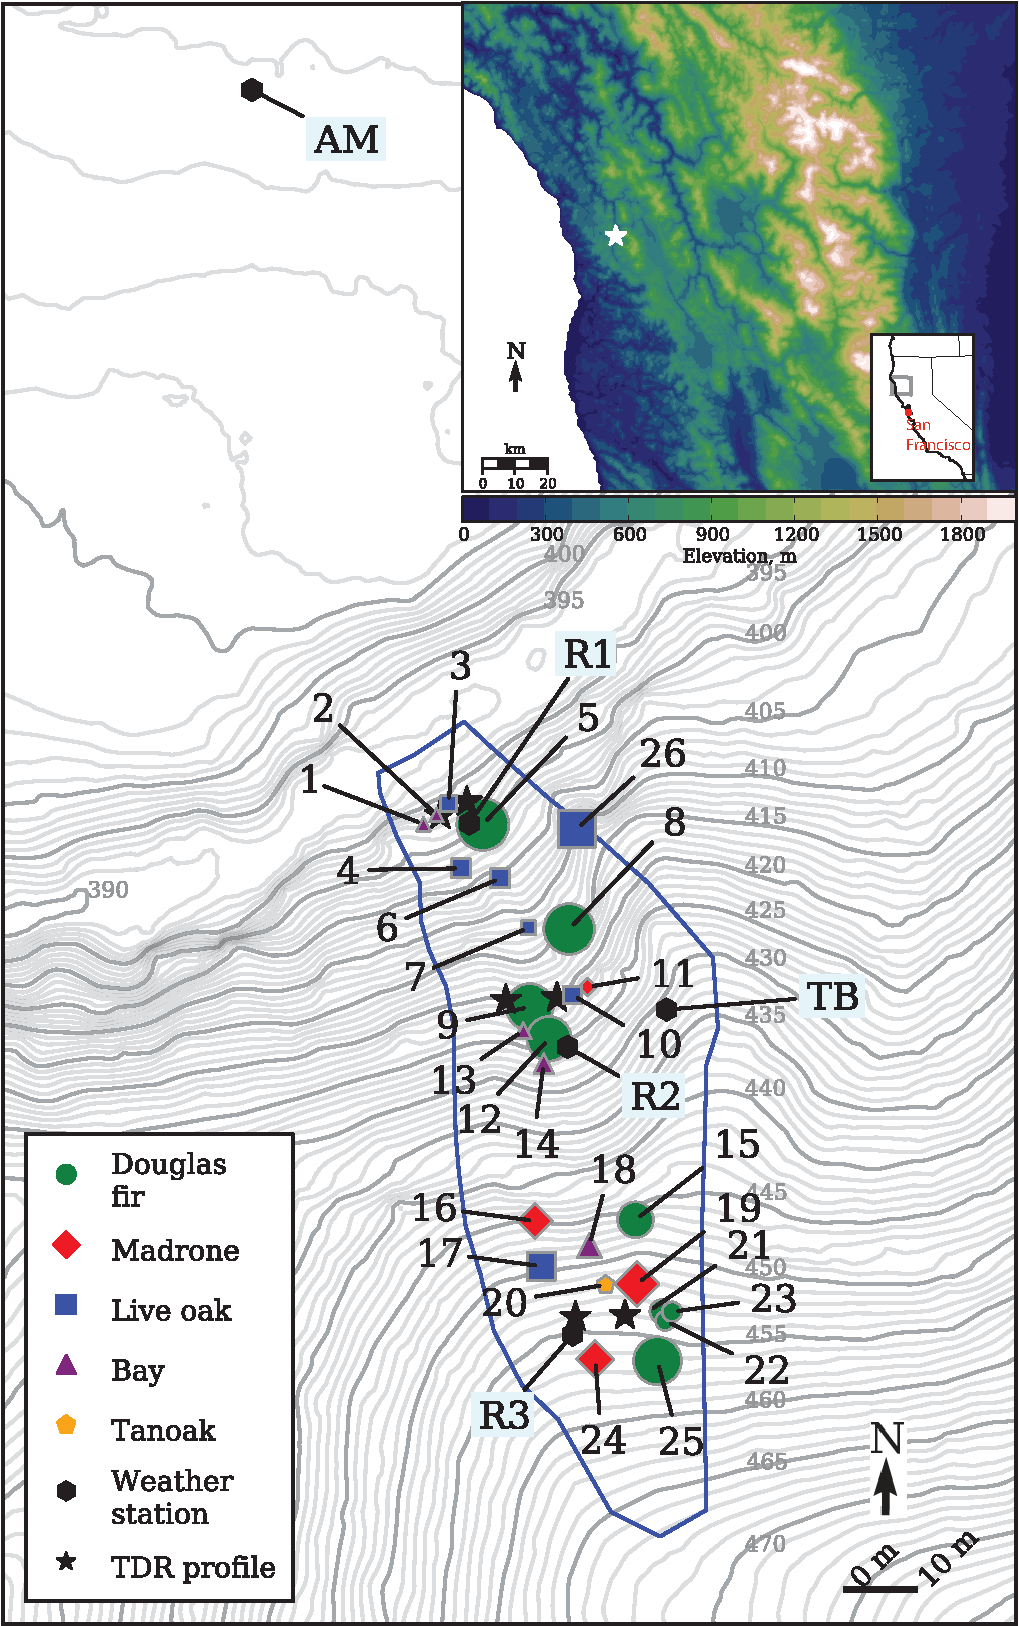
\includegraphics[width=0.7\textwidth]{ch1-sapflow/figures/Figure01.pdf}
\caption{Site map, showing topography, weather stations (R1, R2, R3, TB, AM), TDR profiles, and trees instrumented with sap flow sensors.  Symbols for instrumented trees are scaled by the tree diameter.  Tree numbers correspond with those in Table \ref{tbl:tree_props}.  Light gray numbers show elevation above sea level, in m.  Large inset: regional topography near the Angelo Coast Range Reserve (white star) [\cite{globe}].  Small inset: California, with gray box outlining the region displayed in the large inset, and red dot showing San Francisco.}
\label{fig:sapflow_map}
\end{figure}

The study site (39.729$^{\circ}$N, 123.644$^{\circ}$W) is located in the University of California Angelo Coast Range Reserve (ACRR) in Mendocino County, northern California, about 260 km north of San Francisco (Figure \ref{fig:sapflow_map} inset).  The ACRR sits in the Eel River watershed about 16 km east of the Pacific coast, just outside the coastal fog belt in the complex topography of the California Coast Range. The highest point in the ACRR, Cahto Peak, has an elevation of 1300 m above sea level, and the base elevation of the reserve is 400 m above sea level.
	
The field site, known as ``Rivendell'', is a small (4000 m$^2$), north-facing hillslope that drains to Elder Creek, a tributary of the South Fork Eel River (Figure \ref{fig:sapflow_map}).  Rivendell is the subject of an interdisciplinary collaborative project to study the lifecycle of water through a steep hillslope, and over 700 separate instruments have collected over 100 million data points between 2007 and May 2012.  The site has an average slope of approximately 32 degrees.  The subsurface structure consists of a thin soil mantle over a layer of highly fractured sedimentary rock, underlain by unweathered bedrock with very low permeability.  The fractured, weathered bedrock zone transitions with depth from relatively soil-like granular material to low-permeability bedrock bounded by fractures.  Both the soil mantle and the weathered rock layer are thicker at the hill crest (60 cm soil and 20 m weathered rock) and thinner at the base of the hill (0-30 cm soil and 5 m weathered rock) [\cite{rempe2010}].

The old-growth forest in the ACRR consists primarily of Douglas-fir (\textit{Pseudotsuga menziesii}), coast redwood (\textit{Sequoia sempervirens}), interior live oak (\textit{Quercus wislizeni}), tanoak (\textit{Notholithocarpus densiflorus}), Pacific madrone (\textit{Arbutus menziesii}), and California bay (\textit{Umbellularia californica}).  In the Eel River watershed, Douglas-fir constitutes approximately 40\% of tree basal area [\cite{woudenberg2010forest}] and is commonly associated with Pacific madrone, tanoak, live oak, and other species in the Pacific Douglas-fir alliance in coastal northern California [\cite{usda}].  At the study site, Douglas-firs form the overstorey, with heights up to 55-60 m, while live oaks, bays, Pacific madrones, and tanoaks form the lower canopy, reaching heights of approximately 20 m.  Below the lower canopy, there are smaller (5-10 m) trees of all species. There is no dense ground cover. Douglas-firs, live oaks, tanoaks, and bays are evenly distributed across the hillslope, while Pacific madrones occur more frequently upslope.  Douglas-fir is a needleleaf tree, while live oaks, tanoaks, Pacific madrones, and bays are broadleaf trees, but all of these species are evergreen. The rooting depths of trees at this site have not been determined, but during drilling of wells at the site, roots of unidentified species were observed most densely in the top several meters and with decreasing density to a depth of 15.2 m.

Climatic variables, including air temperature (\textit{T}, $^{\circ}$C), relative humidity (\textit{RH}, \%), solar radiation (\textit{I}, W/m$^2$), and precipitation (\textit{P}, mm), are measured at five weather stations at the site (Figure \ref{fig:sapflow_map}).  One weather station (TB) is located approximately 30 m above ground in the tree canopy, three weather stations (R1, R2, and R3) are located 1 m above the ground in an along-slope transect, and one weather station (AM) is located in an open meadow with full clearance, across the stream from the site.  The weather stations on the site (TB, R1, R2, and R3) are used here to characterize the \textit{VPD} at the site (\textit{T} and \textit{RH} from Vaisala HMP45C-L sensors at R1, R2, R3, and from a Vaisala WXT510 sensor at TB; Vaisala, Helsinki, Finland), while the meadow weather station (AM) is used for unobstructed \textit{I} and gross \textit{P} (Li-Cor LI200X-L pyranometer, Li-Cor, Lincoln, NE, USA; and Campbell Scientific TE525 tipping bucket rain gauge, Campbell Scientific, Logan, UT, USA).  All meteorological and soil moisture measurements were recorded with CR1000 dataloggers (Campbell Scientific) at intervals of 15 minutes until 2010 and 5 minutes beginning in 2010, and transmitted wirelessly and automatically to an online server; the entire system is powered only by solar cells.

Both shallow soil moisture and groundwater level are measured at Rivendell.  Depth profiles of $\theta$ (with a sensor placed every 5 to 10 cm down to a depth of 50 to 70 cm) are measured continuously with time domain reflectometer sensors (TDR; TDR100, Campbell Scientific) at six locations on the hillslope (Figure \ref{fig:sapflow_map}).  The TDR sensors are 7.5 cm long and are located in \textit{in situ} material: small trenches were dug in order to insert the probes horizontally into the soil or soil-like material in rock fractures, after which the trenches were backfilled with excavated material.  Measured dielectric values are converted to volumetric $\theta$ (m$^3$ water/m$^3$ total) using the standard Topp equation [\cite{topp1980electromagnetic}].  Groundwater level is monitored at 12 on-site wells.

Volumetric $\theta$ measurements are filtered to exclude values outside the sensor's valid range and averaged over each day to reduce noise (no diurnal cycle is evident at this site, in contrast to other Douglas-fir sites [\cite{brooks2006}; \cite{Warren:2007ly}]).  The daily-average values are then averaged across all depths for each profile; each profile average is normalized by its maximum to convert to relative $\theta$ (\%); and the six profiles on the slope are then averaged to produce a site-averaged $\theta$ time series.  The conversion to relative soil moisture is performed because no site-specific TDR calibration was performed.  We explain our reasoning for the site averaging in the Discussion, Section \ref{sec:sapflow_soilmoisture}.

\subsection{Sap flow measurement}
Sap velocity, the velocity of water through the xylem parallel to the axis of the tree trunk, is measured in 26 trees using 39 heat ratio method sensors (ICT International, Armidale, Australia; \cite{burgess2001improved}) installed 1 m above the ground in the tree trunks.  The tree locations, species, and diameters at breast height are shown in Figure \ref{fig:sapflow_map}, with the symbol size scaled by tree diameter, and the properties of each sensor are listed in Table \ref{tbl:tree_props}.  The trees were chosen to represent the distribution of tree species and sizes on the hillslope, within the constraints of accessibility on the steep slope and a limited number of sensors.  Multiple trees were instrumented for each species except tanoak (1 tree), which was sparse on this hillslope (uncharacteristically for this region.)  Before installing the sensors, bark was removed to the cambium from an approximately 5 cm x 5 cm area.  Each sensor measures the velocity of a heat pulse emitted by the sensor at two radial depths in the xylem: 12.5 mm and 27.5 mm.  These depths are not precise because of minor errors in sensor placement; errors in probe spacing are corrected using the procedure in \cite{burgess2001improved}.  For this procedure, we assume zero flow at times when water stress is expected to be minimal: pre-dawn (within 3 hours before sunrise), high relative humidity (between 92 and 95\%), no solar radiation, no daily rain, and between January and March.  Sensors were moved in late 2010 to minimize wounding, creating two stages of deployment (2009-2010, and 2011.)  Because we did not measure wound diameters around the probes (as that would be destructive), we assume a wound diameter of 0.2 mm (a central value from Table 1 in \cite{burgess2001improved}) for all sensors; the wound correction is a linear factor and is thus removed by the normalization described below (Section \ref{sec:normalization}).  Heat pulse velocity was recorded on ICT SL5 Smart Loggers (ICT International, Armidale, Australia) at 30-minute intervals.

\begin{table}
  \caption{Sap flow sensor properties, including tree, sensor ID, stage of deployment, species, DBH (diameter at breast height), nearest weather station, active depth (radial sensor position with larger sap velocity), 99.5th percentile instantaneous sap velocity for each sensor position, 12.5 mm - 27.5 mm sensor correlation ($R^2$ coefficient comparing velocities at the two measured radial positions), 99.5th percentile daily integral sap velocity for the active sensor depth, lag time of sap velocity relative to radiation, lag time of sap velocity relative to $VPD$, wood dry density at the two sensor positions, and wood water content at the two sensor positions.}
  \label{tbl:tree_props}
  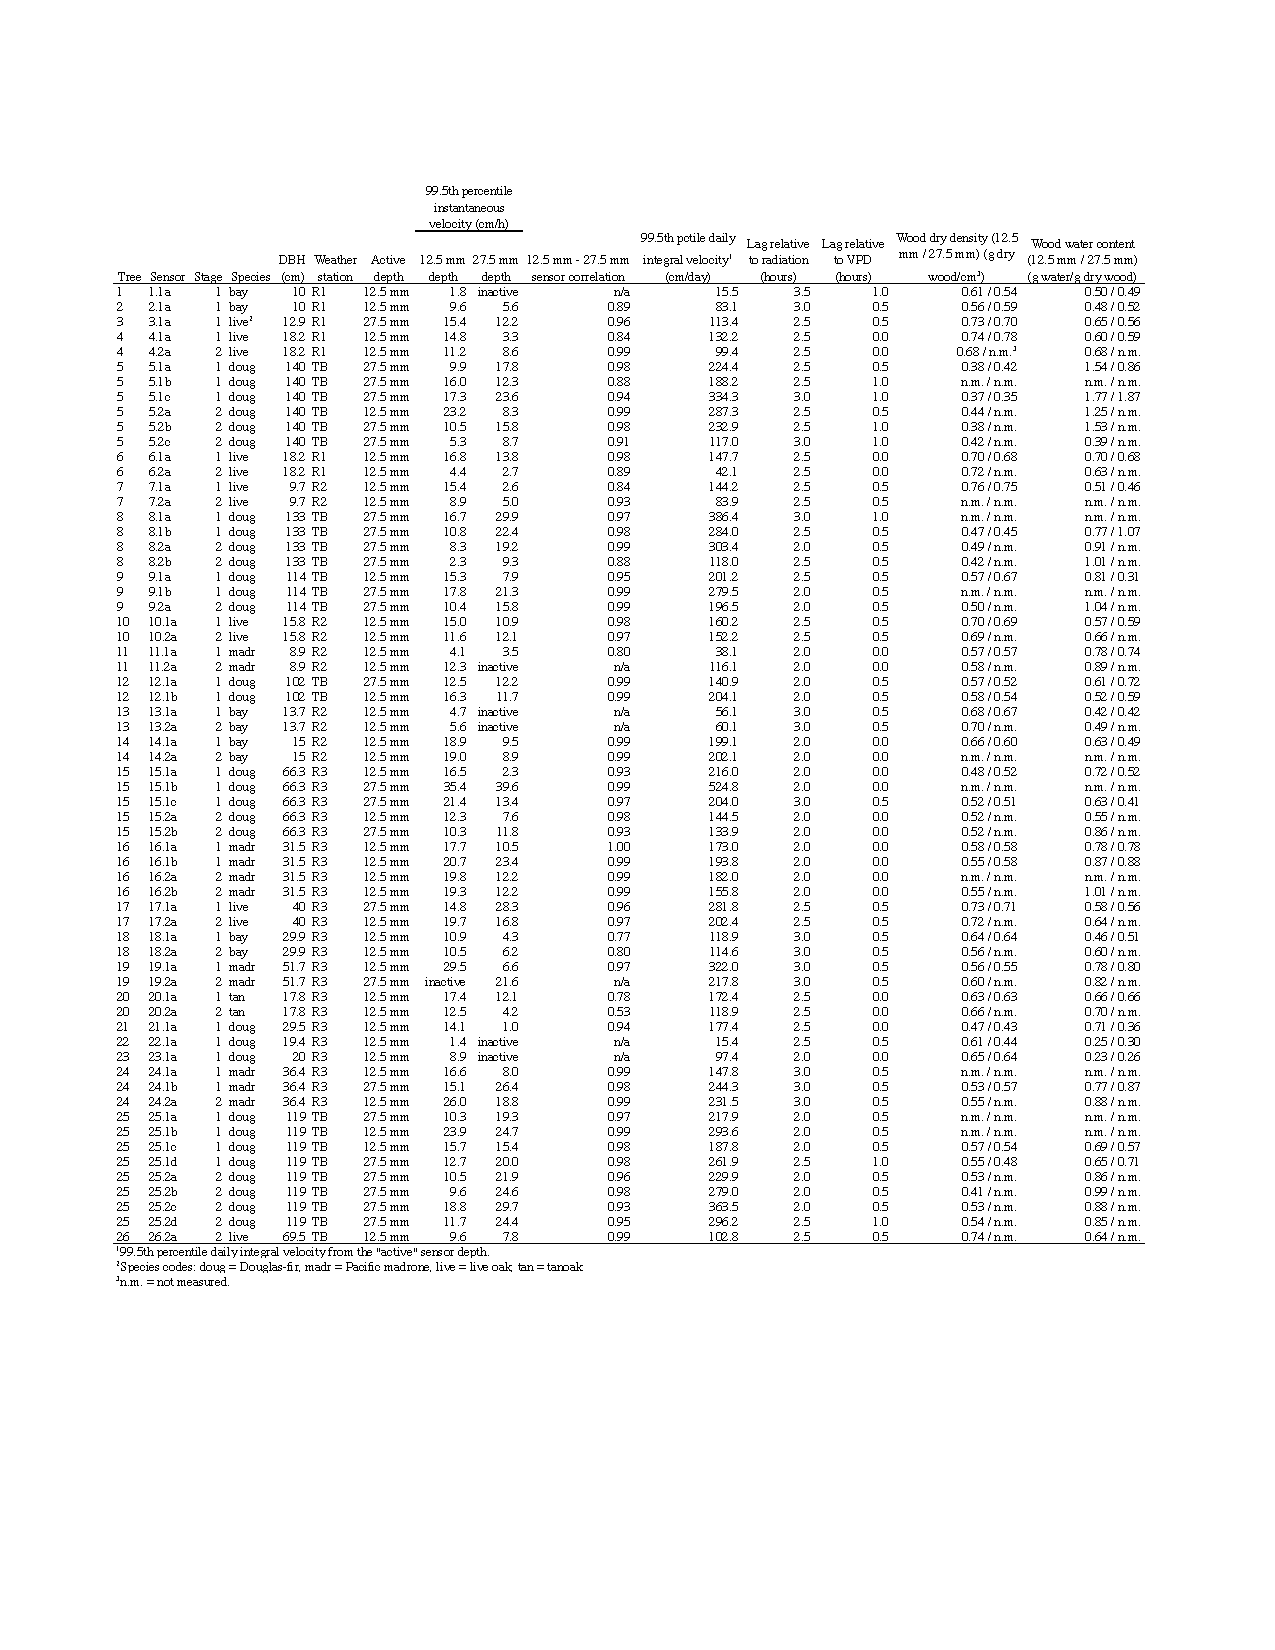
\includegraphics[width=\linewidth]{ch1-sapflow/tables/Table1_cropped.pdf}
\end{table}

Wood density and water content were measured by taking cores with an increment borer in October 2010 and October 2012, and these properties are used to convert heat pulse velocity to sap velocity [\cite{burgess2001improved}].  For several sensors, wood density and water content were not measured (Table \ref{tbl:tree_props}); for these sensors, the species-averaged values were used.  Because water content was only measured once at the end of each stage, we used a constant value throughout the year.  Uncertainties associated with this assumption are discussed in Section \ref{sec:sapflow_soilmoisture}.

For the following analyses, for each sensor, the depth with the larger magnitude of velocity (i.e. the most ``active'' depth) is chosen.  Sap velocity is known to vary radially through the sapwood [\cite{cohen1985determination}; \cite{vcermak1992radial}; \cite{nadezhdina2002radial}; \cite{ford2004assessing}]; in our measurements, the velocities at 12.5 mm and 27.5 mm differed in magnitude but were highly correlated for almost all sensors ($R^2$ values listed in Table \ref{tbl:tree_props}); as such, we include only one depth per sensor in order to avoid redundancy.

Finally, we add the caveat that we treat sap velocity as proportional to transpiration.  We discuss this assumption in Section \ref{sec:sapflow_soilmoisture}.

\subsection{Normalization}
\label{sec:normalization}
For most of our analyses, we use normalized sap velocities.  Normalizing allows us to compare temporal dynamics and environmental responses between sensors with very different absolute magnitudes, and eliminates the time-invariant differences in absolute velocity due to azimuthal, radial, or between-tree variation in wood properties.  We employ normalization on two time scales.   The first normalizes instantaneous (30-minute frequency) measurements by dividing by the 99.5th percentile value of that sensor (to avoid normalizing by an outlier); this normalization is used for analyzing responses to environmental drivers (Sections \ref{sec:mcmc} and \ref{sec:envresponse}).  In the second, daily integrals of sap velocity are normalized by dividing by the 99.5th percentile daily integral for each sensor; the normalized daily integrals are used for analyzing seasonal dynamics (Sections \ref{sec:pca} and \ref{sec:seasonal}), since the diurnal cycle is removed.  Sensors are normalized separately for each stage of deployment, because azimuthal variations in wood properties caused differences in absolute magnitude of velocity when sensors were moved within a tree.

\subsection{Principal Component Analysis}
\label{sec:pca}
We use principal component analysis (PCA) to find the dominant spatial and, importantly, temporal sap flow patterns in the sap flow dataset, and to compare the dominant seasonality patterns between trees, across space and between species.  PCA, also known as empirical orthogonal function analysis [\cite{lorenz1956empirical}], reduces a dataset with many points in space and time to a few orthogonal patterns that explain most of the variance. These orthogonal patterns are determined empirically from the data, as the eigenvectors of the covariance matrix.  PCA yields a series of temporal functions (PCs), with a corresponding series station weighting factors (EOFs), which represent how strongly each time function (PC) contributes to the actual time series at a given station.  The pairs of time-space functions (PC$_m$ and EOF$_m$) are ordered by the fraction of the total dataset variance that each explains.

We perform PCA separately on each of the two stages of sensor deployment (2009-2010, and 2011), because many of the time series were discontinuous across the sensor move; many sensors failed after the move or were placed in roots, which were not analyzed in the present study.  In order to maximize the amount of data included in the analysis, we performed PCA on the two stages separately.  Performing PCA on the two stages also has the advantage of providing replication of the dominant patterns of variability; similarity between results from the two stages would indicate interannual robustness of the seasonal patterns.

Days with missing data are excluded.  The analyses are performed on normalized daily integral values, subtracting each sensor's mean for the analysis period to focus on the temporal variability. The analysis is performed in Python, using the NumPy linalg function \textit{eig}. In the following, we focus on the first two PC-EOF pairs for each analysis, as they together explain over 90\% of the variance.

\subsection{MCMC estimation of environmental response parameters}
\label{sec:mcmc}
We quantify the relationship between each sensor's instantaneous sap flow and environmental drivers using the Jarvis model [\cite{jarvis1976interpretation}], which parameterizes stomatal conductance in terms of empirical functions of \textit{VPD}, \textit{I}, and $\theta$.

We begin with the assumption that each sensor's instantaneous normalized sap velocity ($v_n$, unitless) is proportional to the tree's transpiration ($E$, liters/day), scaled by a multiplier, $\alpha$ (liters/day), the product of maximum sap velocity, sap wood cross-sectional area, and the profile of sap velocity as a function of radius:

\begin{equation} % equation 1
\label{eqn:sf1}
E = \alpha \cdot v_n.
\end{equation}

Transpiration also equals the product of the tree's bulk canopy conductance ($g_c$, liters/day/kPa) and the leaf-to-air vapor pressure difference (which we approximate with the air \textit{VPD}.)  Thus,

\begin{equation} % equation 2
E = g_c \cdot VPD.
\end{equation}

Following the Jarvis model, canopy conductance ($g_c$) is modeled as a maximum conductance ($g_{cmax}$, liters/day/kPa), reduced by empirical multiplicative functions, ranging from 0 to 1, of important environmental modifiers: \textit{VPD}, $\theta$, and $I$ [\cite{jarvis1976interpretation}; \cite{oren1999survey}; \cite{waring2011generalizing}].

\begin{equation}  % equation 3
\label{eqn:sapflow_jarvis_simple}
g_c = g_{cmax} \cdot f_{VPD}(VPD) \cdot f_{\theta}(\theta) \cdot f_I(I).
\end{equation}

The functions of environmental modifiers are analytical parameterizations based on previous empirical observations.  For the atmospheric evaporative demand function, $f(VPD)$, we use an asymptotic function [\cite{lohammar1980fast}; \cite{lindroth1986numerical}; \cite{dang1997regulation}],

\begin{equation}  % equation 4
\label{eqn:sapflow_fVPD}
f_{VPD}(VPD) = \frac{1}{1+VPD/D_o},
\end{equation}
where $D_o$ (kPa) describes the sensitivity of $g_c$ to \textit{VPD}.

The water supply function, $f(\theta)$, is modeled as a sigmoid function, chosen because it is a continuous function that represents the threshold limitation of transpiration by $\theta$ in very dry soils; this is a continuous functional form that approximates the piecewise-linear Feddes model [\cite{feddes}; \cite{chen2008observations}]:

\begin{equation}  % equation 5
\label{eqn:sapflow_soilmois}
f_{\theta}(\theta) = \frac{1}{1+\exp(-\beta(\theta-\theta_o))},
\end{equation}
where $\beta$ (unitless) measures the rate of decrease of transpiration at low $\theta$, and $\theta_o$ (unitless) is the value of $\theta$ at which the transpiration decline is centered.  These parameters can be related to the more standard stress point and wilting point of the Feddes model by estimating the $\theta$ at which the sigmoid function begins to decline (the stress point) and the $\theta$ at which the sigmoid function is approximately zero (the wilting point.)

The radiation function, $f(I)$, is modeled as a linear function, after \cite{waring2011generalizing}:

\begin{equation}  % equation 6
f_I(I) = \gamma \cdot (I-1000 \, {\rm W/m^2})+1,
\end{equation}
where $\gamma$ ((W/m$^2$)$^{-1}$) is the sensitivity of transpiration to \textit{I}, and $f(I)$ is prescribed to be maximum (equal to 1) at maximum \textit{I} (1000 W/m$^2$).

Thus, we model normalized sap velocity as a function of \textit{VPD}, $\theta$, \textit{I}, and five parameters (considering $g_{cmax}/\alpha$ (kPa$^{-1}$) as a single parameter):

% equation 7
\begin{align}
\label{eqn:sapflow_jarvis}
v_n & =  \frac{g_{cmax}}{\alpha} \cdot VPD \cdot f_{VPD}(VPD) \cdot f_{\theta}(\theta) \cdot f_I(I) \nonumber \\ 
& =  \frac{g_{cmax}}{\alpha} \cdot \frac{VPD}{1+\frac{VPD}{D_o}} \cdot \frac{1}{1+\exp(-\beta(\theta-\theta_o))} \cdot (\gamma \cdot (I-1000)+1).
\end{align}

We estimate these five parameters for each sensor using a Markov chain Monte Carlo (MCMC) method, described in the appendix (Section \ref{sec:sapflow_appendix}).  The MCMC method allows us to quantify uncertainty in the parameters and avoid local minima traps on the complex $\chi ^2$ surface that might hinder optimization algorithms.  Each sap flow sensor is matched with the nearest weather station: the canopy weather station (TB) is used for the overstorey trees, while the nearest ground station (R1, R2, or R3) is used for the understorey canopy trees, including small Douglas-firs.  Incoming \textit{I} measured in the open meadow (station AM, Figure \ref{fig:sapflow_map}) is used for all sensors, because \textit{I} was only measured at station AM.  \textit{VPD}, \textit{I}, and $\theta$ were subsampled to the 30-minute frequency of sap flow measurements.  For each tree, sap velocity is lagged relative to \textit{I} and \textit{VPD} by a lag time determined by the maximum lag correlation for that tree's average timeseries, similar to the procedure in \cite{dragoni2009decoupling}; lag times are listed in Table \ref{tbl:tree_props}.  The analysis is performed using times when \textit{I} was greater than zero (i.e., daytime observations) and \textit{VPD} was greater than 0.1 kPa.  Days with more than 2 mm of rain were excluded, because on those days leaves were probably covered with water and sap velocity thus was probably not controlled by stomatal response to the environment.  The site-averaged, daily-averaged $\theta$ is used for all sensors, as described in Section \ref{sec:sapflow_sitedesc}.  Parameters are also estimated for each species as a whole, using the average $v_n$ at each measurement from all sensors from a given species; these are referred to as the ``species-averaged timeseries" parameters.

\subsection{Estimates of regional transpiration}
\label{sec:sapflow_regmeth}
We use the species-averaged timeseries of normalized sap velocity, along with Forest Inventory and Analysis (FIA) [\cite{woudenberg2010forest}] observations of tree size and species distributions in the Eel River watershed, to estimate the contribution of each species to regional transpiration.  We estimate regional transpiration, rather than hillslope transpiration at our particular site, because regional distributions of trees by species and diameter are available from the FIA inventory, but no species-diameter inventory has been conducted at our particular site.  This scale jump requires simplifications and assumptions (described below), and as such, our calculations are a rough best estimate and an attempt to bound the range of possible forest transpiration in this region from a bottom-up perspective.  

Transpiration was estimated using Equation \ref{eqn:sf1}, with $v_n$ calculated using the species-averaged timeseries Jarvis parameters, and $\alpha$ disaggregated as follows.  Transpiration for a single tree ($E_{tree}$, cm m$^2$/hr) is

% equation 8
\begin{align}
E_{tree} & = \int_{r_{inner}}^{r_{outer}} 2\pi r \, v(r) \, \mathrm{d}r \nonumber \\ 
& =  \int_{r_{inner}}^{r_{outer}}  2\pi r \, v_{max} \, v_{n} \, f_{prof}(r) \, \mathrm{d}r,
\end{align}
where $r$ is radial position on a cross-section of the tree, $r_{inner}$ is the radial position of the sapwood-heartwood boundary (meters), $r_{outer}$ is the radial position of the sapwood-bark boundary (meters, here treated as approximately equal to half the tree diameter at breast height, $d/2$), $v(r)$ is the sap velocity as a function of radial position in the sapwood (cm/hr), and $f_{prof}(r)$ is a linear function between 0 and 1 describing the radial profile of sap velocity relative to the velocity at the outer edge (described below).  In this equation, $v_n$ and $v_{max}$ can be pulled out of the integral, and the resulting term $2\pi \, v_{max} \, \int_{r_{inner}}^{r_{outer}}  r \, f_{prof}(r) \, \mathrm{d}r$ is equal to $\alpha$ in Equation \ref{eqn:sf1}.

The thickness of the sapwood is estimated using two site-specific sapwood thickness--diameter relations, derived from 21 tree cores taken near Rivendell (15 Douglas-fir samples ($R^2=0.88$) and 6 Pacific madrone samples ($R^2=0.83$)):
\begin{align}
\label{eqn:sapwood}
w_{sap,Douglas-fir} = 0.12d+0.0089\\
w_{sap,madrone} = 0.1d+0.0071 ,
\end{align}
and
\begin{equation}
r_{inner} = d/2-w_{sap},
\end{equation}
where $w_{sap}$ is sapwood thickness (m).  Our Douglas-fir relationship is roughly similar to the one found by \cite{smith1966variation} for Douglas-fir.  

In addition, for other broadleaf species, we use the ring-porous equation from \cite{wullschleger2001transpiration}:
\begin{equation}
\label{eqn:sapwood2}
r_{inner,Wullschleger} = \sqrt{\left(\frac{d}{2}\right)^2-\frac{1.637d^{0.56}}{\pi}}.
\end{equation}
This equation is used for non-Pacific-madrone broadleaf species.

Sap velocity was approximated as a linear function of radial position in the sapwood, based on observations that sap velocity is often lower in the inner sapwood than in the outer sapwood [\cite{ford2004assessing}; \cite{cohen1985determination}; \cite{vcermak1992radial}; \cite{nadezhdina2002radial}].  The velocity at the outer edge of the sapwood was estimated as the product of a time-invariant maximum velocity ($v_{max}$, cm/hr) and a time-varying normalized velocity ($v_n$, unitless), approximated as the species-averaged timeseries of measured normalized sap velocity.  $v_{max}$ values for each species were treated as independent of tree diameter and were approximated with the species-averaged maximum instantaneous velocities from Table \ref{tbl:sapflow_maxvel}.  Sap velocity is assumed to be independent of azimuth, or equivalently, we assume that $v_{max,sp}$ is an average of the maximum velocity around the bole of a tree.

\begin{table}
  \caption{Species-averaged maximum sap velocities.}
  \label{tbl:sapflow_maxvel}
  \begin{tabular}{l r}
  \hline
  Species & Velocity (cm/h) \\
  \hline
  Douglas-fir & 18.2 \\
  Pacific madrone & 19.5 \\
  live oak & 14.0 \\
  bay & 10.1 \\
  tanoak & 15.0 \\
  \hline
  \end{tabular}
\end{table}

Because the radial profile of sap velocity is not well constrained with our measurements, we test three possible velocity profiles, with $v(r) = v_{max} \, v_n \, f_{prof}(r)$: (1) constant velocity across the sapwood ($f_{prof}(r) = 1$); (2) velocity decreasing linearly from $v_{max} \, v_n$ at the outer edge of the sapwood to $0.5 \, v_{max} \, v_n$ at the inner edge of the sapwood ($f_{prof}(r) = 1+\tfrac{0.5}{w_{sap}}(r-r_{outer})$ ); and (3) velocity decreasing linearly from $v_{max} \, v_n$ at the outer edge of the sapwood to 0 at the inner edge of the sapwood ($f_{prof}(r) = 1+\tfrac{1}{w_{sap}}(r-r_{outer})$ ).

Transpiration is scaled from a single tree to the regional scale using distributions of tree species and sizes measured in the Eel River watershed by the FIA program, binned by diameter in 5 cm bins [\cite{woudenberg2010forest}] (locations of FIA plots are intentionally ``fuzzed and swapped'' for privacy reasons, but the provided coordinates are ``similar'' to the true coordinates with an unspecified offset).  The FIA surveyed 321 forested plots within the Eel Watershed.  Figure \ref{fig:sapflow_abundances} shows $N_{i,sp}$, the number of trees per km$^2$ in each diameter bin ($i$) for major species categories in the watershed ($sp$), averaged over the 321 FIA plots.

\begin{figure}[here]
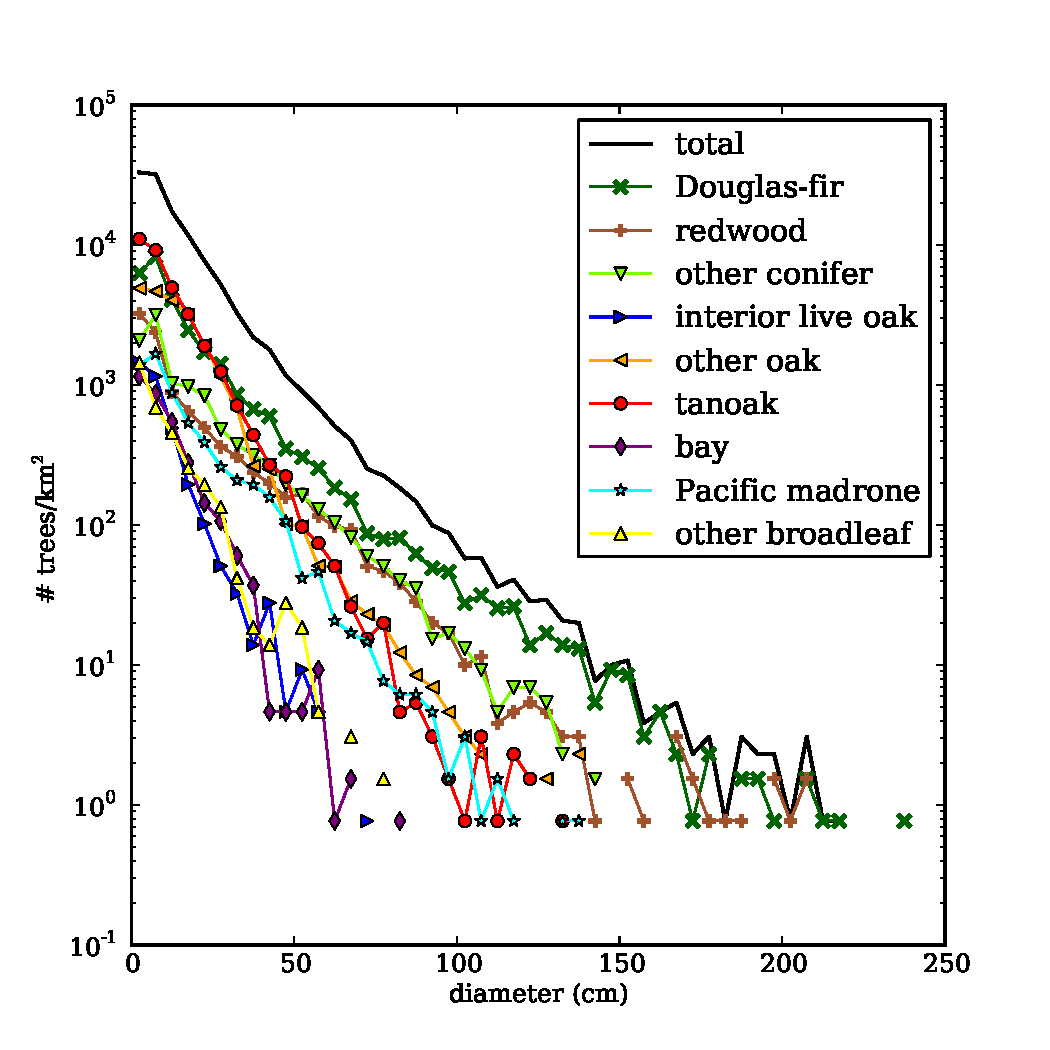
\includegraphics[width=0.9\textwidth]{ch1-sapflow/figures/Figure02.pdf}
\caption{Counts of trees per km$^2$ in major species categories, binned diameter; from FIA plots in the Eel River watershed [\cite{woudenberg2010forest}].  The category ``other conifer'' includes knobcone pine, Jeffrey pine, sugar pine, Western white pine, bishop pine, ponderosa pine, California foothill pine, white fir, grand fir, red fir, Pacific yew, western hemlock, incense cedar, and Sitka spruce.  The category ``other oak'' includes California live oak, canyon live oak, blue oak, Oregon white oak, California black oak, and California white oak.  The category ``other broadleaf'' includes bigleaf maple, California buckeye, red alder, white alder, giant chinkapin, and bitter cherry.}
\label{fig:sapflow_abundances}
\end{figure}

Regional transpiration due to each species (mm/d) is then estimated by summing individual tree transpiration of the species over all diameter bins ($i$):
\begin{align}
\label{eqn:transpreg}
T_{sp} &= \sum_{i} N_{i,sp} \, E_{tree,i,sp} \nonumber \\
&= 2\pi \, v_{max,sp} \, v_{n,sp} \, \sum_{i} N_{i,sp} \, \int_{r_{inner,i}}^{r_{outer,i}}  r \, f(r) \, \mathrm{d}r ,
\end{align}
and subsequently applying a unit conversion factor of $(10 \tfrac{mm}{cm}) (24 \tfrac{hr}{day}) (10^{-6} \tfrac{km^2}{m^2})$.  Total regional transpiration is estimated by summing transpiration estimated for all species, using the averaged time series of measured species to represent unmeasured but similar species.  All conifers, including redwoods, are assigned the Douglas-fir time series; all oaks, both evergreen and deciduous, are assigned the interior live oak time series; and all other unmeasured broadleaf trees are assigned the Pacific madrone time series, in order to give an upper-bound estimate on dry season transpiration.  Thus, we effectively bin species into categories of needleleaf evergreen and broadleaf evergreen; these assumptions are necessary because redwoods and major pine species were not measured due to their scarcity at our site.  In addition, we calculate regional transpiration in two extreme hypothetical cases, using the FIA total tree size distribution (black line in Figure \ref{fig:sapflow_abundances}): one case in which all trees are assigned the Douglas-fir time series, and another case in which all trees are assigned the Pacific madrone time series. 

The sap-flow-based regional transpiration estimates are compared with remotely-sensed MODIS-derived estimates of ET [\cite{mu2007development}].  The MODIS algorithm uses remotely-sensed LAI and modeled stomatal response based on an assigned plant functional type (which for this region is evergreen needleleaf forest), combined with meteorology from atmospheric reanalysis, to estimate stomatal conductance and ET.  No soil moisture or subsurface information is explicitly included.  Two spatial scales of the MODIS-derived estimate are presented: the 1 km x 1 km pixel nearest to Rivendell (pixel centered about 450 m east of Rivendell), and the average for all pixels in the Eel River watershed.  Our goals in comparing our estimated to the MODIS-derived estimate are a) to confirm that our estimates are the right order of magnitude, and b) to compare the seasonal timing of transpiration between the methods.



\section{Results}

\subsection{Environmental conditions}

\begin{figure}[here]
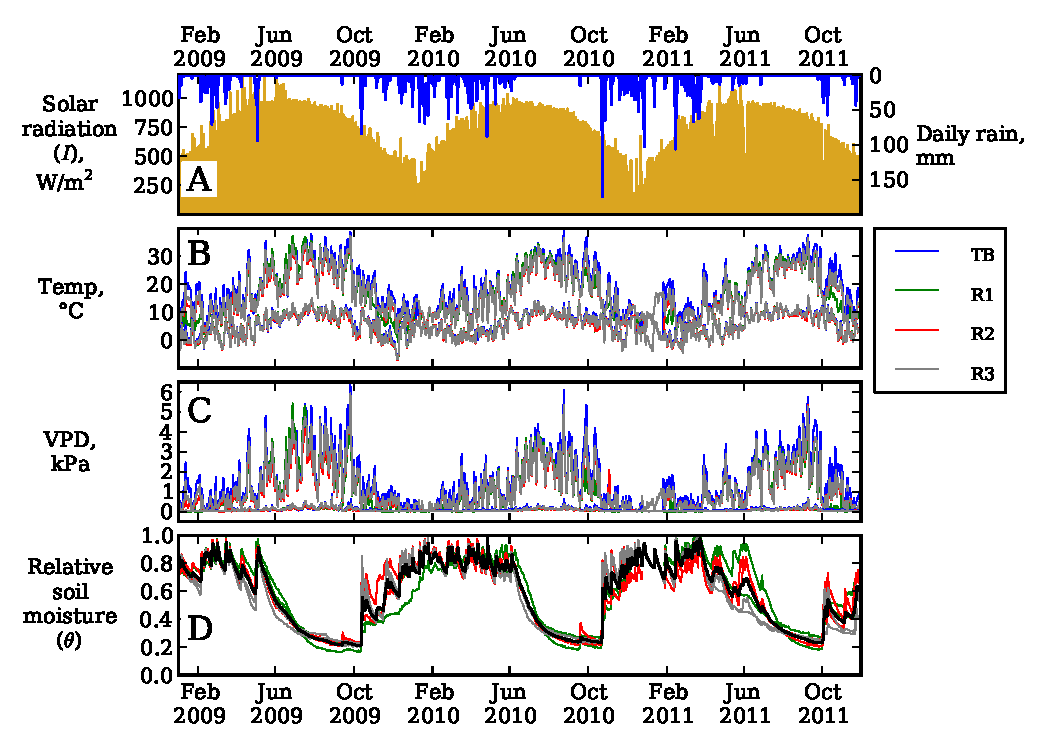
\includegraphics[width=0.9\textwidth]{ch1-sapflow/figures/Figure03.pdf}
\caption{Climatic and hydrologic time series: (a) solar radiation (\textit{I}, yellow) and daily rainfall (blue), both measured unobstructed in an open field; (b) daily minimum and maximum air temperature (\textit{T}) at ground stations (R1, R2, R3) and canopy station (TB); (c) daily minimum and maximum vapor pressure deficit (\textit{VPD}) at ground stations (R1, R2, R3) and canopy station (TB); (d) red, green, and gray: daily average relative soil moisture (\textit{$\theta$}), averaged over each of the 6 profiles shown in Figure \ref{fig:sapflow_map} (colors indicate the profile's nearest weather station, as in panel (b) legend); black: average of the 6 profile averages of relative soil moisture.}
\label{fig:sapflow_met}
\end{figure}

The ACRR has a Mediterranean climate with a marked winter wet season and summer dry season.  The wet season at the ACRR extends from approximately October through April (90\% of the annual precipitation fell in these months in 2009-2011), and very little rain falls during July through September (less than 1\% in 2009-2011; Figure \ref{fig:sapflow_met}(a)).  Clear sky \textit{I} is maximum in late June (summer solstice) and minimum in late December (winter solstice), and \textit{I} can be reduced by 50 to 90\% on cloudy days.  The annual cycle of \textit{T} lags behind that of \textit{I}, with a peak in July and August and a minimum in January or February. The mean July-September \textit{T} for 2009-2011 was 18$^{\circ}$C, and the mean December-February \textit{T} was 5$^{\circ}$C (weather station R3).  The annual cycle of \textit{VPD} follows that of \textit{T} and also peaks in July or August.  \textit{T} and \textit{RH} vary somewhat along the hillslope: on clear days, the air is warmer and drier in the upper canopy and upslope, and the air is cooler and more humid downslope (up to 10$^{\circ}$C cooler at downslope ground level than in the canopy at midday in winter; Figure \ref{fig:sapflow_met}(b) and (c)).  Mean annual \textit{P} in the vicinity of the ACRR (National Climatic Data Center GHCN precipitation station USC00048490, 18 km NNE of the ACRR; data from 1960-2000; XXXX \textit{Williams et al.} [2012]) is 1800 mm, with significant interannual variability (standard deviation of 500 mm); on average, 3\% ($\pm$3\% standard deviation) of annual precipitation falls in July through September.  During the study period, precipitation at Rivendell ranged between a minimum of 1500 mm in water year 2008-2009 and a maximum of 2100 mm in water year 2010-2011.

Water storage below ground is also highly seasonal. The water table, measured by 12 on-site wells, remains near 5 m below ground throughout the year at downslope wells, but upslope it ranges from $\sim$10 m below ground in the wet season to $\sim$20 m below ground in the dry season.   Soil moisture ($\theta$) is high and dynamic during the winter rainy season but dries to fairly steady and very low values during the summer dry season (Figure \ref{fig:sapflow_met}(d); \cite{salve2012rain}).  

\subsection{Sap velocities}

\begin{figure}[here]
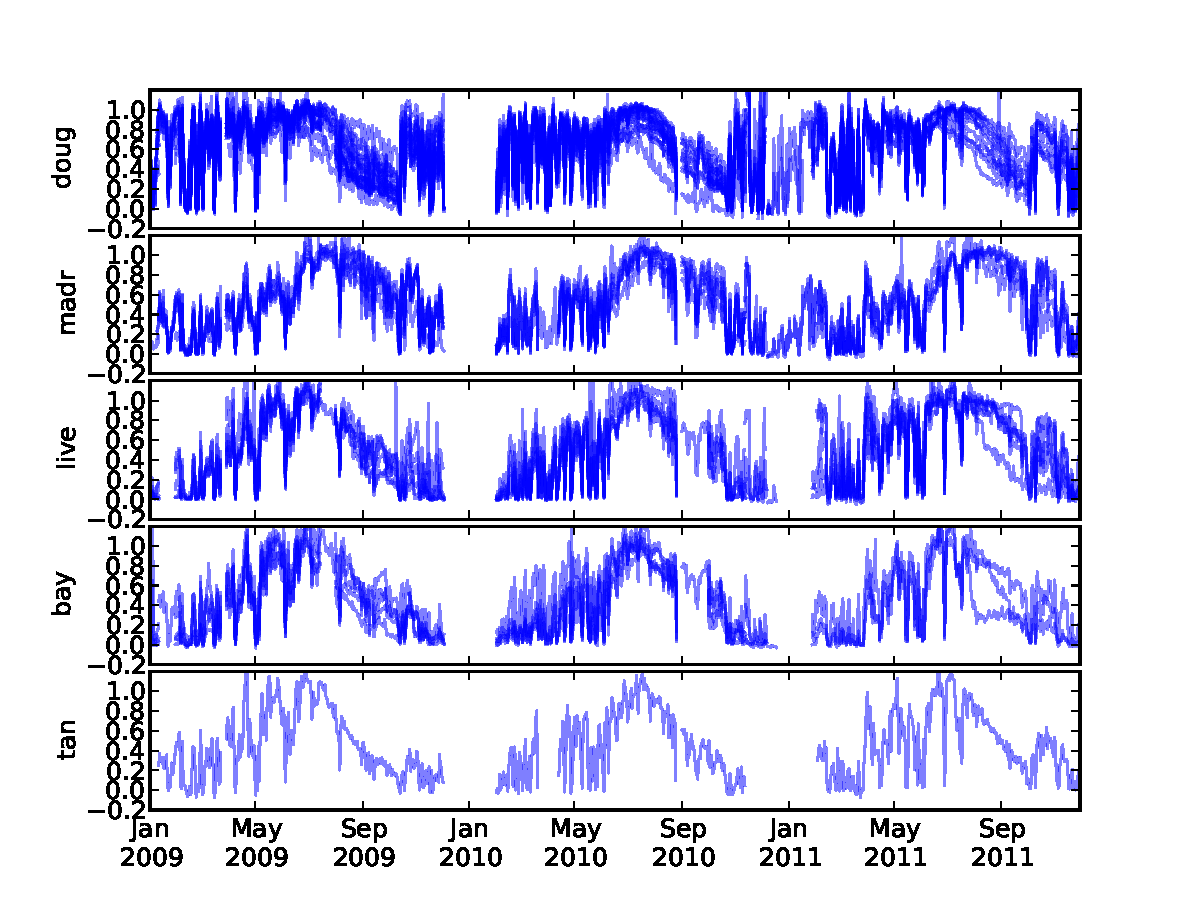
\includegraphics[width=0.9\textwidth]{ch1-sapflow/figures/Figure04.pdf}
\caption{Daily maximum normalized sap velocities for each sensor, separated by species.  Each sensor's line is slightly transparent, so that overlapping lines create darker blue colors.  Data gaps are due largely to power failure during times of low insolation.  Species codes: doug=Douglas-fir; madr=Pacific madrone; live=interior live oak; tan=tanoak.}
\label{fig:sapflow_normvel}
\end{figure}

The 99.5th percentile velocities for each sensor and each stage are listed in Table \ref{tbl:tree_props}, and the timeseries of daily maximum normalized instantaneous velocity for each sensor are shown in Figure \ref{fig:sapflow_normvel}, separated by species (only the daily maximum is shown for visibility.)  For the following analyses, we constructed tree-averaged timeseries for trees with multiple sensors by averaging the normalized velocities at each measurement time for all sensors in a given tree.  This tree-averaging was performed because sensors within a tree covaried strongly for all trees (Table \ref{tbl:sapflow_covar}), and thus sensors in the same tree were not independent.

\begin{table}
  \caption{Covariation of sap velocities within the same tree.}
  \label{tbl:sapflow_covar}
  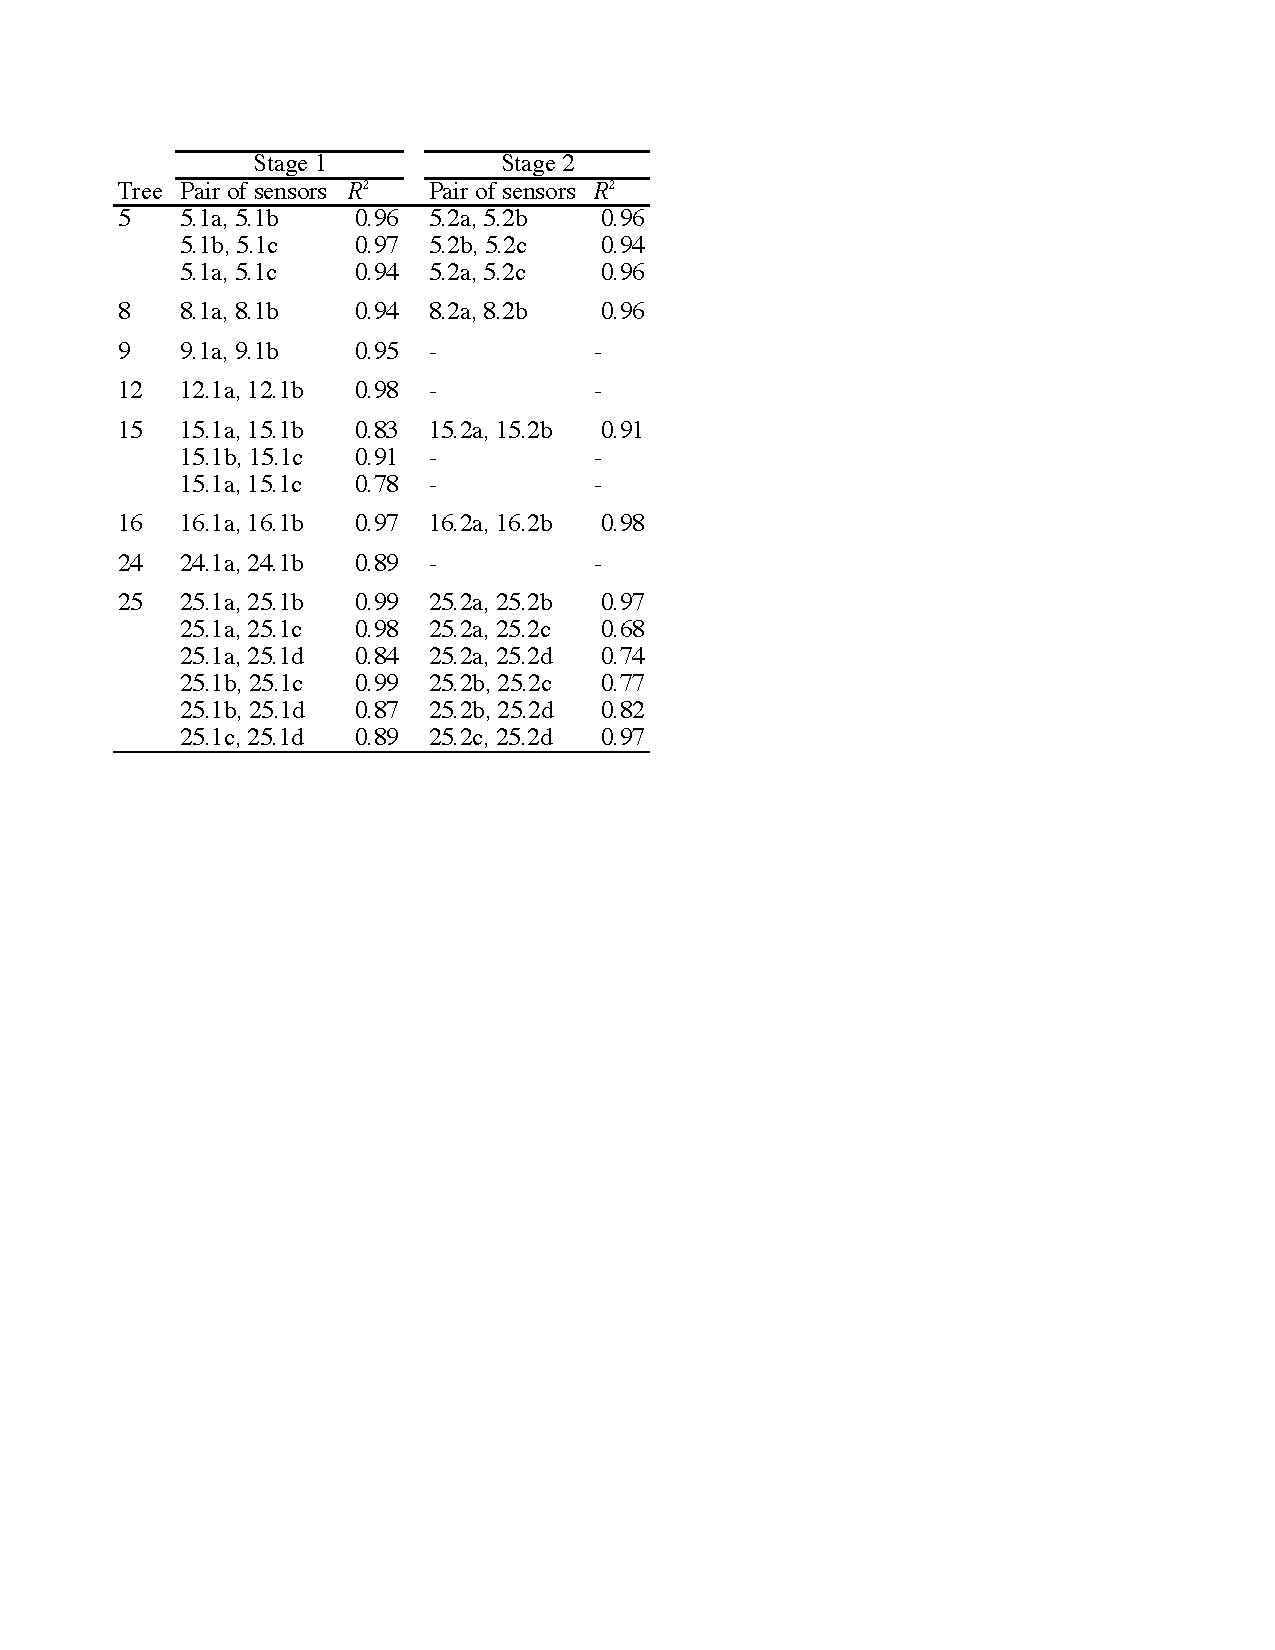
\includegraphics[width=\linewidth]{ch1-sapflow/tables/TableA1.pdf}
\end{table}

\subsection{Seasonal patterns: Principal Component Analysis}
\label{sec:seasonal}

\begin{figure}[here]
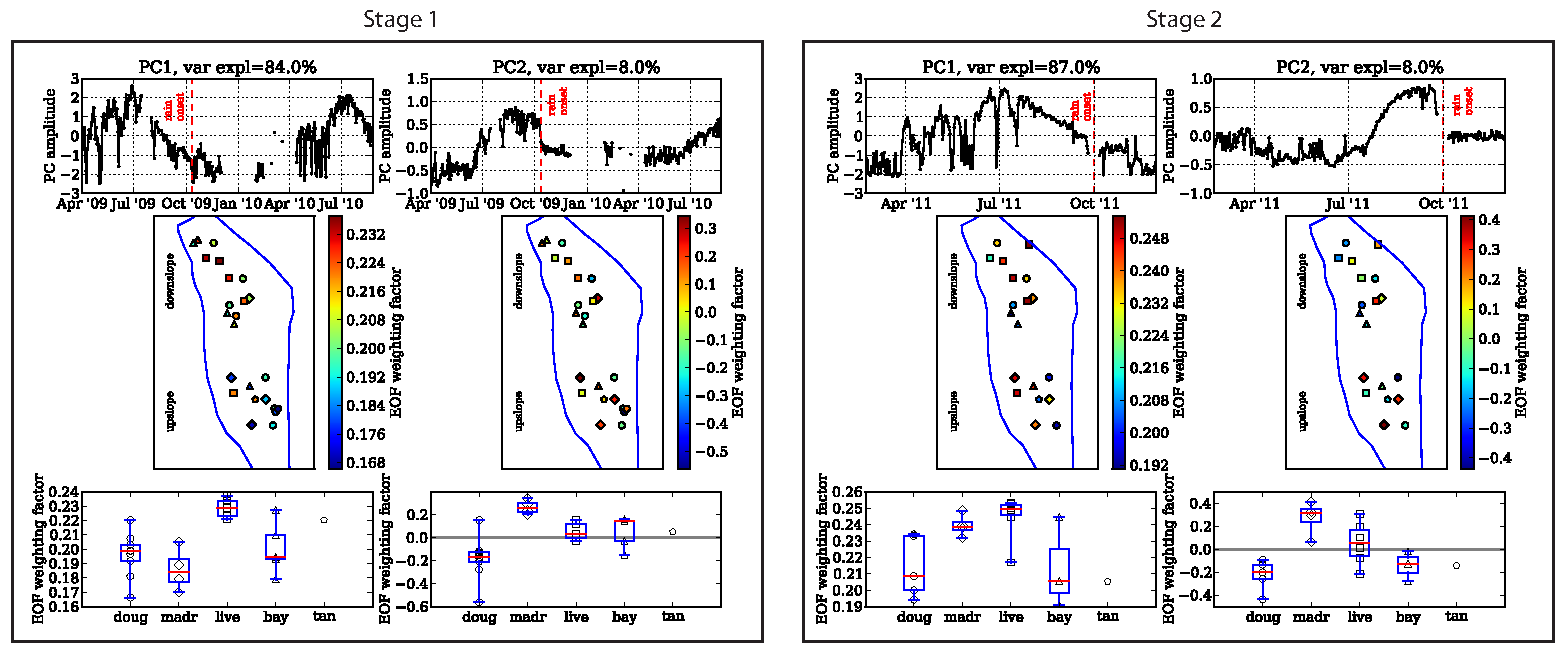
\includegraphics[width=0.9\textwidth]{ch1-sapflow/figures/Figure05.pdf}
\caption{PCA results for all sensors, for stage 1 (left box) and stage 2 (right box).  Within each stage, left column: PC/EOF 1, right column: PC/EOF 2.  Top row: principal component time patterns.  Circles show days included in the analysis.  Gaps represent periods of missing data longer than 4 days.  Middle row: maps of EOF weighting factors for all trees included in the analysis.  Symbol shape indicates species, as in Figure \ref{fig:sapflow_map}.  Bottom row: EOF weighting factors, sorted by species.  Box plot divides the quartiles of the distribution; red line shows the median.  Both the PCs and EOFs are unitless, because the analysis used normalized velocities.}
\label{fig:sapflow_eof}
\end{figure}

The time pattern that explains the most variance among all sap flow sensors, PC1, represents the common annual cycle, with a peak in early July and lower values through the winter, mirroring the annual cycle of solar radiation (Figure \ref{fig:sapflow_eof}, left column in each stage).  PC1 also contains the abrupt drops in sap flow on rainy days in winter and spring, when almost all sensors have very low sap velocity.  The annual cycle pattern is evident in PC1 for both stages, and PC1 explains 84\% of the variance in stage 1 (2009-2010) and 87\% of the variance in stage 2 (2011).  All sensors in both stages have positive weighting factors for PC1, meaning that all sensors display a component of this annual cycle pattern.  In stage 1, downslope trees tend to resemble PC1 more strongly than do upslope trees (i.e., have larger positive weighting factors).

The time pattern that explains the next-largest fraction of the variance, PC2, acts as a phase offset from the PC1 annual cycle, with a positive peak in the July-October dry season and negative values for the rest of the year (Figure \ref{fig:sapflow_eof}, right column in each stage).  Again, the PC2 pattern is similar between the two stages of deployment.  A positive EOF2 weighting factor for PC2 indicates greater July-October transpiration than PC1 and less November-June transpiration, and thus a shift in the peak season of transpiration later into the dry season.  On the other hand, a negative EOF2 weighting factor indicates less July-October transpiration compared to PC1 and greater transpiration in the rest of the year, and thus indicates a shift in peak transpiration earlier toward the wet spring.  PC2 explains 8\% of the variance in both stages.

The direction of the transpiration phase shift is species-specific.  Pacific madrones have the most positive weighting factors for PC2 in both stages, indicating a phase shift of peak transpiration later into the dry season (Figure \ref{fig:sapflow_eof}, bottom right panel in each stage).  Douglas-firs, in contrast, almost all have negative values, indicating a phase shift earlier toward the wet spring season.  Live oaks, bays, and the tanoak have weighting factors closer to zero, indicating less phase shift away from the PC1 pattern.

Additionally, the PC2 time pattern shows an abrupt decrease at the onset of the rainy season in October of each year.  Thus, Pacific madrone sap velocities, with positive PC2 amplitudes, decrease sharply at the onset of the rainy season, while Douglas-fir velocities, with negative PC2 amplitudes, increase sharply.

\subsection{Sensitivities to environmental drivers}
\label{sec:envresponse}

These PC/EOF patterns are empirical, indicating the dominant patterns of variability and demonstrating that there is a seasonal offset of transpiration between evergreen tree species at this site.  In order to investigate the drivers of this difference, we quantify the response of sap velocity to environmental variables.

\begin{figure}[here]
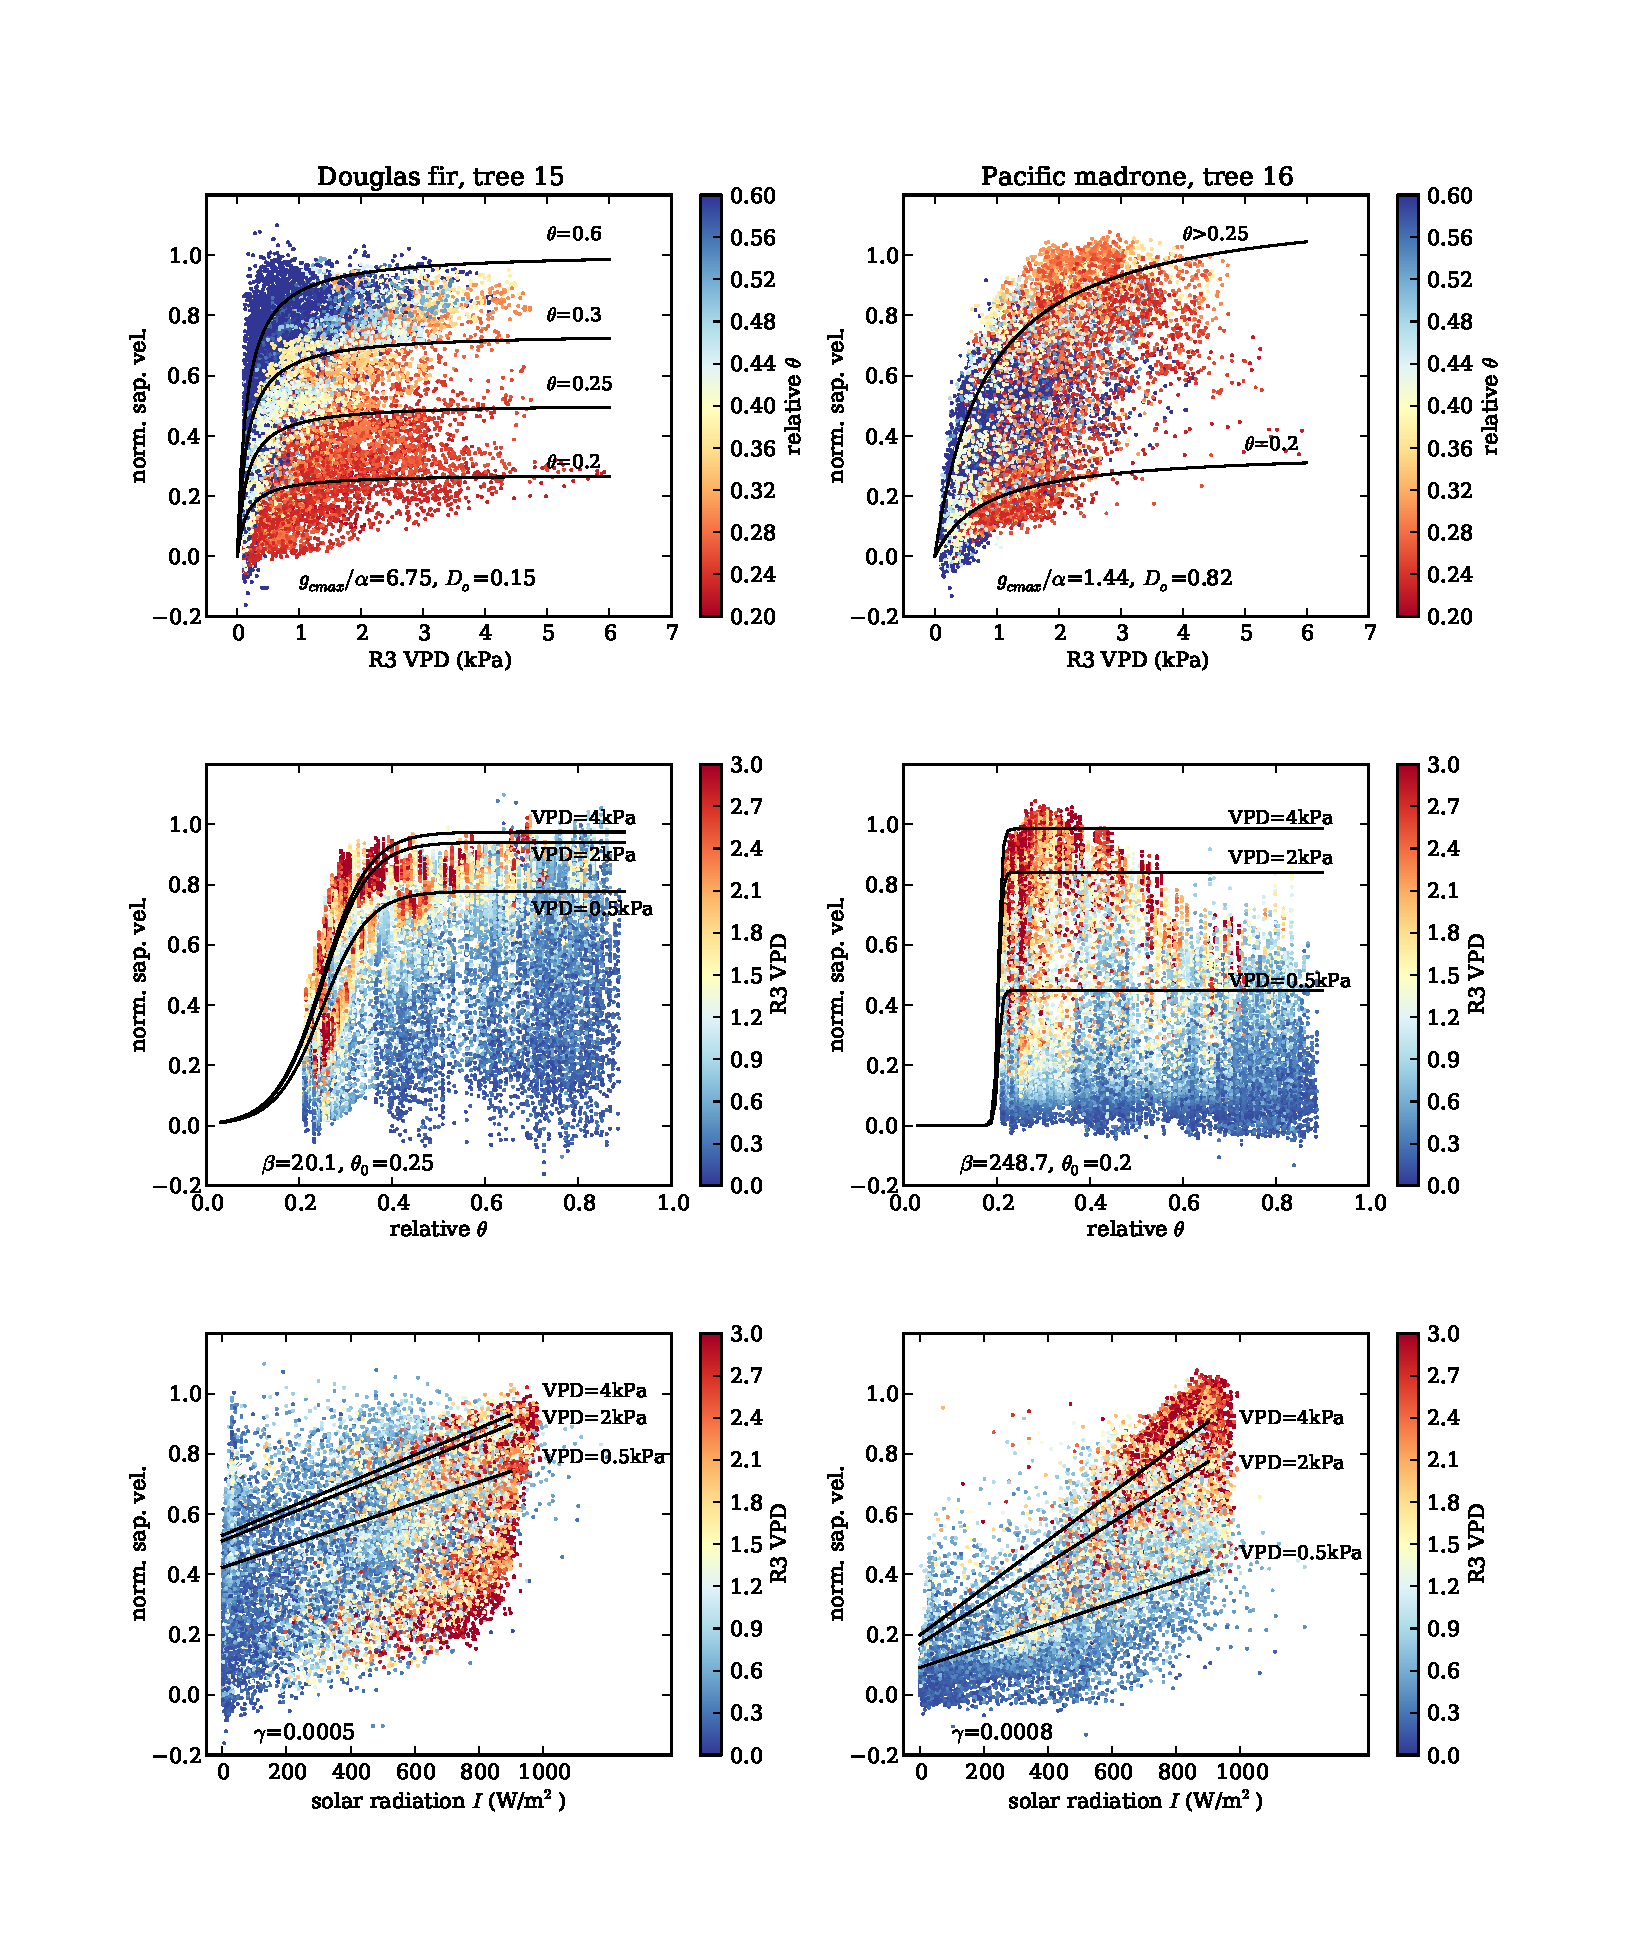
\includegraphics[width=0.9\textwidth]{ch1-sapflow/figures/Figure06.pdf}
\caption{Sap flow response to environmental drivers for example trees.  Left column: tree 15, Douglas fir.  Right column: tree 16, Pacific madrone.  Top row: \textit{VPD} versus normalized instantaneous sap velocity, with symbols colored by site-averaged relative $\theta$.  Lines show the fitted \textit{VPD} function with different cases of soil moisture.  Middle row: site-averaged site-averaged relative $\theta$ versus normalized instantaneous sap velocity, with symbols colored by \textit{VPD}.  Lines show the fitted soil moisture function with different cases of \textit{VPD}.  Bottom row: solar radiation \textit{I} at station AM versus normalized instantaneous sap velocity, with symbols colored by \textit{VPD}.  Lines show the fitted radiation function, with different cases of \textit{VPD}.}
\label{fig:sapflow_scatter}
\end{figure}

Two end-member cases of tree transpiration response to \textit{VPD}, $\theta$, and \textit{I} are shown in Figure \ref{fig:sapflow_scatter}, with Douglas-fir tree 15 in the left column and Pacific madrone tree 16 in the right column.  In the Douglas-fir, sap flow increases sharply with increasing \textit{VPD} at low \textit{VPD} and then plateaus at higher \textit{VPD}; the low value of $D_o$ captures this behavior.  In contrast, the Pacific madrone's sap flow increases more gradually with increasing \textit{VPD}, and the higher value of $D_o$ quantifies this behavior.

The Douglas-fir's higher value of $\theta_o$ shows that this Douglas-fir's sap flow begins to decline at higher values of $\theta$.  The lower value of $\theta_o$ for the Pacific madrone reflects that the Pacific madrone's sap flow does not decline until lower values of $\theta$.  The parameter $\beta$ represents how fast sap flow declines in response to soil moisture limitation, once the decline starts.  Higher $\beta$ (as with the Pacific madrone in Figure \ref{fig:sapflow_scatter}) means a more rapid decline below the threshold, and lower $\beta$ (as with the Douglas-fir in Figure \ref{fig:sapflow_scatter}) means a more gradual decline.

The response of sap velocity to \textit{I} is captured by the slope $\gamma$, which describes how quickly the sap flow increases with increasing \textit{I}.  In Figure \ref{fig:sapflow_scatter}, the Douglas-fir has a low slope, meaning its sap flow remains high at low \textit{I} and increases only slightly with increasing \textit{I}; while the Pacific madrone has a higher positive slope, meaning that it has low sap flow at low \textit{I} and increases more strongly with increasing \textit{I}.

\begin{figure}[here]
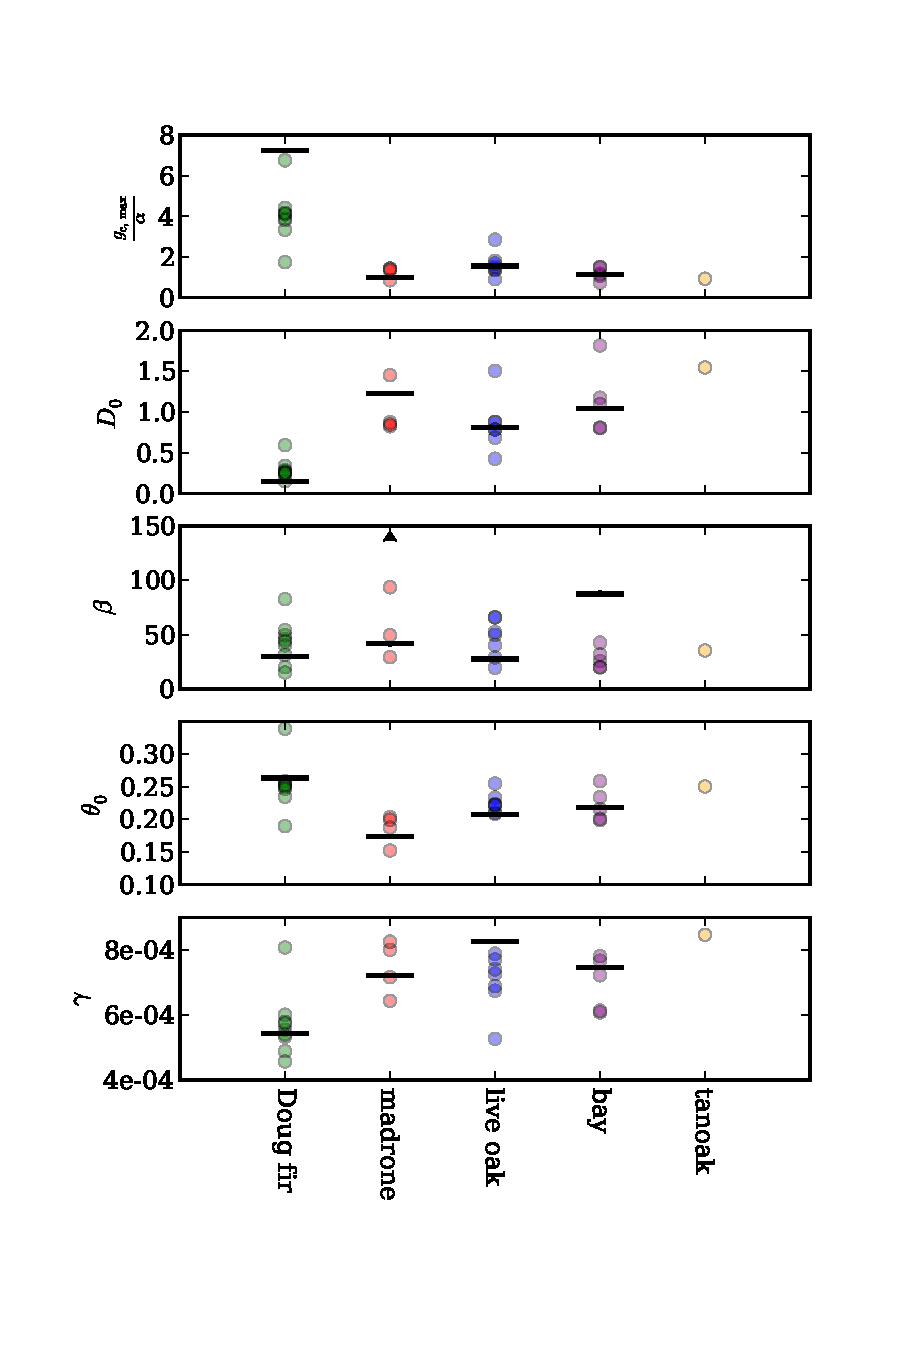
\includegraphics[width=0.65\textwidth]{ch1-sapflow/figures/Figure07.pdf}
\caption{Estimated Jarvis parameters, sorted by species.  Each circle represents the median of the posterior distribution for an individual sensor.  Black horizontal lines show the medians of the posterior distributions for the species-averaged timeseries parameters; vertical black error bars show the 95\% HPD interval (for most species-averaged timeseries parameters, this interval is smaller than the thickness of the horizontal line.)  Row 1: $g_{cmax}/\alpha$ parameter (kPa$^{-1}$), indicating sap velocity at low values of \textit{VPD} and radiation.  Row 2: $D_o$ parameter (kPa), which measures the curvature of the sap velocity increase with increasing \textit{VPD}.  Row 3: $\beta$ parameter (unitless), which measures the rate of sap flow decline around a soil moisture threshold.  The black triangle indicates that one madrone tree has a $\beta$ value higher than 150. Row 4: $\theta_0$ parameter (unitless), which measures the soil moisture value at which sap flow decline is centered.  Row 5: $\gamma$ parameter ((W/m$^2$)$^{-1}$), slope of the sap velocity increase with increasing radiation.}
\label{fig:sapflow_params}
\end{figure}

The Jarvis model parameters for all trees, separated by species, are shown in Figure \ref{fig:sapflow_params} and summarized in Table \ref{tbl:sapflow_mcmc}.  For 25 of the 26 trees, the posterior distributions of all five parameters are sharply peaked and well within the initial uniform prior chosen (example posterior distributions are shown in Figure \ref{fig:sapflow_posterior}).  One Pacific madrone tree (tree 16) has a broader distribution for $\beta$ than other trees (see 95\% HPD interval in Table \ref{tbl:sapflow_mcmc}.)

\begin{table}
  \caption{Median values of estimated Jarvis parameter distributions for each tree, with uncertainties calculated from the 
95\% HPD interval.}
  \label{tbl:sapflow_mcmc}
  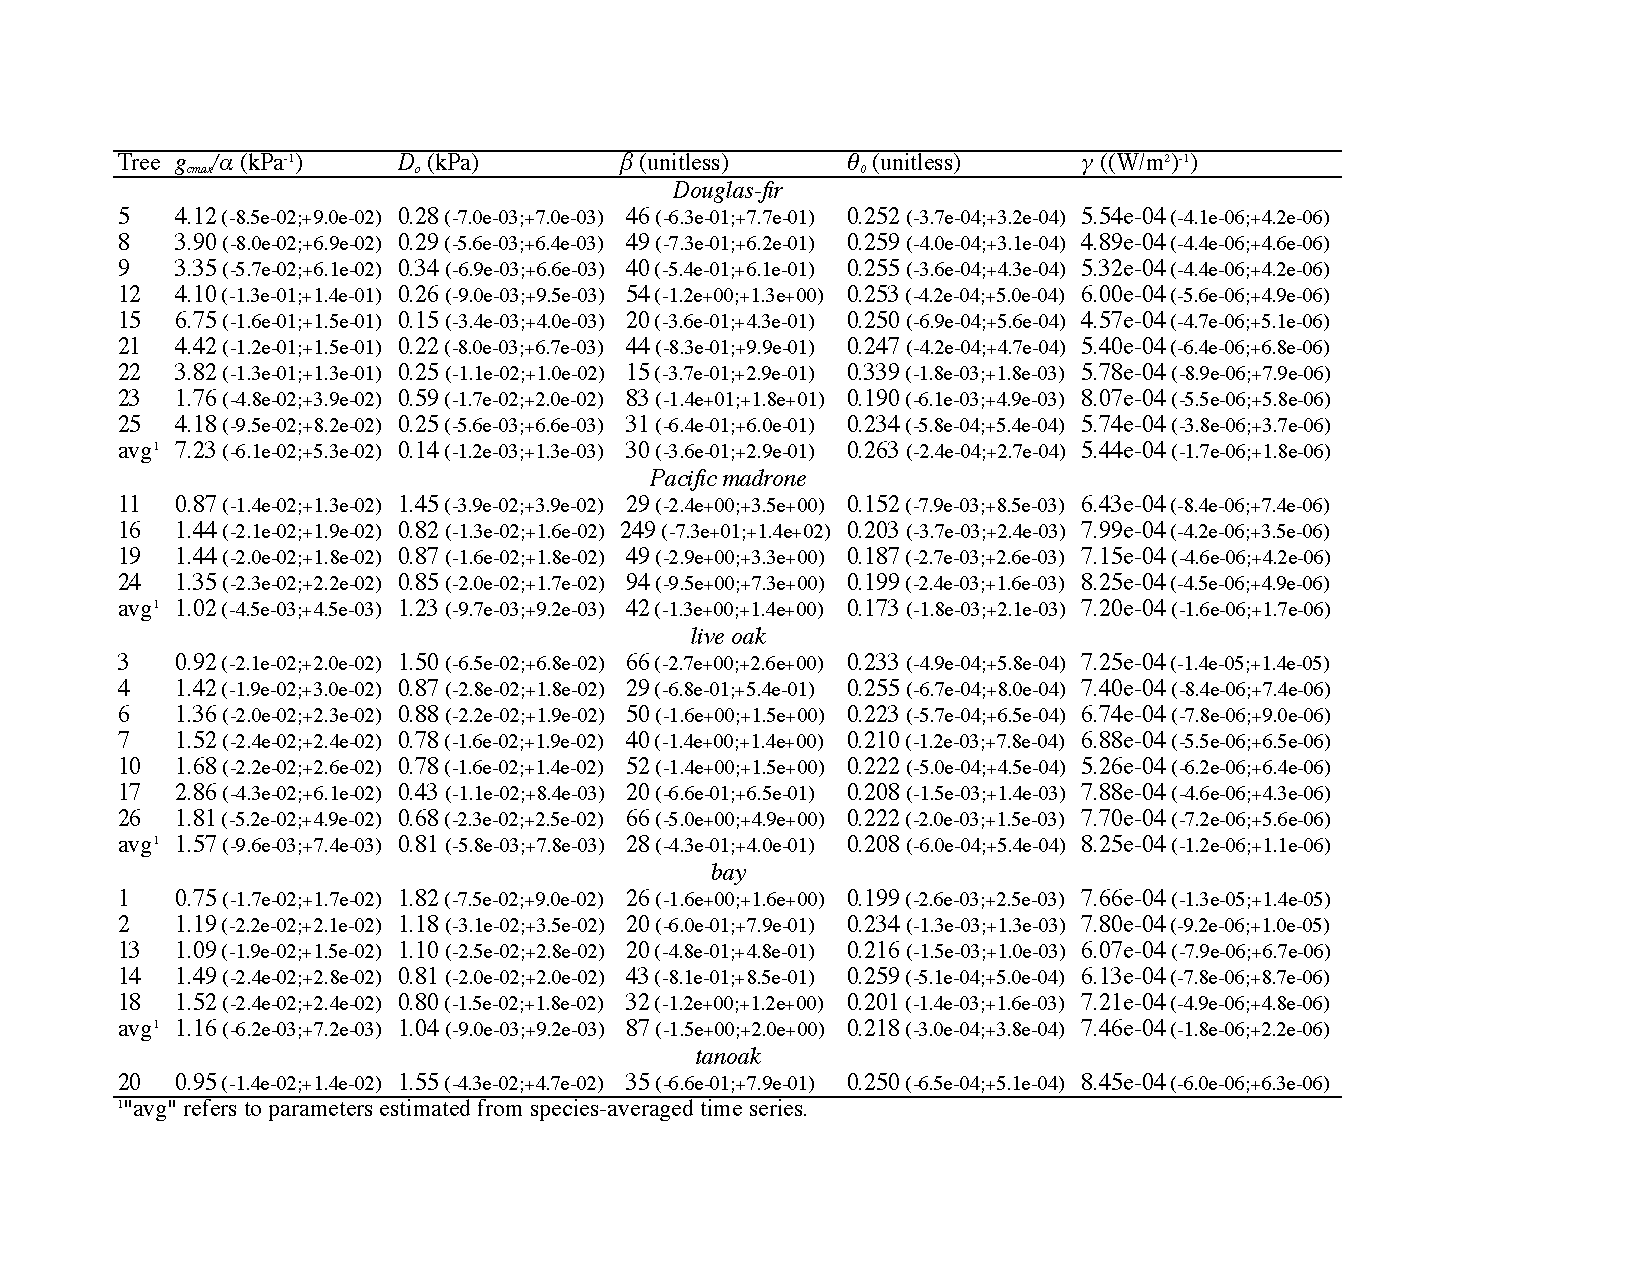
\includegraphics[width=\linewidth]{ch1-sapflow/tables/TableA2}
\end{table}

\begin{figure}[here]
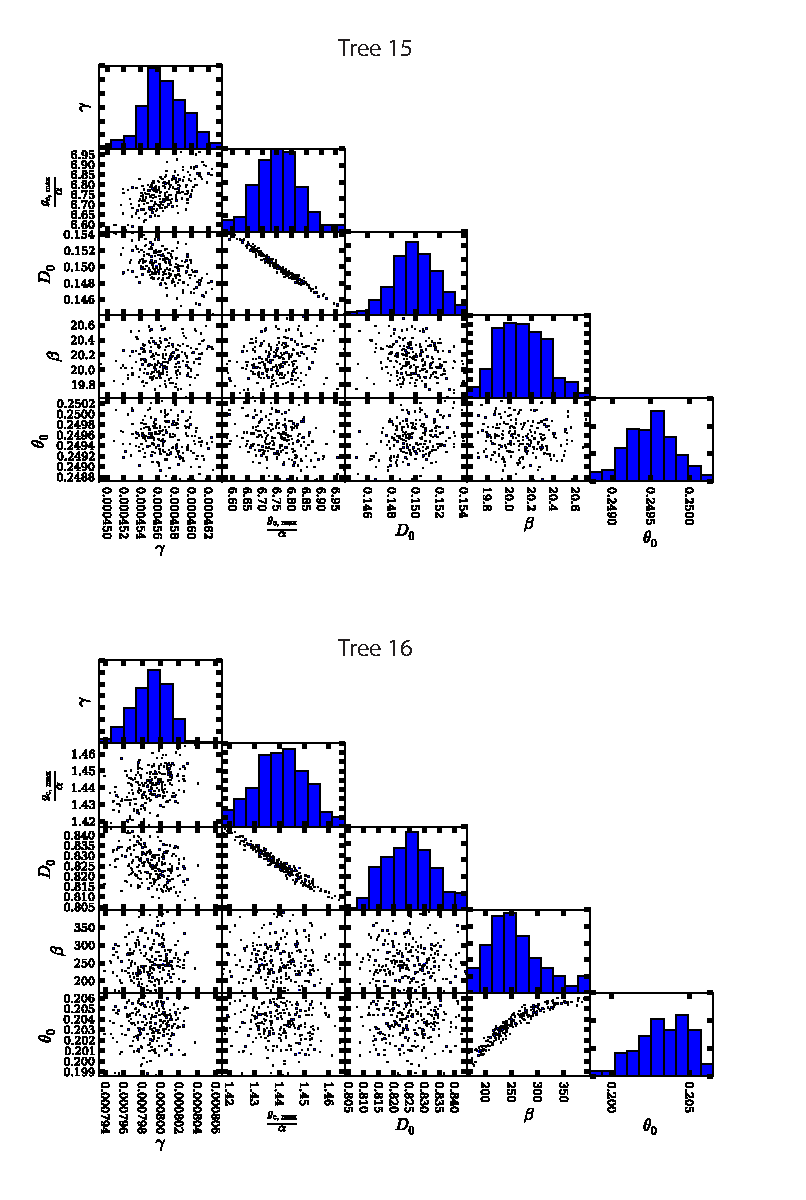
\includegraphics[width=0.75\textwidth]{ch1-sapflow/figures/FigureA1.pdf}
\caption{Panels on the diagonal: posterior distributions of environmental response parameters for the example Douglas-fir sensor (top) and the example Pacific madrone sensor (bottom.)  Panels below the diagonal: covariation of each pair of parameters for each example sensor.}
\label{fig:sapflow_posterior}
\end{figure}

The distributions of the median \textit{VPD} parameters for all sensors and for the species-averaged timeseries parameters ($g_{cmax}/\alpha$ and $D_o$, Figure \ref{fig:sapflow_params}, rows 1 and 2) confirm that sap flow in Douglas-firs across this site increases quickly at low \textit{VPD} and plateaus at high \textit{VPD} (high $g_{cmax}/\alpha$ and low $D_o$).  The broadleaf species, in contrast, respond more gradually with increasing \textit{VPD} (lower $g_{cmax}/\alpha$ and higher $D_o$).

The fitted soil moisture parameter $\theta_o$ (Figure \ref{fig:sapflow_params}, row 4) also shows a species difference.  Douglas-firs have higher $\theta_o$ values; their decline in response to soil moisture limitation is centered on a relative $\theta$ value of 0.263 (from species-averaged timeseries;  $-2.4 \times 10^{-4}$, $+2.7 \times 10^{-4}$ 95\% HPD interval).  Pacific madrones, on the other hand, have lower $\theta_o$ values when fitted to the sigmoid functional form, with declines centered on 0.173 (from species-averaged timeseries; $-1.8 \times 10^{-3}$, $+2.1 \times 10^{-3}$ 95\% HPD interval).

The parameter $\beta$ for individual sensors is more evenly distributed across species, indicating little species difference in the rate of sap flow decline below each individual tree's soil moisture threshold (Figure \ref{fig:sapflow_params}, row 3).  Pacific madrone sensors tend to have higher values of $\beta$, indicating that once their low $\theta_o$ is reached, their transpiration declines sharply; however, $\theta$ values below the Pacific madrone $\theta_o$ values were infrequently observed, so their decline is not well constrained.

The slopes $\gamma$ of the radiation function (Figure \ref{fig:sapflow_params}, row 5) range from $5 \times 10^{-4}$ to $8 \times 10^{-4}$ (W/m$^2$)$^{-1}$.  Douglas-firs tend to have lower slopes, indicating relatively high sap velocity at low \textit{I} and less sensitivity to \textit{I} increase.  In contrast, the broadleaf species (Pacific madrones, live oaks, and bays) have higher slopes, indicating that their sap velocity increases more with increasing \textit{I}.

In general, the parameters do not vary systematically by tree diameter or position on the slope.  There is some increase of $g_{cmax}/\alpha$ and decrease of $D_o$ with increasing tree diameter, but this effect is difficult to disentangle from species differences, because all trees larger than 60 cm in diameter are Douglas-firs, while many of the smaller trees are broadleaf species.  This lack of diameter- and position-dependence is consistent with the PCA results, which suggest that species differences represent the largest contribution to the observed sap flow variability.

The MCMC results show that Douglas-firs and Pacific madrones are at opposite ends of the spectrum of response to \textit{VPD} and $\theta$.  Douglas-firs increase sharply in response to \textit{VPD} and then plateau, while Pacific madrones increase gradually and continually with increasing \textit{VPD}.  Douglas-firs decline significantly at low $\theta$ values, while Pacific madrones show little to no suppression with low $\theta$ values.  Live oaks and bays fall between these end-member responses.

\subsection{Synoptic-scale temporal variability}

\begin{figure}[here]
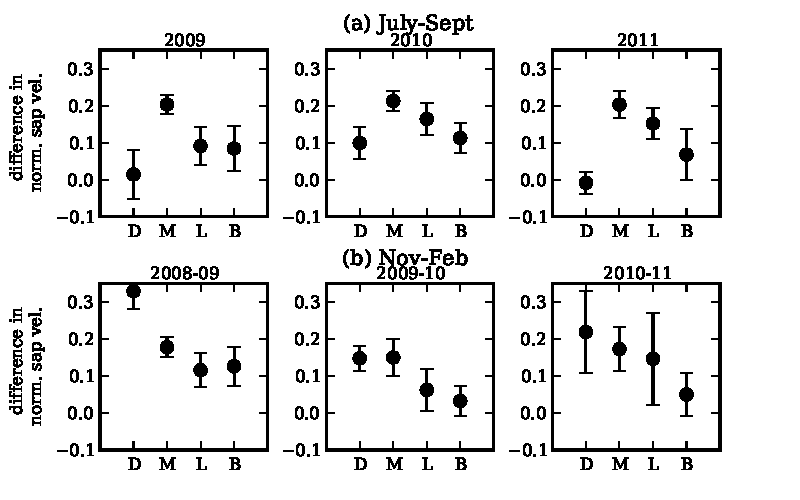
\includegraphics[width=0.9\textwidth]{ch1-sapflow/figures/Figure08.pdf}
\caption{Difference in normalized daily integral sap velocity between high \textit{VPD} days and low \textit{VPD} days, by species (D=Douglas fir, M=Pacific madrone, L=live oak, B=bay).  Circles show mean difference across all trees in the species for that season, and error bars show one standard deviation.  Row (a): July to September, where high \textit{VPD} days are days with maximum \textit{VPD}$>$2 kPa, and low \textit{VPD} days are days with maximum \textit{VPD}$<$2 kPa.  Row (b): November to February, where high \textit{VPD} days are days with maximum \textit{VPD}$>$0.5 kPa, and low \textit{VPD} days are days with maximum \textit{VPD}$<$0.5 kPa.}
\label{fig:sapflow_synoptic}
\end{figure}

The different sensitivity to \textit{VPD} in Douglas-firs and Pacific madrones translates to different transpiration response to synoptic-scale (daily to weekly, weather-scale) variability in atmospheric evaporative demand.  In the summer dry season, \textit{VPD} varies around a high seasonal mean, and the daily maximum value is seldom lower than 1.5 kPa (Figure \ref{fig:sapflow_abundances}(c)).  In this summer range of \textit{VPD} from 1.5 to more than 5 kPa, Douglas-firs have already reached their maximum sap velocity (Figure \ref{fig:sapflow_scatter}(a), for example), but the sap velocity of Pacific madrones, and to a lesser extent live oaks and bays, continues to increase with increasing \textit{VPD}.  Thus, Pacific madrone transpiration is expected to vary significantly in the dry season between high \textit{VPD} and low \textit{VPD} days, while Douglas-fir transpiration should not.  Figure \ref{fig:sapflow_synoptic}(a) shows the summer (July-September) average difference in normalized daily integral sap flow between high \textit{VPD} days (R3 daily max $>$2 kPa) and low \textit{VPD} days (R3 daily max $<$2 kPa) for each species.  Douglas-firs show little to no difference between high \textit{VPD} and low \textit{VPD} days in the summer, while Pacific madrones' sap flow is up to 0.2 normalized units (20\%) higher on high \textit{VPD} days than low \textit{VPD} days.

In the rainy winter, in contrast, \textit{VPD} varies around a much lower seasonal mean, so that the dynamic range of daily maximum \textit{VPD} is 0 to 2 kPa.  In this range, Douglas-firs are highly sensitive to \textit{VPD}, whereas Pacific madrones, live oaks, and bays are less sensitive.  Thus, in the wet winter season, Douglas-firs have greater variability in response to weather-scale \textit{VPD} variation.  Figure \ref{fig:sapflow_synoptic}(b) shows the winter (November-February) average difference in normalized daily integral sap flow between high \textit{VPD} days (R3 daily max $>$0.5 kPa) and low \textit{VPD} days (R3 daily max $<$0.5 kPa).  Douglas-fir sap flow is around 0.2 normalized units (20\%) higher on winter high \textit{VPD} days than low \textit{VPD} days.  Pacific madrones, live oaks, and bays also have higher sap flow on high \textit{VPD} days but by a lesser amount, 0.05-0.15 normalized units (5-15\%).

\subsection{Interannual variability}

\begin{figure}[here]
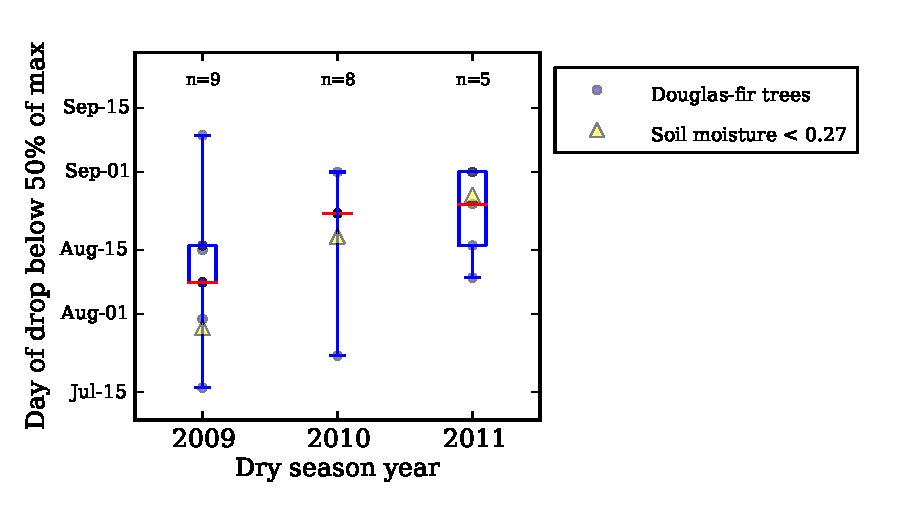
\includegraphics[width=0.9\textwidth]{ch1-sapflow/figures/Figure09.pdf}
\caption{Timing of dry season decline of Douglas-fir trees in each observation year. Each blue dot represents the date of decline below 50\% of a Douglas-fir tree�s maximum daily integral, using only high VPD days (R3 daily max $>$2.5 kPa, linearly interpolating across gaps). The box diagram for each year shows the quartiles of the distribution of all Douglas-fir sensors, with the red line indicating the median. The yellow triangles show the date that site-averaged relative $\theta$ declined below 0.27.}
\label{fig:sapflow_interannual}
\end{figure}

The timing of onset of Douglas-firs' dry season decline varies between years.  Figure \ref{fig:sapflow_interannual} shows the date in each dry season when each Douglas-fir sensor dropped below 50\% of its maximum daily integral, using only high \textit{VPD} days (R3 daily max $>$2.5 kPa, linearly interpolating across gaps), and the box diagrams show the quartiles of the distribution of all Douglas-fir sensors in each year.  The timing of the sap flow decline varies among the three years, occurring approximately two weeks earlier in 2009 than in 2010 or 2011.  The timing of soil moisture depletion also varies among the years, with depletion happening earliest in 2009 and latest in 2011 (yellow triangles in Figure \ref{fig:sapflow_interannual}), largely due to the timing of the last spring storm.  The date of relative soil moisture decline below 0.27 and the median date of Douglas-fir decline below 50\% are close in all three years, although there is notable scatter.

\subsection{Regional transpiration estimates}

\begin{figure}[here]
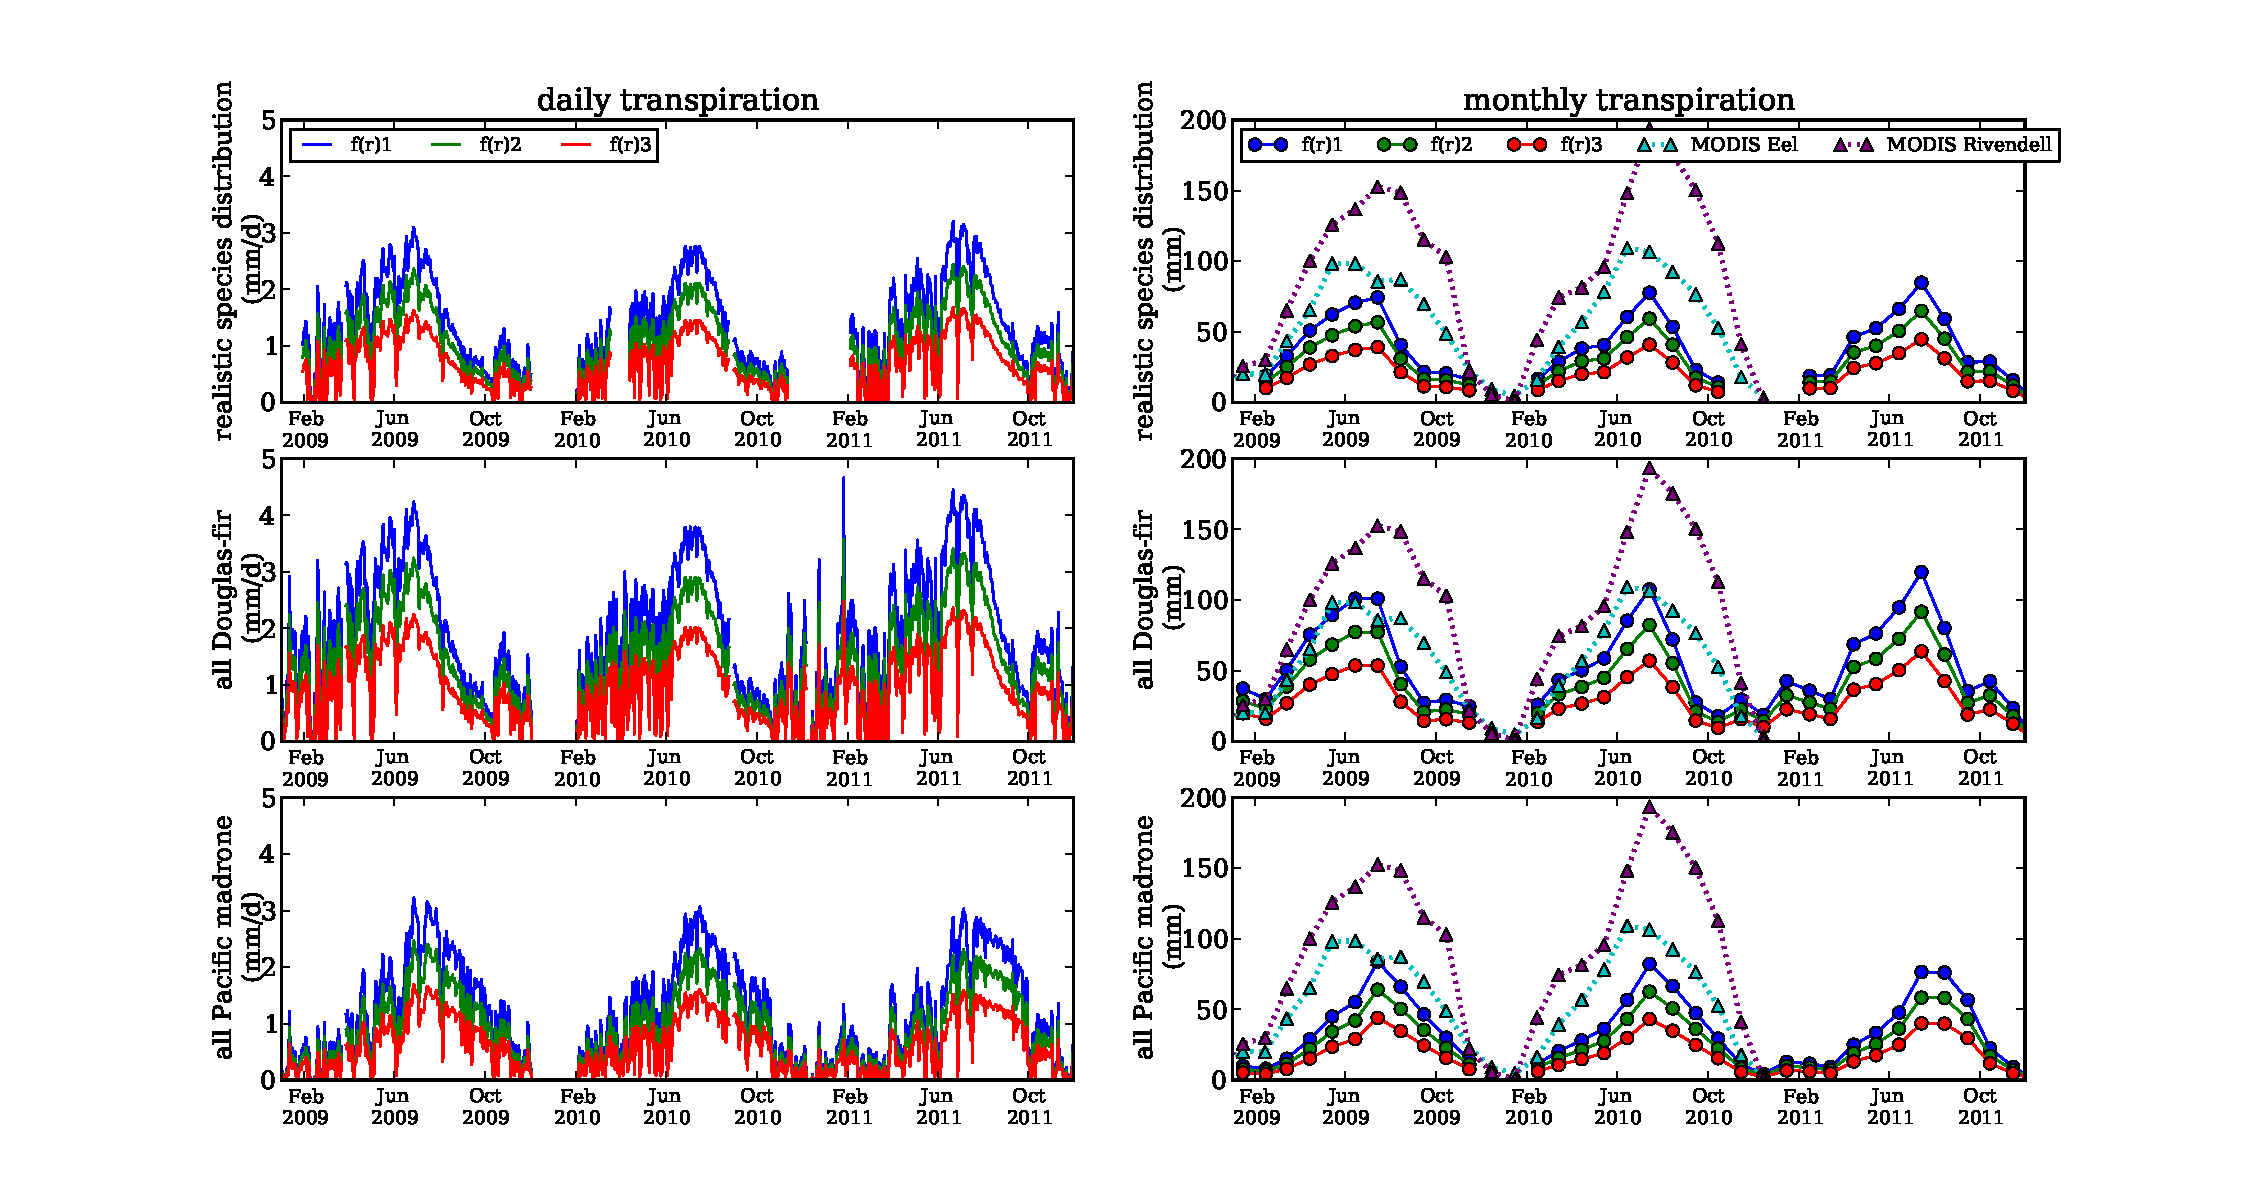
\includegraphics[width=0.9\textwidth]{ch1-sapflow/figures/Figure10.pdf}
\caption{Estimates of regional transpiration.  Left column: daily average transpiration rate estimated for the three plausible radial functions of sap velocity, using a realistic species distribution (top), assuming all trees are Douglas-fir (center), and assuming all trees are Pacific madrone (bottom.)  Right column: monthly integrals of transpiration estimates, again for the three plausible radial velocity profiles, and for the same three cases of species distribution.  Also shown in the right column are remote sensing estimates of monthly ET at two spatial scales: nearest MODIS pixel to the field site (purple), and MODIS estimate averaged over the Eel River watershed (cyan.)}
\label{fig:sapflow_regional}
\end{figure}

Our bottom-up estimates of regional transpiration, estimated with the aid of the FIA data, are shown at daily and monthly timescales in Figure \ref{fig:sapflow_regional} and are compared with a top-down remote sensing estimate of ET derived from MODIS through 2010 in Figure \ref{fig:sapflow_regional}, right column.  Our estimates using a realistic species distribution (row 1) show highest transpiration in June and July and a marked decline in the dry season.  The hypothetical all-Douglas-fir estimate (row 2) is very similar, which is not surprising because a large fraction of trees in the Eel watershed are Douglas-firs, redwoods, or other conifers, and thus the estimate in row 1 is strongly influenced by the Douglas-fir dynamics.  The all-Pacific-madrone hypothetical case (row 3), in contrast, has lower spring (February-May) transpiration and higher dry season (August and September) transpiration than either the realistic species distribution estimate or the all-Douglas-fir estimate.

The three radial sap velocity profiles tested give transpiration estimates that vary by approximately a factor of two.  The upper end of the range is similar in magnitude to the average of MODIS-derived ET for pixels in the Eel watershed (cyan in Figure \ref{fig:sapflow_regional}, right column.)  The sap-flow-based estimates are smaller than the MODIS-derived estimate of ET for the pixel nearest the Rivendell site (purple in Figure \ref{fig:sapflow_regional}, right column) by a factor of 2 to 3.

\begin{figure}[here]
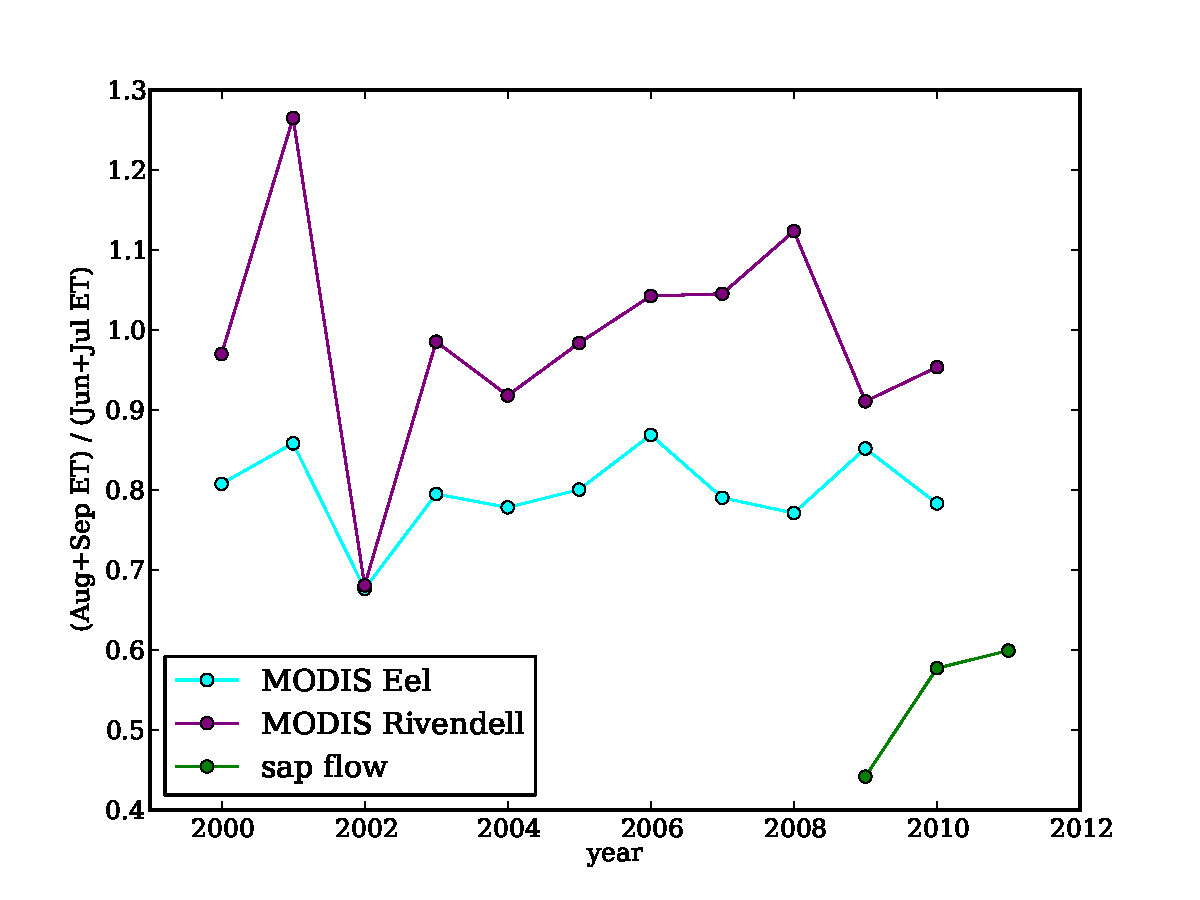
\includegraphics[width=0.9\textwidth]{ch1-sapflow/figures/Figure11.pdf}
\caption{Ratio of dry season to peak season ET (MODIS) or transpiration (sap flow); dry season is defined as August + September, and peak season is defined as June + July.  Two spatial scales are shown for MODIS: the pixel nearest to the Rivendell site (purple) and the average for all pixels in the Eel watershed (cyan.)}
\label{fig:sapflow_ratio}
\end{figure}

With the realistic species distribution, we estimate lower dry season (August-September) transpiration relative to peak (June-July) transpiration than does MODIS.  Figure \ref{fig:sapflow_ratio} shows August plus September transpiration divided by June plus July transpiration for MODIS-derived ET from 2000 to 2010, and for our estimates from 2009 to 2011.  In our estimates, the ratio of dry season transpiration to peak transpiration is the same regardless of radial sap velocity profile (the integral factor in Equation \ref{eqn:transpreg} cancels), so only one sap-flow-based estimate is shown in Figure \ref{fig:sapflow_ratio}.  The MODIS ratio of dry season transpiration to peak transpiration is close to 0.8 for the Eel watershed average and close to 1 for the near-Rivendell pixel for all years and is markedly higher than the sap-flow-based ratio, which is close to 0.5 in all three years.




\section{Discussion}

\subsection{Species difference in response to \textit{VPD} and $\theta$}
Evergreen tree species that coexist on this small hillslope transpire maximally during different seasons.  This difference in transpiration seasonality is due to the species-specific sensitivities of transpiration to atmospheric evaporative demand and subsurface water supply.  Douglas-fir transpiration reaches near-maximum values on clear-sky days in the rainy spring when relative soil moisture exceeds a threshold of $\sim$0.3 even when \textit{VPD} is low (around 1 kPa), and Douglas-fir transpiration declines sharply with the low surface soil moisture conditions of the dry summer.  In contrast, Pacific madrone, live oak, bay, and tanoak transpiration increases continually with increasing \textit{VPD}, reaching maximal transpiration values when atmospheric evaporative demand is highest in the summer dry season; in addition, the low moisture in the upper 50 cm of soil in the summer dry season does not suppress Pacific madrone transpiration and suppresses the other broadleaf species to a lesser degree than it does Douglas-fir.  As a result, Douglas-firs have highest transpiration on clear days in spring, while broadleaf species, and especially Pacific madrones, have highest transpiration on summer days with high atmospheric demand (Figure 4).  The Douglas-fir seasonal pattern is consistent with other studies [\textit{Jassal et al.}, 2009; \textit{Moore et al.}, 2004; \textit{Granier}, 1987]; no studies of Pacific madrone transpiration seasonal patterns were found in the literature.

Sensitivity to \textit{I} also differed between Douglas-firs and the broadleaf species: broadleaf transpiration showed a greater relative increase with increasing \textit{I} than did Douglas-fir transpiration. This species difference might arise in part because, although the parameters are estimated with open-field \textit{I}, trees of different heights on this north-facing slope actually have different access to \textit{I}. Large Douglas-firs (up to 50-60 m tall) generally have greater \textit{I} access than understorey broadleaf trees (20-30 m tall).  Thus, during low \textit{I} times such as mornings or winter days, the large Douglas-firs might have sufficient \textit{I} for photosynthesis and transpiration, while understorey trees might not.

\subsection{Species difference in water access}
It remains uncertain how the broadleaf species and especially Pacific madrones, unlike Douglas-firs, are able to maintain high rates of transpiration during the summer dry period. In order to maintain these high transpiration rates, Pacific madrones must rely either on a more readily available source of water (by placing roots in areas with more moisture, e.g. deeper, or in areas that have higher hydraulic conductivity), or on more-tightly-bound water (by maintaining hydraulic function at lower xylem and leaf water potentials).  There is evidence that Pacific madrones may use both of these mechanisms: at a similar site in southwest Oregon, Douglas-fir roots were confined mainly to the upper 1.5 m of the subsurface, with no roots found below 2.5 m, while Pacific madrones in the same area had notably deeper roots, extending to 2-3.5 m below the surface into rock fissures [\textit{Wang et al.}, 1995; \textit{Zwieniecki and Newton}, 1995;  \textit{Zwieniecki and Newton}, 1996], and Pacific madrones at the Oregon site used water across a greater depth than Douglas-firs [\textit{Zwieniecki and Newton}, 1996].  Moisture in weathered rock can be an important plant water source [\textit{Schwinning}, 2010; \textit{Schwinning}, 2013], and the saprolite zone at our site has significant seasonal variation in water storage and could be an important source for some or all species here [\textit{Salve et al.}, 2012].  Additionally, previous research has shown that Pacific madrones have minimum leaf water potentials of about -3.0 MPa [\textit{Morrow and Mooney}, 1974; \textit{Wang et al.}, 1995], vs. -2.0 MPa in Douglas-firs [\textit{Running}, 1976; \textit{Wang et al.}, 1995]; Pacific madrones' lower minimum leaf water potential suggests that Pacific madrones are less vulnerable to hydraulic failure as soil moisture declines [\textit{Choat et al.}, 2012] and thus might be able to access water bound at low matric potential that is inaccessible to Douglas-fir. Our aboveground sap flow observations cannot distinguish between these two possible mechanisms of water access, but other researchers are using stable isotopes to investigate the water sources for different trees at the site [\textit{Oshun et al.}, 2012], and preliminary results suggest that needleleaf species and broadleaf species use isotopically distinct water sources within the unsaturated zone.  Thus, Douglas-fir (sensitive stomatal control, shallow rooted, and vulnerable to hydraulic failure) and Pacific madrone (less sensitive stomatal control, deeper rooted, and less vulnerable to hydraulic failure) employ contrasting stomatal strategies that are logically connected to hydraulic vulnerability and rooting depth.

We speculate that Pacific madrones may also have higher leaf area during the summer.  Pacific madrone leaves have a lifespan of 14.7 months [\textit{Ackerly}, 2004], meaning that if new leaves emerge at approximately the same time, then for a two- to three-month period each year, the trees might have twice their normal leaf area.  Informal observations at our site indicate that Pacific madrones drop leaves in late summer, so mid-summer may be the high-leaf-area period.  When the leaf area is higher, whole tree transpiration could increase even if transpiration per leaf stayed the same or declined, provided that water stress were not extreme.

Interestingly, Douglas-fir trees at our site do not seem to use groundwater to alleviate water stress during the dry season.  Tree 5, a large Douglas-fir downslope where the water table is $\sim$5 m below ground year-round, declined at a similar rate to upslope Douglas-firs in the dry season (similar soil moisture parameters in Table A2).  Like the instrumented upslope Douglas-firs, tree 5 rebounded strongly with the onset of the rainy season, suggesting water limitation during the dry season until unsaturated zone moisture was replenished by rains.

\subsection{Implications of Douglas-fir water stress}
Douglas-firs' sap flow declined through the dry season in all three years, but the timing of onset of the decline varied between years, corresponding to the timing of moisture decline in the top 50 cm of soil (Figure 9).  The timing of surface soil moisture decline, in turn, seems to depend on the timing of late spring precipitation (Figure 3).  Excess rain during the winter and early spring that exceeds the storage capacity of the soil will run off and have little influence on summer soil moisture availability, but rain in the late spring has the potential to refill a partially empty upper soil reservoir and sustain soil moisture further into the dry season.  Thus, the timing of late spring precipitation is important for sustaining Douglas-fir transpiration through the dry season.  As long as late spring storms meet a certain threshold quantity, their timing may matter more than total wet season precipitation for Douglas-fir function in the dry season.

Douglas-firs may be encroaching on areas formerly dominated by Pacific madrone and other broadleafs in the ACRR, due to a fire-regime shift from controlled burning by indigenous people and early European settlers, to fire suppression in the 20th century [\textit{Johnson}, 1979].  If Douglas-firs become more prevalent, their suppressed transpiration in the dry season could decrease the regional summertime evapotranspiration (Figure 10) and might increase the land surface temperature in the dry season [\textit{Link et al.}, in preparation].  California Coast Range forests with a greater proportion of Douglas fir might also be less resilient to drought, if the Douglas-firs' decline in stomatal conductance reduced whole-tree carbon balance and thus increased sensitivity to subsequent drought events [\textit{McDowell et al.}, 2008].

\subsection{Comparison with previous observations}
Our bottom-up estimate of transpiration agrees generally with the MODIS-derived top-down estimates at the scale of the Eel River watershed (Figure 10).  However, there are important differences in the dry season: we estimate notably lower transpiration in August and September than does the MODIS remote sensing method (Figure 11).  It is unlikely that the difference could be due to soil evaporation unaccounted for in the sap flow method, because surface soils are very dry in the late dry season.  It is possible that other conifer species in the watershed, such as redwood and pine species, have less stomatal closure than Douglas-fir at low soil moisture values, and that our method underestimates transpiration by these other species.  However, \textit{Pinaceae} tend to use water conservatively because they are vulnerable to embolism [\textit{Mart\'inez-Vilalta et al.}, 2004], suggesting that pine species in this region, which make up much of the ``other conifer'' category in Figure 4, would be likely to close their stomata under dry soil conditions like Douglas-firs do.  It is also possible that the FIA inventory underestimates the contribution of broadleaf species like Pacific madrone that transpire heavily in the dry season.  Certainly, broadleaf evergreens dominate transpiration locally on certain hillslopes: the species distribution is highly spatially patterned in the Elder Creek and Eel River watersheds, with broadleaf evergreen trees predominant on south-facing slopes and ridges, and Douglas-firs predominant on north-facing slopes and in valleys [Collin Bode and William Dietrich, personal communication].  As such, south-facing slopes may have higher dry season transpiration than north-facing slopes, creating structured spatial variability in dry season transpiration.  Finally, the MODIS algorithm, which uses remotely sensed LAI and reanalysis meteorology to drive a Penman-Monteith model [\textit{Mu et al.}, 2007], may not accurately account for Douglas-fir stomatal closure when soils are dry, because the MODIS algorithm does not incorporate soil moisture information.  Comparison with ET measured by flux towers suggests that the MODIS-derived annual cycle of ET for Mediterranean sites contains large errors [\textit{Vinukollu et al.}, 2011; one flux tower located in the Sierra Nevada foothills oak savanna and one on the western slope of the Sierra Nevada in a mixed-evergreen coniferous forest].

We note that our estimates also agree with measurements of similar sites made with a variety of methods.  \textit{Salve et al.} [2012] used a water balance to calculate an annual ET at Rivendell (excluding interception losses) of 300-500 mm and summer (June-September) ET  of up to 200 mm.  Our estimate using the realistic species distribution and the first radial velocity profile (blue line in Figure 10, top row) gives annual transpiration of 350-410 mm and June-September transpiration of 150-180 mm.  At a wetter Douglas-fir site in British Columbia using the eddy flux method, \textit{Jassal et al.} [2009] measured similar spring and early summer monthly ET (50-70 mm/month), although late summer ET was greater at the wetter British Columbia site than at Rivendell.  At a Douglas-fir site in western Oregon, \textit{Moore et al.} [2004] used sap flow scaling to estimate Douglas-fir dry season transpiration of 0.5-2.5 mm/day, depending on tree age and time within the dry season; these rates bracket our dry season estimates (top left panel of Figure 10.)  In addition, measurements of oak transpiration at a Mediterranean site agree with the oak sap velocities we measured (\textit{Fisher et al.} [2007] measured peak sap velocities around 6 cm/hr) and the transpiration rates we estimate (\textit{Chen et al.} [2008] report oak tree transpiration of 2-4 mm/day in early- to mid-summer.)

\subsection{Uncertainties and limitations}

\subsubsection{Soil moisture}
In this study, we aggregate measurements of soil moisture from across the hillslope into a single site average.  A spatial pattern in $\theta$ has been observed at this site, with downslope profiles maintaining higher moisture content longer into the dry season [\textit{Salve et al.}, 2012].  However, we choose to compare sap flow to a single, site-averaged value of soil moisture for two reasons: (1) a moisture content--matric potential calibration has not been performed, and the variation of material properties along the slope means that the spatial pattern of moisture content might not directly translate to a spatial pattern of matric potential; (2) the location of roots is uncertain, especially for large trees, which, on this steep slope, have root systems extending great lateral distances and deeply into the hillside, and it is thus difficult to constrain where trees are accessing water (i.e., we cannot weight our average by root density [\textit{Chen et al.}, 2008]).  Thus, we use a single averaged relative $\theta$ as an index of water availability, with the recognition that it imperfectly represents the water available to each individual tree.

The TDR measurements of the top 50 to 70 cm do not measure the water content of the saprolite zone between 1 and 3 m below the surface, which may be an important reservoir of plant-available moisture [\textit{Salve et al.}, 2012].  Unfortunately, the measurements used by \textit{Salve et al.} [2012] to explore the saprolite moisture dynamics are not suited to our analyses in this study because of as-yet-undetermined calibration to moisture content (ERSAS) or low temporal resolution (neutron probe).  We compare tree water use to surface (top 50 to 70 cm) soil moisture because it is readily measured at present; as techniques for quantifying moisture in saprolite and weathered rock advance, tree water use should be compared to those observations as well.

\subsubsection{Sap velocity vs. transpiration}
In treating sap velocity as proportional to transpiration, we assume that (1) the radial profile of sap velocity in the sapwood is constant in time, and (2) the change in storage between the measurement point and the leaves is small.  The first assumption is a reasonable [\textit{Cohen et al.}, 1985; \textit{Nadezhdina et al.}, 2002; \textit{Dragoni et al.}, 2009] but not perfect [\textit{Ford et al.}, 2004] approximation.  The second assumption introduces more error at sub-diurnal timescales, when storage changes and temporal lags in velocity between stem and leaf can be significant [e.g. \textit{Waring and Running}, 1978; \textit{Buckley et al.}, 2011], but in the daily integral, the storage change is less than 5\% in Douglas-fir [\textit{Waring and Running}, 1978]; the daily storage change in other species varies but also tends to be small (negligible in \textit{Larix} and \textit{Picea} [\textit{Schulze et al.}, 1985], and up to 3\% in \textit{Juglans regia} [\textit{Constantz and Murphy}, 1990]).  We neglect this storage contribution to transpiration for simplicity.

Similarly, in converting heat pulse velocity to sap velocity, we treat xylem water content as constant through the year, but xylem water content, especially in Douglas-fir [\textit{Waring and Running}, 1978], may decline during long dry periods.  Our water content measurements were made at the end of the dry season and were thus probably a lower bound.  According to Equation 7 in \textit{Burgess et al.} [2001], an underestimation of water content in the wet season would result in an underestimation of sap velocity during the wet season.

\subsubsection{Regional estimate of transpiration}
We have estimated regional transpiration in order to demonstrate the potential for species differences in response to $VPD$ and $\theta$ to influence transpiration at a regional scale.  The estimate required several simplifying assumptions.  First, species recorded in the FIA dataset were grouped into broad categories of needleleaf and broadleaf, both in order to estimate the maximum potential impact of Pacific-madrone-like behavior in broadleafs and also to accommodate species not measured at the Rivendell site.  This coarse categorization could and should be improved if additional species (especially the common conifers) are instrumented in the future.  Second, the sapwood thickness - DBH relationship is poorly constrained for species other than Douglas-fir (our Pacific madrone relationship was based on only 6 samples, and samples were not collected from other broadleaf species at the site because the hardness of the wood made it prohibitively difficult with the available equipment).  This allometric relationship is expected to vary between sites, species, and trees of different ages [\textit{Eamus et al.}, 2006, p. 42]; as such, this relationship is a significant source of uncertainty in our regional estimate.  Similarly, the radial profile of sap velocity is another significant source of uncertainty, and we attempt to quantify this uncertainty by producing three regional estimates, using three reasonable radial velocity profiles (Figure 10.)  However, any errors due to sapwood thickness and radial velocity profile would not change the seasonality of the transpiration estimates, only the magnitude.

Finally, in using small-scale measurements to estimate the behavior of trees at the regional scale, we neglect heterogeneity among hillslopes.  Our regional estimate does not account for heterogeneous meteorology and water availability, or for variation in response between trees in different locations due to, for instance, genetics, climate during growth, or age distribution.  More sap flow and micrometeorological measurements at different sites within the Eel River watershed, as well remotely sensed observations of vegetation, could integrate such heterogeneity and improve the accuracy of the regional estimate.



\section{Conclusions}
Two evergreen tree species common to forests of the northern Pacific US coast have different seasons of peak transpiration, due to their different responses to atmospheric evaporative demand and soil water limitation.  Douglas-fir transpiration is phase-shifted from the annual cycle of solar radiation toward an earlier season of transpiration, with higher transpiration in the wet spring; this is because Douglas-firs' stomatal conductance is sensitive to water availability and \textit{VPD} and their transpiration thus declines through the dry season.  Pacific madrone transpiration, in contrast, is phase-shifted toward a later season of transpiration, with higher transpiration in the dry summer; this is because broadleaf tree species at this site, especially Pacific madrones, are less sensitive to water stress and maintain greater stomatal conductance at high \textit{VPD}.

The observations of sap flow were combined with a regional forest inventory to construct a bottom-up estimate of regional transpiration.  This estimate highlights the regional-scale impact of needleleaf evergreen stomatal sensitivity to water stress.  The resulting suppression of dry season transpiration could create feedbacks from the forest to atmospheric temperature and humidity, and the nature of these feedbacks would depend on species distribution [\textit{Link et al.}, in preparation].  Better constraints on historical and future changes in Pacific coast forest species composition are needed in order to understand the resulting impacts on the land-atmosphere exchange of water and energy.


\section*{Acknowledgments}

COAUTHORS; and mention WRR publication here?

We thank Daniella Rempe, William Dietrich, and Collin Bode for helpful comments and discussion.  The W. M. Keck Foundation provided support for the instruments used in this study.  Percy Link was supported by DOE grant DE-SC0001470 and NSF grant ATM-0628678.  Jasper Oshun was supported by NSF CMG Collaborative Research grant 0934818.

\section{Appendix: Markov Chain Monte Carlo}
\label{sec:sapflow_appendix}

The MCMC method we adopt computes the likelihood function, assuming that the sap flow measurement errors are normally distributed, and uses the Metropolis-Hastings algorithm to select new members of the chain from a proposal distribution [e.g., \textit{Sivia} 2006 XXXX]. We used the python PyMC module to execute this analysis [\cite{patil}]. The standard deviation of the measurement error for each sensor was determined from the noise floor of the sensor's power spectrum, using Parseval's theorem; the standard deviation for most sensors was 1-3\%, and the largest standard deviation was 8\%.  The Metropolis-Hastings algorithm guarantees convergence of the Markov chains, but convergence is slow when a high rate of rejection ($>>$50\%) of the proposed values occurs, a common circumstance for problems with a large number of parameters.  We investigated marginalization over errors in the environmental variables (temperature, relative humidity, radiation, and soil moisture) adopting a single test sensor for which this problem was computational tractable.  The most likely parameter values for this test sensor were slightly different from those derived assuming the environmental parameters are perfectly known, but the differences were small compared to the differences between sensors and compared to the range of the parameter space.  The 95\% confidence intervals did not widen noticeably in this test, but the slight differences in median values suggest that the 95\% confidence intervals quoted here underestimate the parameter uncertainties by up to a factor of 3.  However, all parameter distribution widths remained a small fraction of the spread in most likely parameters values derived for each species as a whole.  Thus, while the confidence intervals listed in Table \ref{tbl:sapflow_mcmc} should be viewed as lower limits to the true error for a given tree's parameters, we do not expect unaccounted-for uncertainties in environmental variables to significantly impact our species-wide conclusions.

\begin{table}
  \caption{Limits of uniform prior distributions for Markov chain Monte Carlo estimation of Jarvis model parameters (Equation \ref{eqn:sapflow_jarvis}.)}
  \label{tbl:sapflow_priors}
  \begin{tabular}{l r r}
  \hline
  Parameter & Lower limit & Upper limit \\
  \hline
  $g_{cmax}/\alpha$ (kPa-1) & 0 & 9 \\
  $D_o$ (kPa) & 0 & 2 \\
  $\beta$ (unitless) & 0 & 400 \\
  $\theta_0$ (unitless) & 0 & 0.35 \\
  $\gamma$ ((W/m$^2$)$^{-1}$) & 3x10$^{-4}$ & 9x10$^{-4}$ \\
  \hline
  \end{tabular}
\end{table}

We adopt uniform priors for the proposal distributions of the unknowns, and each chain is initialized with a random value within the prior range.  The adopted priors for the free parameters are given in Table \ref{tbl:sapflow_priors}, and we imposed them after exploration of the full range of parameters.  Following an initial ``burn in" period, we establish convergence and independence following \cite{raftery}.  Figure \ref{fig:sapflow_posterior} shows typical results from this analysis for two example trees.  For both trees, $\frac{g_{\rm c,\,max}}{\alpha}$ and $D_o$ are correlated, consistent with the results of \cite{oren1999survey}; $R^2$ values for $\frac{g_{\rm c,\,max}}{\alpha}$ -- $D_o$ correlation ranged from 0.92 to 0.99 over all trees.  For most madrone trees, $\beta$ and $\theta_0$ covary in a nonlinear way, as shown in Figure \ref{fig:sapflow_posterior} (Tree 16); $\beta$ and $\theta_0$ did not covary in this way for other species.  Other parameters are minimally correlated, and the degree of parameter independence shown in Figure \ref{fig:sapflow_posterior} is typical for all sensors.


%\section*{References}

\bibitem[{\textit{Ackerly}(2004)}]{Ackerly}
Ackerly, D. (2004), Functional strategies of chaparral shrubs in relation to seasonal water deficit and disturbance, 
\textit{Ecol. Monogr.}, \textit{74}(1), 25--44.

\bibitem[{\textit{Aranda}(2000)}]{Aranda}
Aranda, I., L. Gil, and J.~A. Pardos (2000), Water relations and gas exchange in \textit{Fagus sylvatica} L. and \textit{Quercus petraea} (Mattuschka) Liebl. in a mixed stand at their southern limit of distribution in Europe,
\textit{Trees}, \textit{14}, 344--352.

\textit{BALDOCCHI AND XU}

\bibitem[{\textit{Baquedano}(2004)}]{Baquedano}
Baquedano, F.~J., and F.~J. Castillo (2006), Comparative ecophysiological effects of drought on seedlings of the Mediterranean water-saver \textit{Pinus halepensis} and water-spenders \textit{Quercus coccifera} and \textit{Quercus ilex}, 
\textit{Trees}, \textit{20}, 689--700.

\bibitem[{\textit{Black}(1979)}]{Black}
Black, T.~A. (1979), Evapotranspiration from Douglas fir stands exposed to soil water deficits, 
\textit{Water Resour. Res.}, \textit{15}(1), 164--170.

\textbf{BONAN}

\bibitem[{\textit{Bond and Kavanagh}(1999)}]{Bond}
Bond, B.~J., and K.~L. Kavanagh (1999), Stomatal behavior of four woody species in relation to leaf-specific hydraulic conductance and threshold water potential,
\textit{Tree Physiol.}, \textit{19}, 503--510.

\bibitem[{\textit{Brooks}(2006)}]{Brooks}
Brooks, J.~R., F.~C. Meinzer, J.~M. Warren, J.-C. Domec, and R. Coulombe (2006), Hydraulic redistribution in a Douglas-fir forest: lessons from
system manipulations, \textit{Plant, Cell and Environment}, \textit{29}, 138--150.

\bibitem[{\textit{Buckley et al.}(2011)}]{Buckley}
Buckley, T.~N., T.~L. Turnbull, S. Pfautsch, and M.~A. Adams (2011), Nocturnal water loss in mature subalpine \textit{Eucalyptus
delegatensis} tall open forests and adjacent \textit{E. pauciflora}
woodlands, \textit{Ecology and Evolution}, 435--450.

\bibitem[{\textit{Burgess et~al.}(2001)}]{Burgess}
Burgess, S.~S.~O., M.~A. Adams, N.~C. Turner, C.~R. Beverly, C.~K. Ong, A.~A.~H. Khan, and T.~M. Bleby (2001), An improved heat pulse method to measure low and reverse rates of sap flow in woody plants, 
\textit{Tree Physiol.}, \textit{21}, 589--598.

\bibitem[{\textit{\v{C}erm\'{a}k et~al.}(1992)}]{Cermak}
\v{C}erm\'{a}k, J., E. Cienciala, J. Ku\v{c}era, and J.-E. H\"{a}llgren (1992), Radial velocity profiles of water flow in trunks of Norway spruce and oak and the response of spruce to severing, 
\textit{Tree Physiol.}, \textit{10}, 367--380.

\bibitem[{\textit{Chen}(2008)}]{Chen}
Chen, X., Y. Rubin, S. Ma, and D. Baldocchi (2008), Observations and stochastic modeling of soil moisture control on evapotranspiration in a Californian oak savanna,
\textit{Water Resour. Res.}, \textit{44}.

\bibitem[{\textit{Chirino}(2011)}]{Chirino}
Chirino, E., J. Bellot, and J.~R. S\'anchez (2011), Daily sap flow rate as an indicator of drought avoidance mechanisms in five Mediterranean perennial species in semi-arid southeastern Spain,
\textit{Trees}, \textit{25}, 593--606.

\bibitem[{\textit{Choat et~al.}(2012)}]{Choat}
Choat, B., S. Jansen, T.~J. Bodribb, H. Cochard, S. Delzon, R. Bhaskar, S. Bucci, T.~S. Feild, S.~M. Gleason, U.~G. Hacke, A.~L. Jacobsen, F. Lens, H. Maherali, J. Mart\'{i}nez-Vilalta, S. Mayr, M. Mencuccini, P.~J. Mitchell, A. Nardini, J. Pittermann, R.~B. Pratt, J.~S. Sperry, M. Westoby, I.~J. Wright, and A.~E. Zanne (2012), Global convergence in the vulnerability of forests to drought, 
\textit{Nature}, \textit{491}, 752--756.

\bibitem[{\textit{Cohen et~al.}(1985)}]{Cohen}
Cohen, Y., F.~M. Kelliher, and T.~A. Black (1985), Determination of sap flow in Douglas-fir trees using the heat pulse technique, 
\textit{Can. J. For. Res.}, \textit{15}, 422--428.

\textbf{CONSTANTZ AND MURPHY}

\bibitem[{\textit{Dang et~al.}(1997)}]{Dang}
Dang, Q.-L., H.~A. Margolis, M.~R. Coyea, M. Sy, and G.~J. Collatz (1997), Regulation of branch-level gas exchange of boreal trees: roles of shoot water potential and vapor pressure difference, 
\textit{Tree Physiol.}, \textit{17}, 521--535.

\bibitem[{\textit{David}}]{David}
David, T.~S., M.~O. Henriques, C. Kurz-Besson, J. Nunes, F. Valente, M. Vaz, J.~S. Pereira, R. Siegwolf, M.~M. Chaves, L.~C. Gazarini, and J.~S. David (2007), Water-use strategies in two co-occurring Mediterranean evergreen oaks: surviving the summer drought,
\textit{Tree Physiol.}, \textit{27}, 793--803.

\bibitem[{\textit{Dragoni}}]{Dragoni}
Dragoni, D., K.~K. Caylor, H.~P. Schmid (2009), Decoupling structural and environmental determinants of sap velocity, Part II. Observational application,
\textit{Agricultural and Forest Meteorology}, \textit{149}, 570--581.

\bibitem[{\textit{Feddes}}]{Feddes}
Feddes, R., P. Kowalik, and H. Zaradny (1978), \textit{Simulation of Field Water Use and Crop Yield}, John Wiley, New York.

\bibitem[{\textit{Ford et~al.}(2004)}]{Ford}
Ford, C.~R., M.~A. McGuire, R.~J. Mitchell, and R.~O. Teskey (2004), Assessing variation in the radial profile of sap flux density in \textit{Pinus} species and its effect on daily water use,
\textit{Tree Physiol.}, \textit{24}, 241--249.

\bibitem[{\textit{Franks}(2007)}]{Franks}
Franks, P.~J., P.~L. Drake, and R.~H. Froend (2007), Anisohydric but isohydrodynamic: seasonally constant plant water potential gradient explained by a stomatal control mechanism incorporating variable plant hydraulic conductance,
\textit{Plant, Cell and Environment}, \textit{30}, 19--30.

\bibitem[{GLOBE}]{GLOBE}
GLOBE Task Team and others (Hastings, D.~A., P.~K. Dunbar, G.~M. Elphingstone, M. Bootz, H. Murakami, H. Maruyama, H. Masaharu, P. Holland, J. Payne, N.~A. Bryant, T.~L. Logan, J.-P. Muller, G. Schreier, and J.~S. MacDonald), eds. (1999), The Global Land One-kilometer Base Elevation (GLOBE) Digital Elevation Model, Version 1.0. National Oceanic and Atmospheric Administration, National Geophysical Data Center, 325 Broadway, Boulder, Colorado 80303, U.S.A. Digital data base on the World Wide Web (URL: http://www.ngdc.noaa.gov/mgg/topo/globe.html) and CD-ROMs.

\bibitem[{\textit{Granier}(1987)}]{Granier}
Granier, A. (1987), Evaluation of transpiration in a Douglas-fir stand by means of sap flow measurements, 
\textit{Tree Physiol.}, \textit{3}, 309--320.

\bibitem[{\textit{Humphreys et~al.}(2003)}]{Humphreys}
Humphreys, E.~R., T.~A. Black, G.~J. Ethier, G.~B. Drewitt, D.~L. Spittlehouse, E.-M. Jork, Z. Nesic, and N.~J. Livingston (2003), Annual and seasonal variability of sensible and latent heat fluxes above a coastal Douglas-fir forest, British Columbia, Canada, 
\textit{Agricultural and Forest Meteorology}, \textit{115}, 109--125.

\bibitem[{\textit{Jarvis}(1976)}]{Jarvis}
Jarvis, P.~G. (1976), The interpretation of the variations in leaf water potential and stomatal conductance found in canopies in the field, 
\textit{Philos. Trans. R. Soc., B}, \textit{273}, 593--610.

\bibitem[{\textit{Jassal et~al.}(2009)}]{Jassal}
Jassal, R.~S., T.~A. Black, D.~L. Spittlehouse, C. Br\"{u}mmer, and Z. Nesic (2009), Evapotranspiration and water use efficiency in different-aged Pacific Northwest Douglas-fir stands, 
\textit{Agricultural and Forest Meteorology}, \textit{149}, 1168--1178.

\bibitem[{\textit{Johnson}(1979)}]{Johnson}
Johnson, S.~G. (1979), The land-use history of the Coast Range Preserve, Mendocino County, California, 
M.A. thesis, 258 pp., San Francisco State University, San Francisco, May.

\bibitem[{\textit{Jung et~al.}(2010)}]{Jung}
Jung, M., M. Reichstein, P. Ciais, S.~I. Seneviratne, J. Sheffield, M.~L. Goulden, G. Bonan, A. Cescatti, J. Chen, R. de Jeu, A.~J. Dolman, W. Eugster, D. Gerten, D. Gianelle, N. Gobron, J. Heinke, J. Kimball, B.~E. Law, L. Montagnani, Q. Mu, B. Mueller, K. Oleson, D. Papale, A.~D. Richardson, O. Roupsard, S. Running, E. Tomelleri, N. Viovy, U. Weber, C. Williams, E. Wood, S. Zaehle, and K. Zhang (2010), Recent decline in the global land evapotranspiration trend due to limited moisture supply, 
\textit{Nature}, \textit{467}, 951--954.

\bibitem[{\textit{Kumagai}(2012)}]{Kumagai}
Kumagai, T., and A. Porporato (2012), Strategies of a Bornean tropical rainforest water use as a function of rainfall regime: isohydric or anisohydric? 
\textit{Plant, Cell and Environment}, \textit{35}, 61--71.

\bibitem[{\textit{Lindroth and Halldin}(1986)}]{Lindroth}
Lindroth, A., and S. Halldin (1986), Numerical analysis of pine forest evaporation and surface resistance, 
\textit{Agricultural and Forest Meteorology}, \textit{38}, 59--79.

\bibitem[{\textit{Lohammar et~al.}(1980)}]{Lohammar}
Lohammar, T., S. Larsson, S. Linder, and S.~O. Falk (1980), FAST: Simulation models of gaseous exchange in Scots Pine, 
in Structure and Function of Northern Coniferous Forests: An Ecosystem Study, Ecological Bulletins, no. 32, edited by T. Persson,
pp. 505-523, Stockholm.

\bibitem[{\textit{Lorenz}(1956)}]{Lorenz}
Lorenz, E.~N. (1956), Empirical orthogonal functions and statistical weather prediction, 
Scientific Report No. 1, Statistical Forecasting Project, 49 pp., Massachusetts Institute of Technology, Department of Meteorology, Cambridge, MA.

\bibitem[{\textit{Marshall and Waring}(1984)}]{Marshall}
Marshall, J.~D., and R.~H. Waring (1984), Conifers and broadleaf species: stomatal sensitivity differs in western Oregon,
\textit{Can. J. For. Res.}, \textit{14}(6), 905--908.

\bibitem[{\textit{Martinez-Vilalta2}(2003)}]{Martinez-Vilalta2}
Mart\'inez-Vilalta, J., M. Mangir\'on, R. Ogaya, M. Sauret, L. Serrano, J. Pe\~nuelas, and J. Pi\~nol (2003), Sap flow of three co-occurring Mediterranean woody species under varying atmospheric and soil water conditions,
\textit{Tree Physiol.}, \textit{23}, 747--758.

\bibitem[{\textit{Martinez-Vilalta}(2004)}]{Martinez-Vilalta}
Mart\'inez-Vilalta, J., A. Sala, and J. Pi\~nol (2004), The hydraulic architecture of Pinaceae -- a review,
\textit{Plant Ecology}, \textit{171}, 3--13.

\bibitem[{\textit{McDowell et~al.}(2008)}]{McDowell}
McDowell, N., W.~T. Pockman, C.~D. Allen, D.~D. Breshears, N. Cobb, T. Kolb, J. Plaut, J. Sperry, A. West, D.~G. Williams, and E.~A. Yepez (2008), Mechanisms of plant survival and mortality during drought: why do some plants survive while others succumb to drought?, 
\textit{New Phytologist}, \textit{178}, 719--739.

\bibitem[{\textit{Morrow and Mooney}(1974)}]{Morrow}
Morrow, P.~A., and H.~A. Mooney (1974), Drought adaptations in two Californian evergreen sclerophylls, 
\textit{Oecologia}, \textit{15}, 205--222.

\bibitem[{\textit{Mu}(2007)}]{Mu}
Mu, Q., F.~A. Heinsch, M. Zhao, and S.~W. Running (2007), Development of a global evapotranspiration algorithm based on MODIS and global meteorology data, 
\textit{Remote Sensing of Environment}, \textit{111}(4), 519--536.

\bibitem[{\textit{Nadezhdina et~al.}(2002)}]{Nadezhdina}
Nadezhdina, N., J. \v{C}erm\'{a}k, and R. Ceulemans (2002), Radial patterns of sap flow in woody stems of dominant and understory species: scaling errors associated with positioning of sensors, 
\textit{Tree Physiol.}, \textit{22}, 907--918.

\bibitem[{Oleson}]{Oleson}
Oleson, K.~W., D.~M. Lawrence, G.~B. Bonan, M.~G. Flanner, E. Kluzek, P.~J. Lawrence, S. Levis, S.~C. Swenson, P.~E. Thornton, A. Dai, M. Decker, R. Dickinson, J. Feddema, C.~L. Heald, F. Hoffman, J.-F. Lamarque, N. Mahowald, G.-Y. Niu, T. Qian, J. Randerson, S. Running, K. Sakaguchi, A. Slater, R. St\"{o}ckli, A. Wang, Z.-L. Yang, X. Zeng, and X. Zeng (2010), Technical Description of version 4.0 of the Community Land Model (CLM), NCAR Technical Note NCAR/TN-478+ STR, National Center for Atmospheric Research, 257 pp.

\bibitem[{\textit{Oren et~al.}(1999)}]{Oren}
Oren, R., J.~S. Sperry, G.~G. Katul, D.~E. Pataki, B.~E. Ewers, N. Phillips, and K.~V.~R. Sch\"{a}fer (1999), Survey and synthesis of intra- and interspecific variation in stomatal sensitivity to vapour pressure deficit, 
\textit{Plant, Cell and Environment}, \textit{22}, 1515--1526.

\bibitem[{\textit{Oshun}(2012)}]{Oshun}
Oshun, J., D. Rempe, P. Link, K.~A. Simonin, W.~E. Dietrich, T.~E. Dawson, and I. Fung (2012), A look deep inside a hillslope reveals a structured heterogeneity of isotopic reservoirs and distinct water use strategies for adjacent trees, \textit{AGU Fall Meeting Abstracts}, San Francisco, CA.

\bibitem[{\textit{Pataki et~al.}(2000)}]{Pataki}
Pataki, D.~E., R. Oren, and W.~K. Smith (2000), Sap flux of co-occurring species in a western subalpine forest during seasonal soil drought, 
\textit{Ecology}, \textit{81}(9), 2557--2566.

\bibitem[{\textit{Patil et~al.}(2010)}]{Patil}
Patil, A., D. Huard, and C.~J. Fonnesbeck (2010), PyMC: Bayesian stochastic modelling in python,
\textit{J. Stat. Software}, \textit{35}(4), 1--81.

\bibitem[{Raftery}]{Raftery}
Raftery, A.~E., and S.~M. Lewis (1995), The number of iterations, convergence diagnostics, and generic metropolis algorithms, in \textit{Practical Markov Chain Monte Carlo}, W.~R. Gilks, D.~J. Spiegelhalter, and S. Richardson, eds.

\bibitem[{\textit{Rempe et~al.}(2010)}]{Rempe}
Rempe, D., J. Oshun, W. Dietrich, R. Salve, and I. Fung (2010), Controls on the weathering front
depth on hillslopes underlain by mudstones and sandstones, \textit{AGU Fall Meeting Abstracts}, \textit{1},
05.

\bibitem[{\textit{Rodriguez-Iturbe et~al.}(2001)}]{Rodriguez}
Rodriguez-Iturbe, I., A. Porporato, F. Laio, and L. Ridolfi (2001), Intensive or extensive use of soil moisture: plant strategies to cope with stochastic water availability, 
\textit{Geophysical Research Letters}, \textit{28}(23), 4495--4497.

\bibitem[{\textit{Running}(1976)}]{Running}
Running, S.~W. (1976), Environmental control of leaf water conductance in conifers, 
\textit{Can. J. For. Res.}, \textit{6}, 104--112.

\bibitem[{\textit{Salve}(2012)}]{Salve}
Salve, R., D.~M. Rempe, and W.~E. Dietrich (2012), Rain, rock moisture dynamics, and the rapid response of perched groundwater in weathered, fractured argillite underlying a steep hillslope, 
\textit{Water Resour. Res.}, \textit{48}, W11528, doi:10.1029/2012WR012583.

\textbf{SCHULZE 1985}

\bibitem[{\textit{Schwinning}(2010)}]{Schwinning}
Schwinning, S. (2010), The ecohydrology of roots in rocks,
\textit{Ecohydrology}, \textit{3}, 238--245.

\bibitem[{\textit{Schwinning2}(2013)}]{Schwinning2}
Schwinning, S. (2013), Do we need new rhizosphere models for rock-dominated landscapes?,
\textit{Plant Soil}, \textit{362}, 25--31.

\bibitem[{\textit{Sivia}(2006)}]{Sivia}
Sivia, D.~S., and J. Skilling (2006), \textit{Data Analysis: A Bayesian Tutorial}, Oxford University Press, Oxford, UK.

\bibitem[{\textit{Smith}(1966)}]{Smith}
Smith, J.~H.~G., J. Walters, and R.~W. Wellwood (1966), Variation in sapwood thickness of Douglas-fir in relation to tree and section characteristics, \textit{Forest Science}, \textit{1}(12), 97--103.

\bibitem[{\textit{Tan}(1976)}]{Tan}
Tan, C.~S., and T.~A. Black (1976), Factors affecting the canopy resistance of a Douglas-fir forest, 
\textit{Boundary-Layer Meteorology}, \textit{10}, 475--488.

\bibitem[{\textit{Teuling}(2010)}]{Teuling}
Teuling, A.~J., S.~I. Seneviratne, R. St\"{o}ckli, M. Reichstein, E. Moors, P. Ciais, S. Luyssaert, B. van den Hurk, C. Ammann, C. Bernhofer, E. Dellwik, D. Gianelle, B. Gielen, T. Gr\"{u}nwald, K. Klumpp, L. Montagnani, C. Moureaux, M. Sottocornola, and G. Wohlfahrt (2010), Contrasting response of European forest and grassland energy exchange to heatwaves, 
\textit{Nature Geoscience}, \textit{3}, 722--727.

\bibitem[{\textit{Topp}(1980)}]{Topp}
Topp, G.~C., J.~L. Davis, and A.~P. Annan (1980), Electromagnetic determination of soil water content: Measurements in coaxial transmission lines, 
\textit{Water Resour. Res.}, \textit{16}(3), 574--582.

\bibitem[{\textit{USDA}(2005)}]{USDA}
USDA (2005), CALVEG zones and alliances: vegetation descriptions.  \url{http://www.fs.usda.gov/Internet/FSE_DOCUMENTS/fsbdev3_046448.pdf}

\bibitem[{\textit{Vinukollu}}]{Vinukollu}
Vinukollu, R.~K., E.~F. Wood, C.~R. Ferguson, and J.~B. Fisher (2011), Global estimates of evapotranspiration for climate studies using multi-sensor remote sensing data: Evaluation of three process-based approaches,
\textit{Remote Sensing of Environment}, \textit{115}, 801--823.

\bibitem[{\textit{Wang}(1995)}]{Wang}
Wang, Z.~Q., M. Newton, and J.~C. Tappeiner II (1995), Competitive relations between Douglas-fir and Pacific madrone on shallow soils in a Mediterranean climate, 
\textit{Forest Science}, \textit{41}(4), 744--757.

\bibitem[{\textit{Waring}(2011)}]{Waring1}
Waring, R.~H., and J.~J. Landsberg (2011), Generalizing plant--water relations to landscapes, 
\textit{Journal of Plant Ecology}, \textit{4}(1-2), 101--113.

\bibitem[{\textit{Waring}(1978)}]{Waring2}
Waring, R.~H., and S.~W. Running (1978), Sapwood water storage: its contribution to transpiration and effect upon water conductance through the stems of old-growth Douglas-fir, 
\textit{Plant, Cell and Environment}, \textit{1}, 131--140.

\bibitem[{\textit{Warren}(2007)}]{Warren}
Warren, J.~M., F.~C. Meinzer, J.~R. Brooks, J.-C. Domec, and R. Coulombe (2007), Hydraulic redistribution of soil water in two old-growth coniferous forests: quantifying patterns and controls,
\textit{New Phytologist}, \textit{173}, 753--765.

\bibitem[{Williams}]{Williams}
Williams, C., M. Menne, and J. Lawrimore (2012), Modifications to Pairwise Homogeneity Adjustment software to address coding errors and improve run-time efficiency, NCDC Technical Report NCDC No. GHCNM-12-02, National Climatic Data Center, 28 pp.

\bibitem[{\textit{Woudenberg}(2010)}]{Woudenberg}
Woudenberg, S.~W., B.~L. Conkling, B.~M. O'Connell, E.~B. LaPoint, J.~A. Turner, and K.~L. Waddell (2010), The Forest Inventory and Analysis Database: Database description and users manual version 4.0 for Phase 2, Gen. Tech. Rep. RMRS-GTR- 245. Fort Collins, CO: U.S. Department of Agriculture, Forest Service, Rocky Mountain Research Station. 336 p.

\bibitem[{\textit{Zwieniecki}(1995)}]{Zwieniecki}
Zwieniecki, M.~A., and M. Newton (1995), Roots growing in rock fissures: Their morphological adaptation, 
\textit{Plant and Soil}, \textit{172}, 181--187.

\bibitem[{\textit{Zwieniecki}(1996)}]{Zwieniecki2}
Zwieniecki, M.~A., and M. Newton (1996), Seasonal pattern of water depletion from soil--rock profiles in a Mediterranean climate in southwestern Oregon, 
\textit{Can. J. For. Res.}, \textit{26}, 1346--1352.


\chapter{Effect of regional-scale forest species conversion on the atmospheric boundary layer in the Northern California Coast Range}
\label{c.BL}

\textbf{Abstract:}  Common evergreen tree species in Northern California respond to summer drought with different water use strategies.  In this study, the effect of these different water use patterns on the atmospheric boundary layer is estimated, using two atmospheric models, one simple and one comprehensive.  Two tree species with very different water use strategies are tested, in order to quantify the maximum impact of species distribution on the dry season atmosphere, using extreme regional-scale scenarios of complete forest species conversion from 100\% Douglas fir (\textit{Pseudotsuga menziesii}) to 100\% Pacific madrone (\textit{Arbutus menziesii}).  For representative mid-summer periods, atmospheric boundary layer conditions (temperature, humidity, and boundary layer depth) are compared between a model land surface with Douglas fir stomatal response parameters versus one with Pacific madrone stomatal response parameters.  For both species cases, soil moisture is varied from dry to wet and free-tropospheric conditions are varied from cooler and moister to hotter and drier.  The simple model is a one-dimensional (``slab'') atmospheric boundary layer model that simulates the coupled evolution of the daytime surface energy balance and the growth of the daytime boundary layer by convective entrainment of free-tropospheric air.  The comprehensive model is a three-dimensional regional atmospheric model, the Weather Research and Forecasting (WRF) model.  In both models, when soils are dry, the summertime afternoon mixed layer over the Pacific madrone forest is cooler (by ~1-1.5 deg C), moister (by ~1 g/kg), and shallower (by ~200-500 m) than that over the Douglas fir forest.  The near-surface temperature and humidity differences between the species cases, as simulated in WRF, are even larger: over the madrone forest, the air at 2 m above ground is ~1.5-2.5 deg C cooler and ~2-3 g/kg moister than the air at 2 m above ground over the douglas fir forest.  These results suggest that shifts in species composition of Northern California forests could affect the atmospheric boundary layer in the dry season, and these potential effects should be considered in forest management decisions and assessment of regional climate change impacts.


\linespread{1.6}\selectfont

\section{Introduction}

Because Douglas fir and Pacific madrone respond differently to VPD and soil moisture, these two tree species transpire maximally in different seasons in Northern California, with Douglas fir peaking in spring and Pacific madrone peaking in mid-late summer.  These differences in seasonal water flux may cause the summertime energy partitioning at the land surface to differ between a Douglas-fir-dominated landscape and a Pacific-madrone-dominated landscape.  In this chapter, we use two atmospheric models, one simple and one complex, to estimate the effect of latent heat differences on atmospheric boundary layer temperature, depth, and humidity, in the hypothetical cases of a northern California Coast Range completely dominated by either Douglas fir or Pacific madrone.

The land surface influences the temperature and humidity of the atmospheric boundary layer by several mechanisms, including albedo, surface roughness, and stomatal control of evaporative cooling [\textit{Bonan}, 2008].  Net radiation absorbed by the land surface is partitioned into sensible heat and evapotranspiration (``latent heat"); sensible heat directly warms the atmospheric boundary layer, while latent heat moistens the atmospheric boundary layer but does not increase its temperature if no condensation occurs.  Increased evapotranspiration leads to a cooler, moister, shallower boundary layer, while suppressed evapotranspiration leads to a hotter, drier, deeper boundary layer [\textit{Bonan}, 2008; \textit{Seneviratne et al.}, 2010; \textit{de Arellano et al.}, 2012; \textit{Fischer et al.}, 2007; \textit{Lobell and Bonfils}, 2008; \textit{Mueller and Seneviratne}, 2012; \textit{Durre et al.}, 2000; \textit{Hirschi et al.}, 2010; \textit{Lee et al.}, 2005].  

In forested regions during rain-free periods, the evapotranspiration flux is dominated by transpiration [REF] and thus depends strongly on active stomatal control.  Stomata respond to multiple environmental variables, including root-zone water availability, atmospheric evaporative demand (measured by $VPD$), photosynthetically active radiation, CO$_2$ concentration, and temperature [Jarvis, SELLERS OR BALL-BERRY-COLLATZ?].  Seasonal or anomalous drought most strongly affects root-zone water availability and $VPD$.  Root-zone water supply exerts nonlinear control on $g_s$, with $g_s$ insensitive at high water content but declining nearly linearly below a threshold water content until a minimum water content is reached [FEDDES, CHEN, SOME RODRIGUEZ-ITURBE PAPER?]; the threshold and minimum water contents vary among species [REFS].  $g_s$ declines with increasing $VPD$, also nonlinearly, and species with higher $g_s$ at low $VPD$ show more rapid decline of $g_s$ with increasing $VPD$ [\textit{Oren et al.}, 1999].

Vegetation types with low stomatal conductance can create a hotter, deeper, and drier atmospheric boundary layer.  In boreal forests in summer, needleleaf trees have more conservative stomatal behavior than do broadleaf trees, resulting in lower evapotranspiration, increased sensible heat flux, and higher boundary layer temperature and depth and lower humidity [\textit{Baldocchi et al.}, 2000; \textit{Liu et al.}, 2005].  In temperate Europe, as well, forest and grassland transpiration respond differently to $VPD$: early in the heat wave of 2003 (before depletion of soil moisture), forest sites had lower evapotranspiration and greater sensible heat flux than did grassland sites, due at least in part to greater stomatal closure in forests in response to high $VPD$ [\textit{Teuling et al.}, 2010].  The differences between plant types in partitioning between latent and sensible heat are an important source of uncertainty in modeled land-atmosphere interactions [\textit{Bonan}, 2008; de Noblet-Ducoudre 2012].  ALSO CITE SIQUEIRA AND JUANG AND SWANN AND LEE.

In this chapter, we quantify the effect of species differences in stomatal environmental response on near-surface air temperature, humidity, and boundary layer depth.  We estimate changes in the atmospheric boundary layer between two hypothetical northern California Coast Range forests: one composed entirely of Douglas fir, and the other composed entirely of Pacific madrone.  As shown in Chapter XX, Douglas fir $g_s$ declines below a higher threshold soil moisture content than does Pacific madrone $g_s$.  Additionally, Douglas-fir $g_s$ is high when $VPD$ is low but declines rapidly with increasing $VPD$, whereas Pacific madrone $g_s$ is moderate at low $VPD$ but declines less rapidly with increasing $VPD$.  We use both a simple atmospheric boundary layer model and a complex regional climate model to scale up sap-flow-based observations of the two species's stomatal response to $VPD$ and soil moisture.  By testing extreme scenarios of regional conversion of Northern California forests to all-Douglas-fir or all-Pacific madrone, we estimate the potential differences in atmospheric temperature and humidity resulting from their different stomatal dynamics.


\linespread{1.6}\selectfont

\section{Methods}

We use two atmospheric models to estimate the atmospheric changes: the first is a simple one-dimensional model of a convective boundary layer, and the second is a complex three-dimensional regional climate model.  Because of their differing levels of complexity, these models have complementary strengths and weaknesses.  The simple model isolates the central physical processes of land surface energy partitioning and entrainment of free tropospheric air; however, the simple model neglects secondary but important processes such as lateral advection, topographic effects on flow, and radiation change.  The complex model, on the other hand, includes these and many other processes and can thus represent spatial heterogeneity and unanticipated feedbacks; however, the inclusion of so many processes can obscure the connection between stomatal dynamics and temperature and humidity changes.  By using both models, we test the robustness of the stomatal effects and explore both the central processes and the complex implications.

In both models, we use the stomatal response parameters for soil moisture and $VPD$ derived in the previous chapter to calculate stomatal conductance and thus latent heat flux.  Tests with each model are conducted over a range of soil moisture values and synoptic conditions typical of August in the northern California Coast Range.  We quantify the differences in surface temperature, near-surface air temperature, boundary layer depth, and near-surface humidity between a hypothetical all-Douglas-fir forest and a hypothetical all-Pacific-madrone forest.

\subsection{1-D model}
The 1-D model [\textit{Tennekes and Driedonks}, 1981; \textit{Garratt}, 1992; \textit{Siqueira et al.}, 2009] simulates the evolution of boundary layer height, potential temperature, and humidity, given surface fluxes and free troposphere conditions.  The boundary layer is assumed to be well mixed, with uniform potential temperature ($\Theta$, Kelvin) and specific humidity ($Q$, g/kg), and to be capped by a temperature inversion represented by a step change, as shown in Figure 2 from \textit{Siqueira et al.} [2009].  The height of the boundary layer, $h$ (m), is assumed to grow due to buoyant convection only, in such a way that the entrainment heat flux at the top of the boundary layer is a fixed fraction of the sensible heat flux at the land surface (as in \textit{Garratt} [1992], Section 6.1.5.)  Because the model is 1-D, it assumes horizontal homogeneity, meaning no lateral variation in surface fluxes or properties and no net horizontal advection.

The evolution of $h$ is modeled as

% dh/dt equation
\begin{equation}
\frac{dh}{dt} = (1+2\beta)\frac{H/\rho c_p}{\Gamma_\Theta h},
\end{equation}
where $H$ is the surface sensible heat flux (W/m$^2$), $\rho$ is the density of air (kg/m$^3$), $c_p$ is the heat capacity of air at constant pressure (J/kg/K), $\Gamma_\Theta$ is the lapse rate of potential temperature above the boundary layer (K/m), and $1+2\beta$ is the proportionality relating surface sensible heat flux to entrainment heat flux at the top of the boundary layer.  The time tendency of the boundary layer height, and thus of entrainment at the top of the boundary layer, is used to solve for the evolution of $\Theta$ and $Q$:

% dTheta/dt equation
\begin{equation}
\frac{d\Theta}{dt} = \frac{1}{h}\left(\frac{H}{\rho c_p}+\Delta\Theta\frac{dh}{dt}\right)
\end{equation}
% dQ/dt equation
\begin{equation}
\frac{dQ}{dt} = \frac{1}{h}\left(\frac{E}{\rho}+\Delta Q \frac{dh}{dt}\right),
\end{equation}
where $E$ is surface evapotranspiration (g/m$^2$/s), $\Delta\Theta$ (K) is the jump in potential temperature across the inversion at the top of the mixed layer, and $\Delta Q$ (g/kg) is the jump in specific humidity across the inversion.  These jumps are calculated using

% dDTheta/dt equation
\begin{equation}
\frac{d\Delta\Theta}{dt} = \Gamma_\Theta\frac{dh}{dt}-\frac{d\Theta}{dt}
\end{equation}
% dDQ/dt equation
\begin{equation}
\frac{d\Delta Q}{dt} = \Gamma_Q\frac{dh}{dt}-\frac{dQ}{dt},
\end{equation}
where $\Gamma_Q$ is the lapse rate of water vapor above the mixed layer.

$E$ is the sum of transpiration ($E_t$) and soil evaporation ($E_{soil}$); evaporation of intercepted canopy water is negligible during the dry season days considered here.  $E_t$ is simulated following the procedure in Chapter XX, Section XX: normalized sap velocity at the outer edge of the sapwood ($v_n$, ranging from 0 to 1) is predicted with a Jarvis model for stomatal conductance [REF] with parameters estimated from sap flow measurements (species-averaged parameters in Table XX), and $v_n$ is scaled up to regional transpiration using the observed Douglas fir tree-diameter--sapwood-depth relationship (Equation XX) and an FIA-derived tree size distribution [REF, all-species distribution, black line in Ch XX Figure XX].  The Douglas fir sapwood depth relation is used for both the Douglas fir and Pacific madrone model runs in order to eliminate variation due to sapwood area and focus on variation due to stomatal response.

Soil evaporation is estimated using a simplified version of the CLM model soil evaporation scheme [\textit{Oleson et al.}, 2010]:
\begin{equation}
E_{soil} = \frac{-\beta_{soi}(q_{air}-q_{ground})}{r_{aw}+r_{litter}},
\end{equation}
where $\beta_{soi}$ is a reduction factor based on soil moisture (Equation 5.68 in \textit{Oleson et al.} [2010] with $\theta_{fc,1}=0.15$), $q_{air}$ is the specific humidity of the air (g/kg), $q_{ground}$ is the saturation specific humidity at ground temperature (g/kg), $r_{aw}$ is the resistance to water vapor transfer from the ground to the canopy air space (Equation 5.99 in \textit{Oleson et al.} [2010] with $C_s=0.004$ and $u_*=0.4$ m/s), and $r_{litter}$ is the resistance to water vapor transfer through the litter layer (Equation 5.106 in \textit{Oleson et al.} [2010] with $L^{eff}_{litter}=0.5$ m$^2$/m$^2$).

Incoming radiation is prescribed using typical values for August in this region.  For incoming solar radiation ($S_{down}$), we use the average diurnal course of total solar radiation measured at an open meadow station at the Angelo Coast Range Reserve (ACRR) on August 15 of 2009-2011.  For downward longwave radiation ($L_{down}$), we use the GEWEX Surface Radiation Budget [Stackhouse \textit{et al.}, 2011] mean diurnal pattern from the month of August (years 2003-2007) for the grid cell nearest the ACRR field site.  Shortwave albedo is set to 0.1 and longwave emissivity is set to 0.95 for both species in order to eliminate variation due to vegetation radiative properties (0.1 is the albedo and XX is the emissivity for broadleaf evergreen temperate trees in CLM [Oleson \textit{et al.}, 2010].)  Ground heat flux is set equal to 5\% of net radiation [Og\'{e}e \textit{et al.}, 2001].  Aerodynamic resistance ($r_a$) is held constant at 10 s/m, which is a representative value for typical winds and near neutral conditions using Equation 14.33 from Bonan (2008); this particular value was chosen to give surface and air temperatures close to observations.

Given this predicted $E$, along with prescribed incoming radiation and aerodynamic resistance, the surface energy balance is solved for surface temperature ($T_s$, K) using the Newton-Raphson method and a timestep of 1 second, and $T_s$ is then used to calculate outgoing longwave radiation ($L_{up}$, W/m$^2$) and sensible heat flux ($H$, W/m$^2$).  Potential temperature $\Theta$ is adjusted for altitude to air temperature $T_a$ for calculating $H$ and $LE_t$ (VPD), using an altitude of 400 m and an adiabatic lapse rate of 10 K/km.  

Free troposphere conditions (needed for $\Gamma_{\Theta}$ and $\Gamma_Q$ in Equations XX and XX) are derived from atmospheric soundings at Oakland International Airport, 250 km south of the Rivendell field site (downloaded from the archive at the University of Wyoming, http://weather.uwyo.edu/upperair/sounding.html).  The sounding site and field site are similar distances from the Pacific coast (16 km for the field site and 25 km for Oakland Airport) and both have prevailing wind directions from the west over the ocean.  Oakland is influenced by fog, but it is also at lower altitude (near sea level), whereas much of northern Coast Range forest region has a base elevation of at least 400 m; as such, we neglect sounding measurements from below 400 m, thus excluding much of the fog.  Profiles of $\Theta$ and $Q$ from 4 AM local time are averaged for the months of July and August from 2009 to 2011, binned by daily maximum temperature ($T_{max}$) measured at the ACRR: cool days ($T_{max} < 20^{\circ}$C), intermediate days ($20^{\circ}$C $\le T_{max} < 30^{\circ}$C), and hot days ($T_{max} \ge 30^{\circ}$C).  The average profiles and the piecewise linear approximations used in the model are shown in Figure \ref{fig:BL_LapseRates}.

\begin{figure}[here]
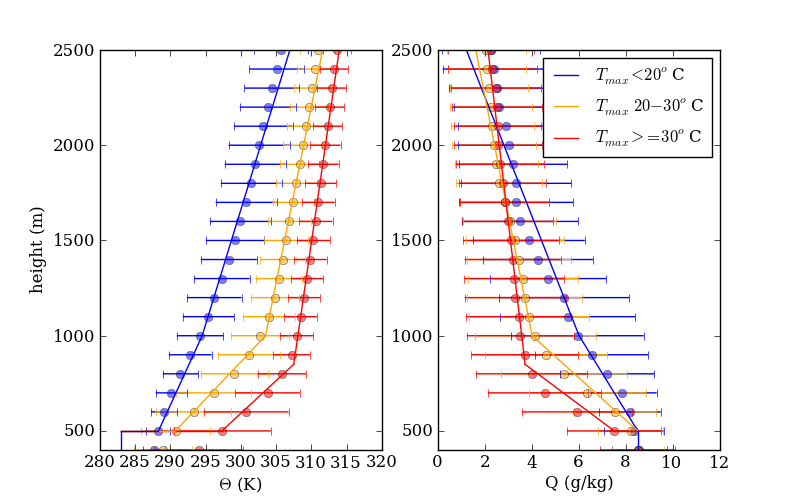
\includegraphics[width=1\textwidth]{ch2-BL/figures/fitted_lapserates_theta_Q_onefig.png}
\caption{}
\label{fig:BL_LapseRates}
\end{figure}

The range of soil moisture, free troposphere, and tree species conditions tested are listed in Table \ref{table:BL_1Druns}.  

\begin{table}
\begin{tabular}{ l c }
\hline
 & Range of values tested \\ \hline
Jarvis $VPD$ and $\theta_{rel}$ parameters & Douglas fir, Pacific madrone (Table XXX)\\
Lapse rates $\Gamma_{\Theta}$ and $\Gamma_Q$ & 1 (blue in Figure \ref{fig:BL_LapseRates}), 2 (yellow), 3 (red)\\
Relative soil moisture $\theta_{rel}$ & 0.15, 0.2, 0.25, 0.3, 0.35, 0.4, 0.45, 0.5\\
\hline
\end{tabular}
\caption{Range of values tested using the one-dimensional boundary layer model.}
\label{table:BL_1Druns}
\end{table}

\subsection{Regional climate model}
In order to further test the impact of these two tree species on the atmospheric boundary layer, we use WRF-Noah [Skamarock \textit{et al.}, 2008], a three-dimensional, non-hydrostatic regional climate model (Weather Research and Forecasting, or WRF) with terrain-following vertical coordinates and a coupled land surface model (Noah).  In WRF, the conservation equations for momentum, mass, and energy are solved numerically to calculate the temporal evolution of atmospheric state variables, including air temperature, pressure, humidity, and wind velocity.  

\begin{table}
\begin{tabular}{l l}
\hline
Scheme & Setting \\ \hline
WRF version & 3.6 \\
Grid nesting & two-way \\
Lateral boundary conditions & NCEP Eta analysis \\
Soil levels & 4 \\
Land use and soil categories & USGS \\
Land surface model & Noah \\
Surface layer & MM5 Monin-Obukhov \\
Planetary Boundary Layer (PBL) & ACM2 \\
Microphysics & WSM 3-class simple ice \\
Longwave radiation & RRTM \\
Shortwave radiation & Dudhia \\
Cumulus & Kain-Fritsch (new Eta) \\
Turbulence closure & Horizontal Smagorinzky first order \\
Momentum advection & 5th order horizontal, 3rd order vertical \\
Scalar advection & Positive definite \\
Lateral boundary & 5 grid points \\
\hline
\end{tabular}
\caption{WRF parameterization options.  See Skamarock \textit{et al.} [2008] for description of schemes.}
\label{table:BL_paramschemes}
\end{table}

Subgrid processes, including radiation, planetary boundary layer (PBL) turbulence, cloud microphysics, and convection, are parametrized in WRF, and the parametrization schemes used here are listed in Table \ref{table:BL_paramschemes}.  The ACM2 PBL scheme was used because of its ability to represent both convective regimes (non-local transport) and shear-dominated regimes (local transport) [Pleim, 2007], and because of its good performance in other WRF studies [CITATIONS including Marjanovic].

\begin{table}
\begin{tabular}{ l c c c c c c c }
\hline
Domain & $\Delta x$ (km) & $\Delta y$ (km) & $nx$ & $ny$ & $nz$ & $\Delta t$ (s) & USGS data res \\ \hline
d01 & 8.1 & 8.1 & 96 & 99 & 45 & 45 & 2 min\\
d02 & 2.7 & 2.7 & 175 & 175 & 45 & 15 & 2 min\\
\hline
\end{tabular}
\caption{Model domains. d01 refers to the outer domain, and d02 refers to the inner domain.}
\label{table:BL_domains}
\end{table}

The tests are run with two nested domains centered on the northern Coast Range (Figure XX).  The domains are two-way nested, meaning that the outer domain (d01) provides the lateral boundary conditions for the inner domain (d02), and the inner domain states are fed back to the outer domain throughout the region coincident with the inner domain.  Two-way nesting improves model accuracy, particularly in regions of complex terrain [CITATIONS].  The domain resolutions and dimensions are listed in Table \ref{table:BL_domains}.  The lateral boundaries of the outer domain are forced with NCEP Eta 212 grid (40 km) operational analysis [NCEP, 1998] for the period of 2009-08-16 00:00 to 2009-08-30 00:00, with the first 32 hours discarded as model spin-up.  This time period is rain-free and sunny at the Angelo Reserve and represents the mid- to late-summer season when soil moisture is highly limited and incoming radiation is still strong (cf. Chapter XX Figure XX - rivendell met time series).

Observed topography and USGS vegetation and soil types are used, with the exception of the northern Coast Range region highlighted in Figure XX, where the vegetation and soil types are assigned to dummy types.  The VPD and soil moisture stomatal response parameters of this dummy type are modified according to the test case as described below.  Radiative properties, leaf area, and rooting depth of the dummy type are held constant among the test cases, using the ``Evergreen Needleleaf Forest'' values.

\begin{table}
\begin{tabular}{ l p{3cm} p{3cm} p{2cm} p{3cm} }
\hline
Vegetation type & $\theta_{ref}$ (m$^3$/m$^3$) & $\theta_{wilt}$ (m$^3$/m$^3$) & RS (s/m) & HS (kg/kg)\\ \hline
ENF & 0.329 (loam) & 0.066 (loam) & 125 & 47.35\\
Douglas fir & 0.156 & 0.075 & 125 & 47.35\\
EBF & 0.329 (loam) & 0.066 (loam) & 150 & 41.69\\
Pacific madrone 1 & 0.105 & 0.047 & 550 & 10.\\
Pacific madrone 2 & 0.105 & 0.047 & 300 & 20.\\
\hline
\end{tabular}
\caption{Parameters for Noah's Jarvis formulation of stomatal conductance, by vegetation type.  RS is the Noah minimum stomatal resistance parameter in the Jarvis formulation. HS is the Noah scaling factor for the specific humidity deficit in the Jarvis humidity stress function (Equation XX). ENF is the USGS Evergreen Needleleaf Forest land use type; EBF is the USGS Evergreen Broadleaf Forest land use type.}
\label{table:BL_NoahJarvisparams}
\end{table}

\begin{table}
\begin{tabular}{ l p{6cm} p{7cm} }
\hline
Run ID & VPD parameters (RS, HS) & Soil moisture parameters ($\theta_{ref}$, $\theta_{wilt}$)\\ \hline
vDF-sDF & Douglas fir (ENF) & Douglas fir\\
vEBF-sMD & EBF & Pacific madrone\\
vMD1-sMD & Pacific madrone 1 & Pacific madrone\\
vMD2-sMD & Pacific madrone 2 & Pacific madrone\\
\hline
\end{tabular}
\caption{Combinations of stomatal conductance Jarvis parameters used in the WRF tests.  Each pair of parameters is tested for a range of volumetric soil moisture values in the northern Coast Range test region: 0.08, 0.1, 0.12, and 0.14 m$^3$/m$^3$.}
\label{table:BL_WRFruns}
\end{table}

The Noah model uses a Jarvis formulation of stomatal conductance similar to that used in Chapter XX (Equation XX).  The XX parameter is the minimum stomatal resistance (equivalent to $1/g_s$), and XX is divided by empirical functions of environmental variables.  The soil moisture stress function is the piecewise-linear, threshold Feddes model [\textit{Feddes et al.}, 1978; \textit{Chen et al.}, 2008].  The parameters for the sigmoid model from Chapter XX (Equation XX, Table XX) thus must be translated to the Feddes parameters (reference or stress point, $\theta_{ref}$, and wilting point, $\theta_{wilt}$).  For each species, we fit a line to $f_{\theta}$ between $f_{\theta}=0.05$ and $f_{\theta}=0.95$ and extrapolate the line to 0 to estimate $\theta_{wilt}$ and to 1 to estimate $\theta_{ref}$ (Figure \ref{fig:BL_FeddesParams}, Table \ref{table:BL_NoahJarvisparams}).


Soil moisture in the Coast Range test region is reset each day at midnight local time, so that the soil moisture deviates only minimally from its stated value (e.g. Figure XX shows one of the wettest cases, XXXX, with a daily decline of XX m$^3$/m$^3$ or less).

The empirical function representing humidity stress is similar to the \textbf{Lohammar} function used in Chapter XX (Equation XX):

\textbf{WRF Q EQUATION}

The $1/rsmin * f(VPD)$ using USGS parameters for Evergreen Needleleaf Forest (ENF, COLOR) and Evergreen Broadleaf Forest (EBF, COLOR) are shown in Figure XX (top panel).  For comparison, the $g_{s, max}/\alpha * f(VPD)$ calculated using sap-flow-derived species averaged parameters for Douglas fir and Pacific madrone (Chapter XX, Table XX) are also shown in Figure XX (bottom panel).  The ENF and Douglas fir $g_s$ respond very similarly to humidity stress, so the existing ENF parameters are used to represent the Douglas fir.  The model EBF $g_s$ is much higher than is the Pacific madrone $g_s$ at low $VPD$ (relative to ENF or Douglas fir, respectively).  As such, we run tests with the EBF VPD parameters representing Pacific madrone (parameters listed in Table \ref{table:BL_NoahJarvisparams}; runs TEST NAMES, Table XX), but we also test two additional rsmin-hs parameter pairs that more closely approximate the shape of the sap-flow-derived curve for Pacific madrone (COLORS lines in Figure XX; parameters listed in Table \ref{table:BL_NoahJarvisparams}; runs TEST NAMES, Table XX).

\begin{figure}[here]
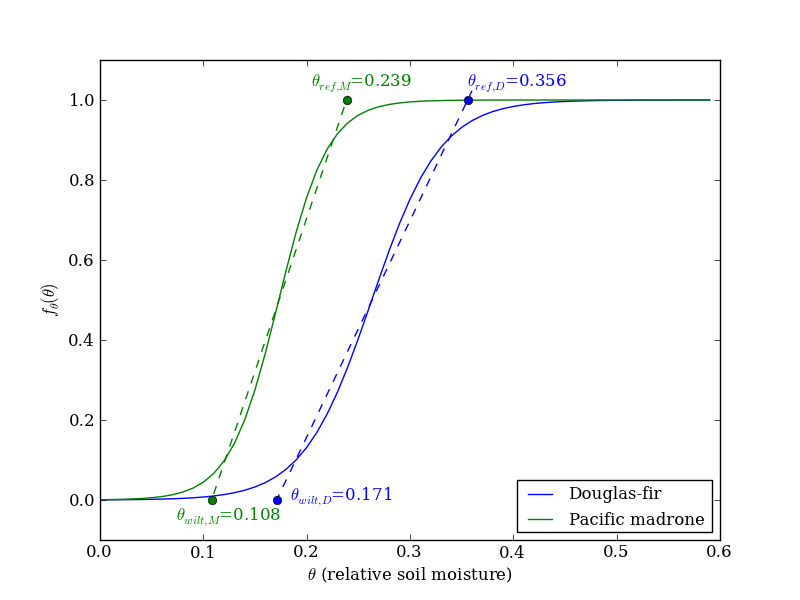
\includegraphics[width=1\textwidth]{ch2-BL/figures/theta_params.png}
\caption{}
\label{fig:BL_FeddesParams}
\end{figure}


WRF-Noah is run using the permutations of stomatal response parameters listed in Table \ref{table:BL_NoahJarvisparams}, with a range of soil moisture values (0.08, 0.1, 0.12, 0.14).  These values are equivalent to relative soil moistures of XXXX, given that the saturation moisture content of the loam soil type used in the model is 0.439 m$^3$/m$^3$.  These relative soil moisture values span the range of values observed in August at the Angelo Coast Range Reserve (Chapter XX, Figure XX).

\section{Results}

\subsection{1-D model}

\begin{figure}[here]
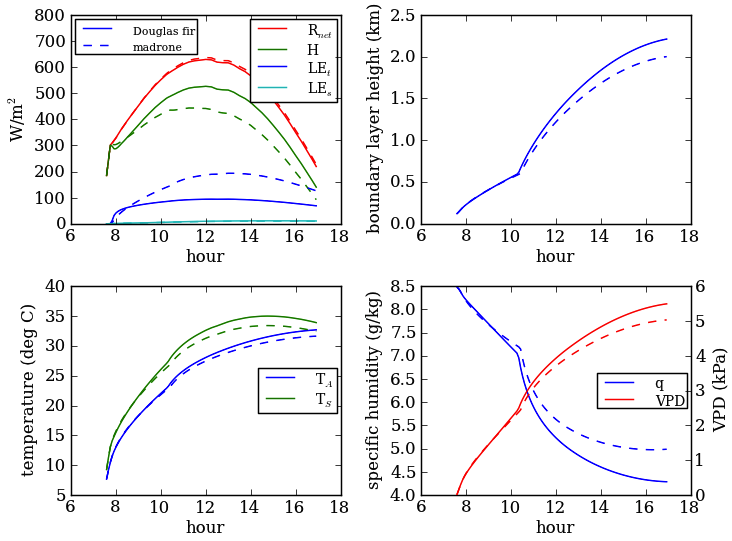
\includegraphics[width=0.9\textwidth]{ch2-BL/figures/testall_Aug15_soilm0pt25_ra10_lapseT2_cropped.png}
\caption{Diurnal cycle simulated by 1-D model for $\theta_{rel}=0.25$ and lapse rate \#2.  Solid lines: Douglas fir case; dashed lines: Pacific madrone case.  Top left: surface energy flux terms ($R_{net}$ is net radiation, $H$ is sensible heat, $LE_t$ is latent heat due to transpiration, and $LE_s$ is latent heat due to soil evaporation.)  Top right: boundary layer height.  Bottom left: surface temperature ($T_S$) and mixed layer air temperature ($T_A$) adjusted to 400 m ASL (ground level in ACRR).  Bottom right: mixed layer specific humidity ($q$) and $VPD$.}
\label{fig:BL_1Ddiurnal}
\end{figure}

The 1-D model simulates a reasonable diurnal cycle for mid-August, but with temperatures several degrees higher than observations at the ACRR, which may result from using tropospheric soundings from Oakland.  Figure \ref{fig:BL_1Ddiurnal} shows a typical diurnal cycle for a moderate lapse rate (\#2) and relative soil moisture $\theta_{rel} = 0.25$.  The Pacific madrone forest has higher transpiration than the Douglas fir forest, because Pacific madrone stomatal conductance is higher at this value of $\theta_{rel}$ (c.f. Figure \ref{fig:BL_FeddesParams}); both cases have very little soil evaporation at this value of $\theta_{rel}$.  As a result, the Pacific madrone case has lower sensible heat ($H$) than the Douglas fir case, leading to a shallower, cooler, and moister boundary layer over the Pacific madrone forest.

\begin{figure}[here]
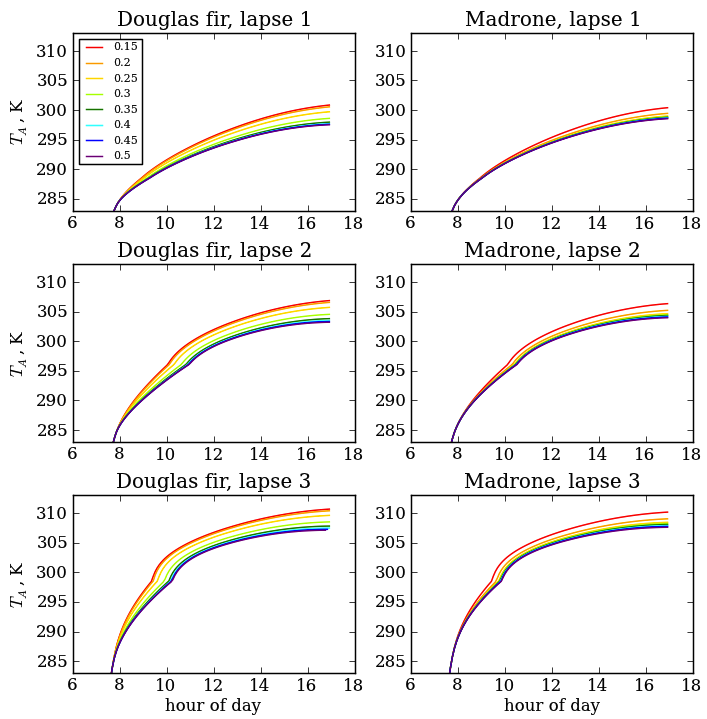
\includegraphics[width=0.9\textwidth]{ch2-BL/figures/testall_compare_sm_lapse_Ta_cropped.png}
\caption{Diurnal cycle of air temperature at 400 m ASL (ground level in ACRR), simulated by the 1-D model, for a range of $\theta_{rel}$ (colors) and free troposphere conditions.  Left column: Douglas fir case; right column: Pacific madrone case.  Top row: lapse rate 1 (coolest free troposphere conditions); middle row: lapse rate 2 (moderate free troposphere conditions); bottom row: lapse rate 3 (warmest free troposphere conditions).}
\label{fig:BL_1DdiurnalTa}
\end{figure}

\begin{figure}[here]
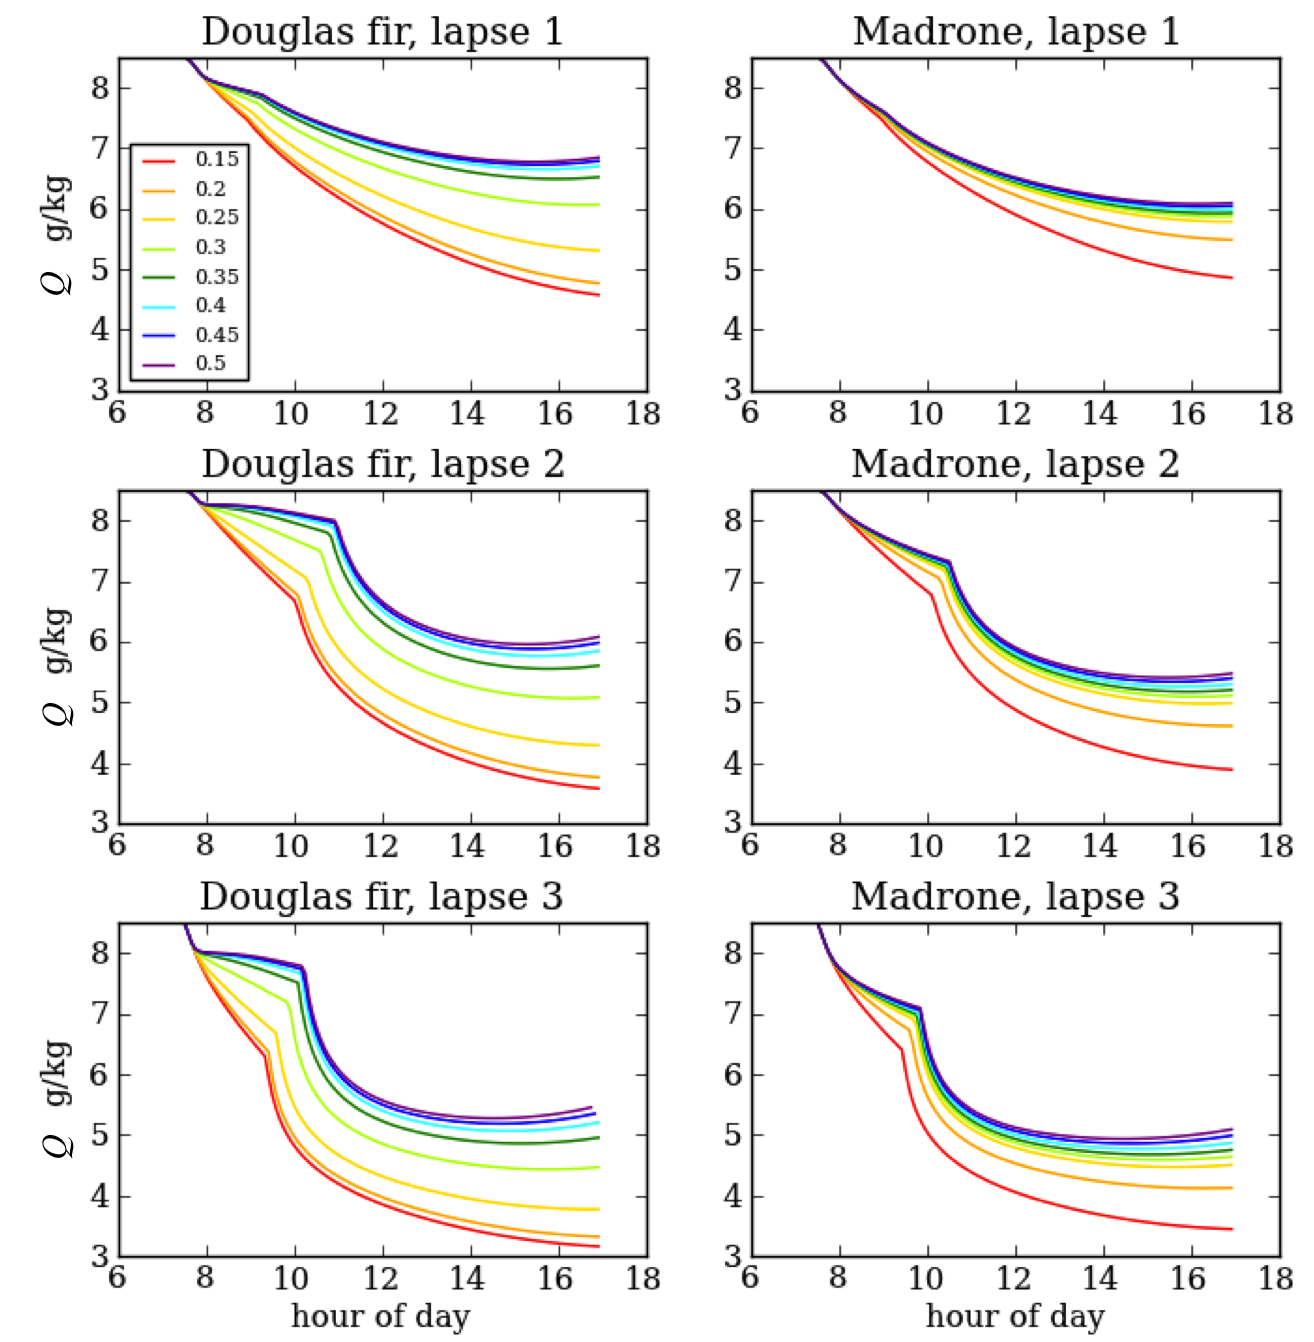
\includegraphics[width=0.9\textwidth]{ch2-BL/figures/testall_compare_sm_lapse_Q_cropped2.png}
\caption{Diurnal cycle of boundary layer specific humidity, simulated by the 1-D model, for a range of $\theta_{rel}$ (colors) and free troposphere conditions.  Left column: Douglas fir case; right column: Pacific madrone case.  Top row: lapse rate 1 (most moist free troposphere conditions); middle row: lapse rate 2 (moderate free troposphere conditions); bottom row: lapse rate 3 (driest free troposphere conditions).}
\label{fig:BL_1DdiurnalQ}
\end{figure}

%\clearpage

The boundary layer is warmer and drier when the free troposphere is warmer and drier (Figures \ref{fig:BL_1DdiurnalTa} and \ref{fig:BL_1DdiurnalQ}; increasing $T_a$ and decreasing $Q$ from lapse rate 1 to 2 to 3).  Additionally, the shape of the diurnal cycle differs among the free troposphere cases, with most rapid morning increase in $T_a$ in the hottest case (lapse rate 3), due to entrainment of high-$\Theta$ air in the steep low-level inversion.  The drier free troposphere conditions in lapse rate 3 also lead to lower $Q$, but with a slower morning decline of $Q$ because of relatively slow boundary layer growth through the steep inversion.

\begin{figure}[here]
\begin{subfigure}{0.5\textwidth}
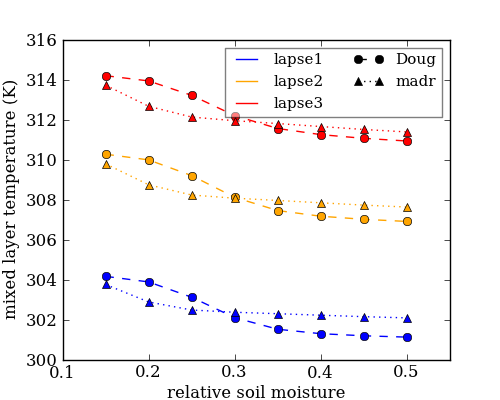
\includegraphics[width=\textwidth]{ch2-BL/figures/all_afternoon_T.png}
\caption{}
\end{subfigure}
\begin{subfigure}{0.5\textwidth}
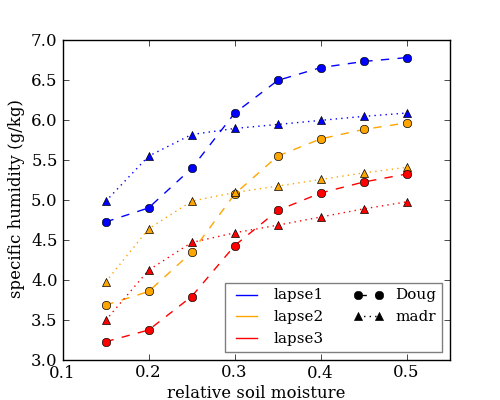
\includegraphics[width=\textwidth]{ch2-BL/figures/all_afternoon_Q.png}
\caption{}
\end{subfigure}
\caption{Conditions at 3:45 pm in the 1-D model, as a function of soil moisture, for the three free troposphere lapse rates (colors).  (a) Air temperature at 400 m ASL (ground level in ACRR), and (b) specific humidity.  Dashed lines with circles: Douglas fir case.  Dotted lines with triangles: Pacific madrone case.}
\label{fig:BL_345changes}
\end{figure}

%\clearpage

For both the Pacific madrone forest and the Douglas fir forest, drier soil (decreasing $\theta_{rel}$) leads to a warmer and drier boundary layer (increasing $T_a$ and decreasing $Q$).  However, in the Douglas fir case, the increase in $T_a$ and decrease in $Q$ begin when the soil is wetter ($\theta_{rel} \le 0.3$; Figures \ref{fig:BL_1DdiurnalTa} and \ref{fig:BL_1DdiurnalQ}, left columns), while in the Pacific madrone case, the increase in $T_a$ and decrease in $Q$ begin only when soil is drier ($\theta_{rel} \le 0.2$; Figures \ref{fig:BL_1DdiurnalTa} and \ref{fig:BL_1DdiurnalQ}, right columns).  

The differences between the species cases are largest in the afternoon; Figure \ref{fig:BL_345changes} shows $T_a$ and $Q$ at 3:45 pm for the Douglas fir and Pacific madrone cases, as a function of $\theta_{rel}$ and free troposphere conditions.  The differences between the Douglas fir and Pacific madrone cases for both $T_a$ and $Q$ are largest at $\theta_{rel}$ values around 0.2, with the Douglas fir case hotter by 1-1.5 $^\circ$C and drier by $\sim$0.7 g/kg.  A $\theta_{rel}$ value of 0.2-0.25 is typical for the mid- to late-dry-season at the ACRR (Figure \ref{fig:sapflow_met}). Interestingly, at $\theta_{rel}$ values higher than about 0.35, the Douglas fir case is actually cooler and moister; such $\theta_{rel}$ values are typical for the late spring and early summer at the ACRR (Figure \ref{fig:sapflow_met}).

\begin{figure}[here]
\begin{subfigure}{0.5\textwidth}
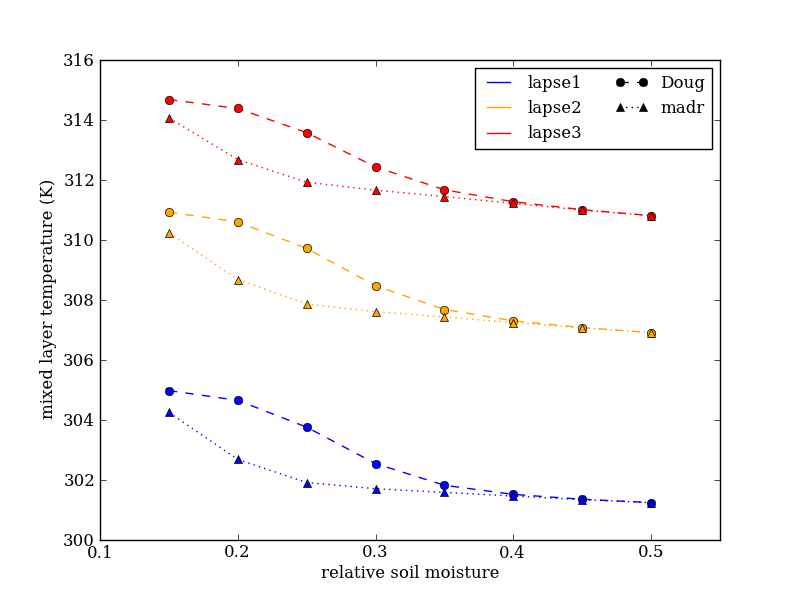
\includegraphics[width=\textwidth]{ch2-BL/figures/theta_afternoon_T.png}
\caption{}
\end{subfigure}
\begin{subfigure}{0.5\textwidth}
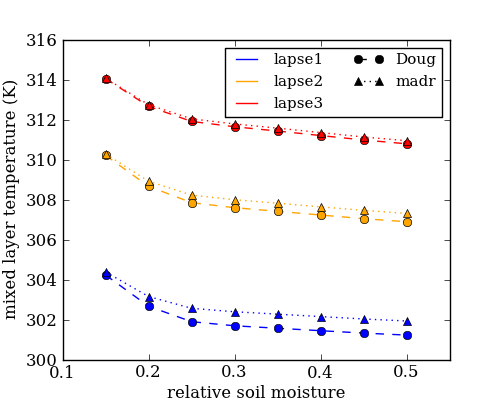
\includegraphics[width=\textwidth]{ch2-BL/figures/VPD_afternoon_T.png}
\caption{}
\end{subfigure}
\caption{Air temperature at 400 m ASL (ground level in ACRR) at 3:45 pm in the 1-D model, as a function of soil moisture, for the three free troposphere lapse rates (colors).  (a) holding $VPD$ parameters constant at Douglas fir values and varying $\theta$ parameters by species, and (b) holding $\theta$ parameters constant at Pacific madrone values and varying $VPD$ parameters by species.}
\label{fig:BL_testVPDtheta}
\end{figure}

The temperature and humidity differences at $\theta_{rel} \le 0.3$ are due largely to Douglas firs' greater stomatal closure with dry soil.  Model tests setting the $VPD$ parameters ($D_o$ and $g_{c,max}$) to the Douglas fir values (Table \ref{tbl:sapflow_mcmc}) and varying the $\theta$ parameters ($\theta_0$ and $\beta$) by species give a Douglas fir - Pacific madrone temperature difference of 1.5-2$^\circ$C at $\theta_{rel} = 0.2$ (Figure \ref{fig:BL_testVPDtheta}(a)), while tests setting the $\theta$ parameters to the Pacific madrone values and varying the $VPD$ parameters by species give a temperature difference of \textless 0.5$^\circ$C at $\theta_{rel} = 0.2$ (Figure \ref{fig:BL_testVPDtheta}(b)).  Thus, in dry soil, the Douglas fir $VPD$ response does little to moderate the temperature differences caused by Douglas fir stomatal closure at low $\theta_{rel}$.  However, in wet soils ($\theta_{rel}$ \textless $0.3$), and particularly in cool free troposphere conditions, the greater Douglas fir stomatal conductance at low $VPD$ cools the boundary layer (Figure \ref{fig:BL_testVPDtheta}(b)), while soil moisture plays little role (Figure \ref{fig:BL_testVPDtheta}(a)).

%- fraction of moisture from land surface vs. from free troposphere, for different soil moisture / lapse rate / species conditions

\subsection{Regional climate model}

\begin{figure}[here]
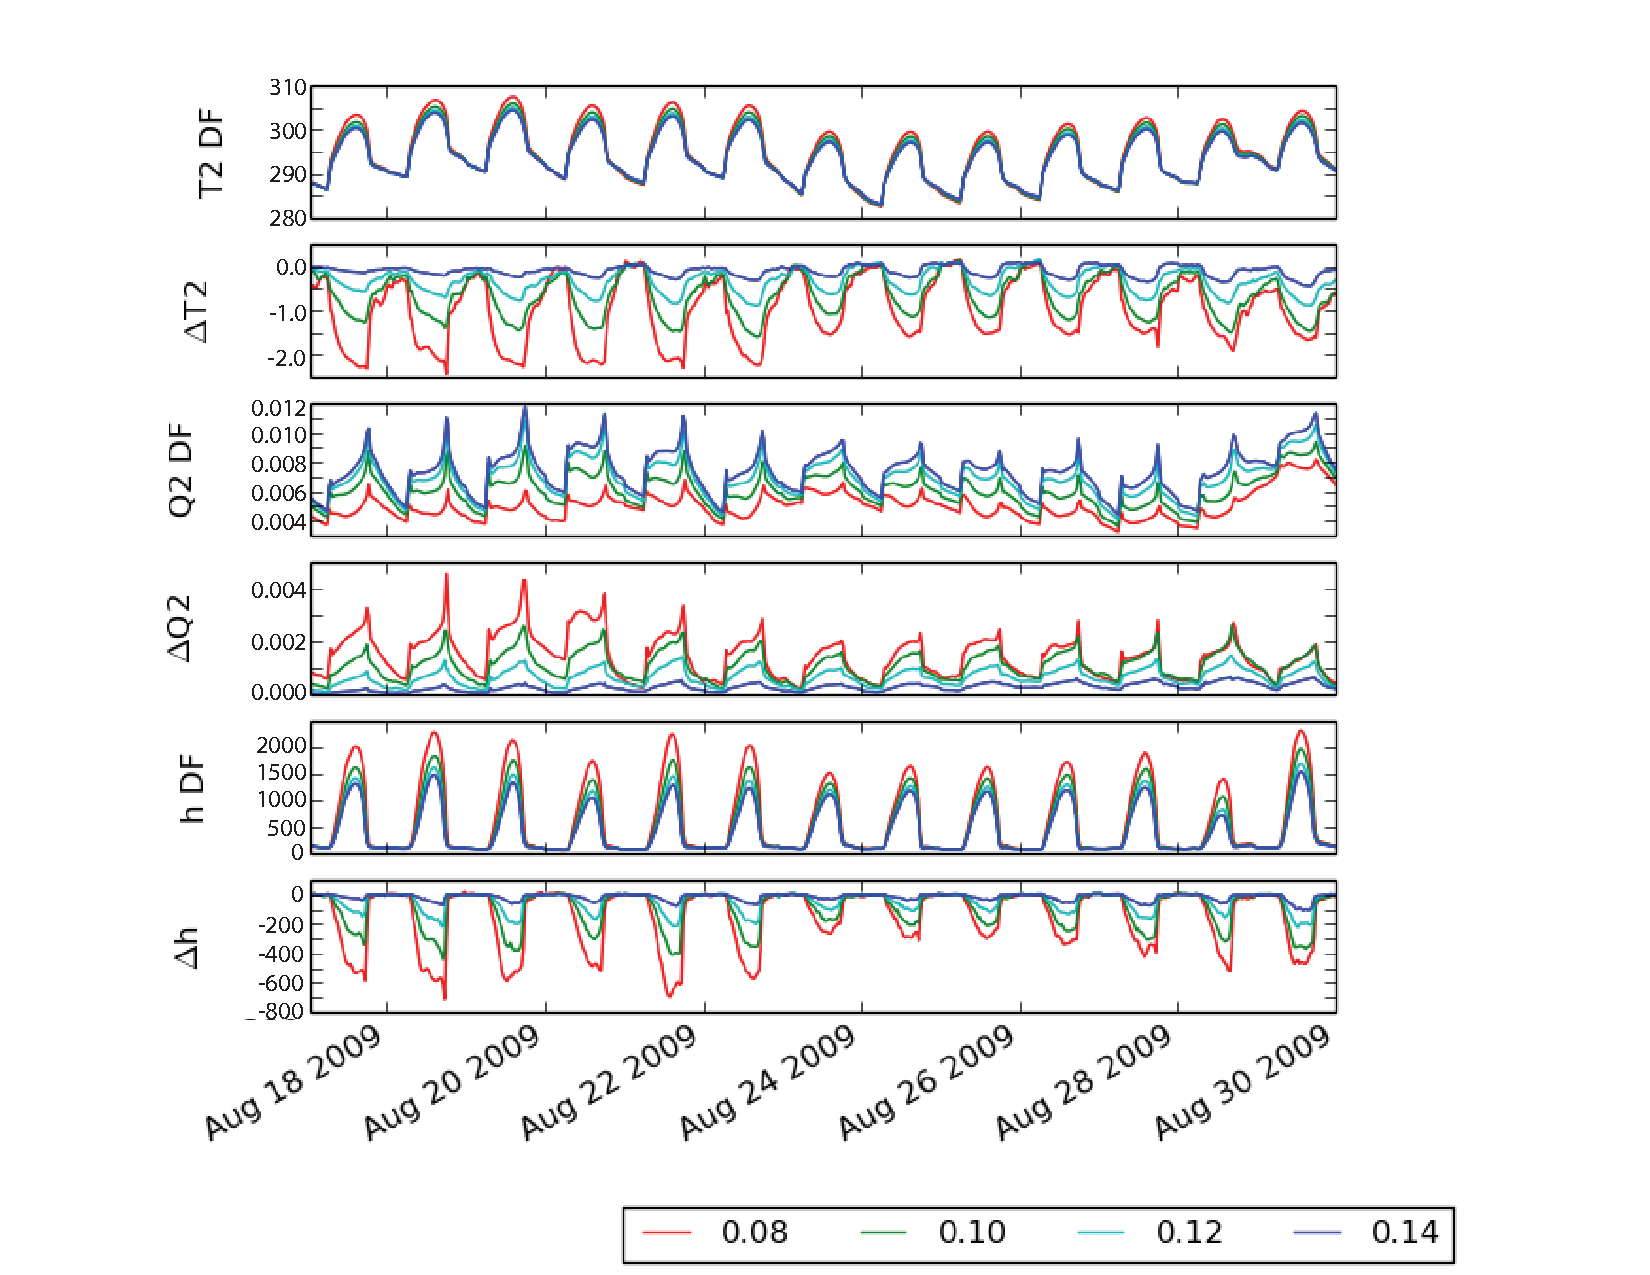
\includegraphics[width=\textwidth]{ch2-BL/figures/T_Q_h_d02.pdf}
\caption{Time series of near-surface conditions in the WRF tests, averaged over the test region, for a range of $\theta_{vol}$ values (colors).  Top panel: air temperature (K) at 2 m above ground level for the all-Douglas-fir case.  Second panel: difference in 2 m air temperature between the all-Pacific-madrone case and the all-Douglas-fir case.  Third panel: specific humidity ($q$, kg/kg) at 2 m above ground, for the all-Douglas-fir case.  Fourth panel: difference in 2 m $q$ between the all-Pacific-madrone case and the all-Douglas-fir case.  Fifth panel: boundary layer height in the all-Douglas-fir case.  Sixth panel: difference in boundary layer height between the all-Pacific-madrone case and the all-Douglas-fir case.}
\label{fig:BL_WRFtseries}
\end{figure}

Figure \ref{fig:BL_WRFtseries} shows the time series of atmospheric conditions averaged over the test region in the Douglas fir case (panels 1, 3, and 5) and the difference between the Pacific madrone and Douglas fir case (panels 2, 4, and 6).  In the Douglas fir case, drier soils lead to a hotter (panel 1 of Figure \ref{fig:BL_WRFtseries}), drier (panel 3), and deeper (panel 5) boundary layer than do wet soils.  For soil moisture $\le$ 0.12 m$^3$/m$^3$ ($\theta_{rel} \le 0.27$), the boundary layer over the madrone forest is cooler (panel 2), moister (panel 4), and shallower (panel 6) than that over the Douglas fir forest; the differences are negligible for soil moisture of 0.14 m$^3$/m$^3$ ($\theta_{rel} = 0.32$).  The differences between the species cases increase with drier soil: the greatest differences occur when soil moisture is 0.08 m$^3$/m$^3$, with 2 m air temperature in the madrone case cooler by 1.5-2.5$^\circ$C, 2 m humidity greater by 1-3 g/kg, and boundary layer depth shallower by 200-500 m, averaged over the test region.

\begin{figure}[here]
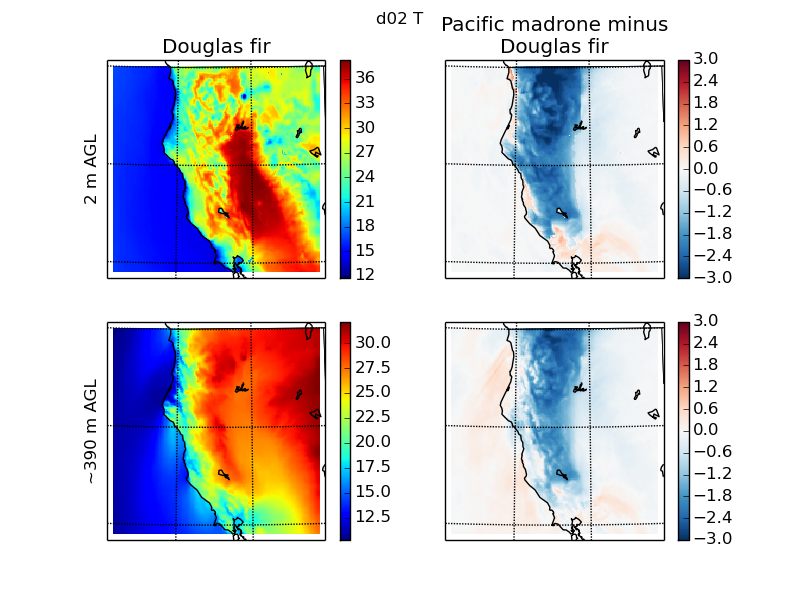
\includegraphics[width=1\textwidth]{ch2-BL/figures/T_d02_s0pt08.png}
\caption{Left column: temperature ($^\circ$C) in domain d02 for the Douglas fir case.  Right column: temperature difference between the Pacific madrone case and the Douglas fir case.  Top row: 2 m above ground level (AGL).  Bottom row: model level at $\sim$390 m AGL (380-395 m for the test region).}
\label{fig:BL_WRFmapT}
\end{figure}

\begin{figure}[here]
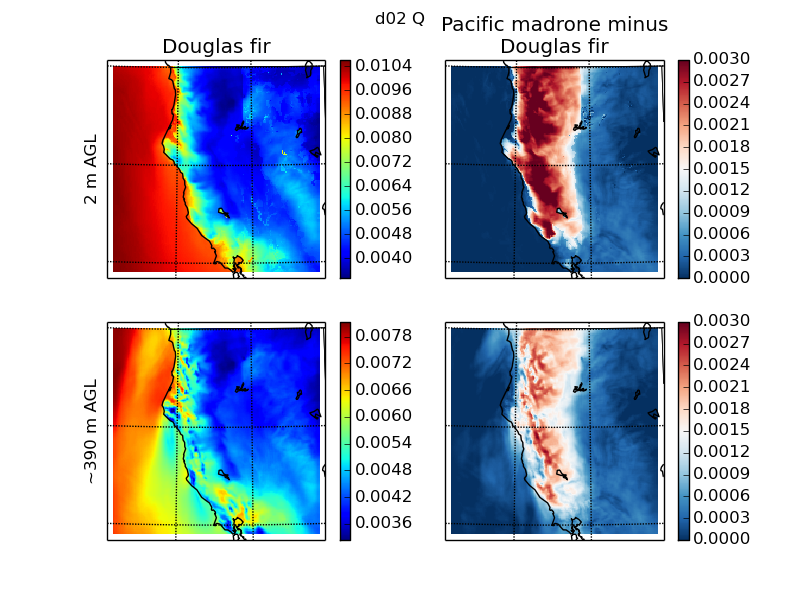
\includegraphics[width=1\textwidth]{ch2-BL/figures/Q_d02_s0pt08.png}
\caption{Left column: specific humidity (kg/kg) in domain d02 for the Douglas fir case.  Right column: specific humidity difference between the Pacific madrone case and the Douglas fir case.  Top row: 2 m AGL.  Bottom row: model level at $\sim$390 m AGL (380-395 m for the test region).}
\label{fig:BL_WRFmapQ}
\end{figure}

\begin{figure}[here]
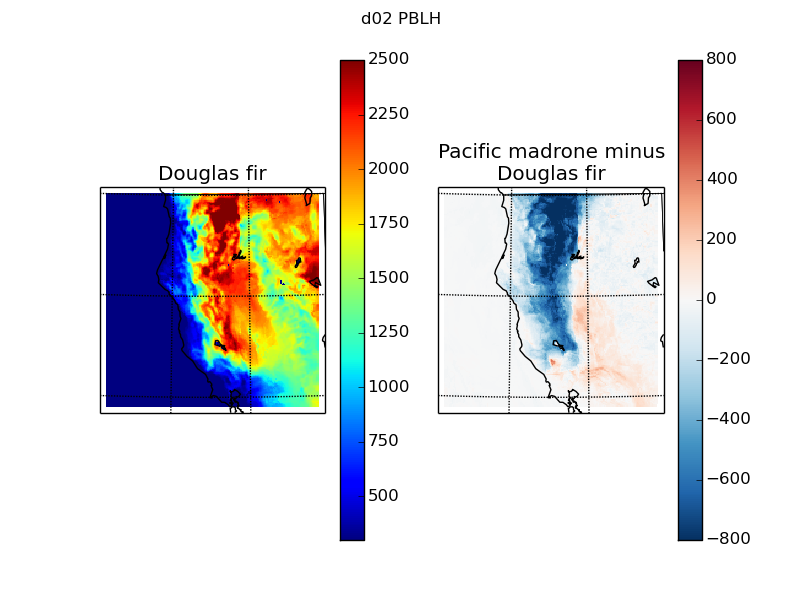
\includegraphics[width=1\textwidth]{ch2-BL/figures/PBLH_d02_s0pt08.png}
\caption{Left column: boundary layer height (m) in domain d02 for the Douglas fir case.  Right column: boundary layer height difference (m) between the Pacific madrone case and the Douglas fir case.}
\label{fig:BL_WRFmapPBLH}
\end{figure}

The differences in temperature and humidity persist from 2 m AGL (Figures \ref{fig:BL_WRFmapT} and \ref{fig:BL_WRFmapQ}, top rows) through to the mixed layer at $\sim$390 m AGL (Figures \ref{fig:BL_WRFmapT} and \ref{fig:BL_WRFmapQ}, bottom rows). The species differences are smaller at 390 m AGL than at 2 m AGL: the madrone case is cooler than the Douglas fir case by up to $\sim$2.5$^\circ$C at 2 m AGL and by up to $\sim$1.5$^\circ$C at 390 m AGL; humidity in the madrone case is greater than in the Douglas fir case by 2-3 g/kg at 2 m AGL and by 1.5-2.5 g/kg at 390 m AGL.

The changes in 390 m AGL temperature and humidity and in boundary layer depth are greatest inland, where the convective boundary layer is fully developed.  The boundary layer in the control Douglas fir case is shallow near the coast but deepens inland (Figure \ref{fig:BL_WRFmapPBLH}, left panel), as expected from previous analytical and numerical studies [\cite{garratt1990internal}].  Because the boundary layer is shallow in this zone, the differences in surface energy balance between the species cases may not be fully communicated to an altitude of 390 m AGL.  The deeper boundary layer inland means that the air at 390 m AGL is part of the mixed layer that communicates rapidly with the surface; thus, the changes in temperature and humidity in the madrone case affect the air at 390 m AGL over inland but not coastal regions.




\section{Discussion and Conclusions}

Large-scale conversion of the northern California Coast Range forest from all-Douglas-fir to all-Pacific-madrone cools and moistens the summertime boundary layer when relative soil moisture is less than 0.3, conditions typical of late summer at the ACRR (Figure \ref{fig:sapflow_met}).   Two atmospheric models, one simple and one complex, simulate a cooling of $\sim$1.5$^\circ$C in the mixed layer ($\sim$2.5$^\circ$C near the surface) and a moistening of 1 g/kg in the mixed layer (2-3 g/kg near the surface).  With 100\% Pacific madrone coverage compared with 100\% Douglas fir coverage, Pacific madrone cools and moistens the boundary layer when soils are dry because madrone stomatal conductance and thus transpiration remains higher at low soil moisture.  The greater transpiration consumes a larger fraction of net radiation in latent heat and reduces the sensible heat flux; because sensible heat is reduced, there is less direct heating of the boundary layer from the surface, and there is less entrainment of the hotter, drier free tropospheric air above the boundary layer.

The simple model and the complex model estimate similar magnitudes of temperature and humidity differences between the Douglas fir and Pacific madrone cases; the similarity of the results confirms the role of evapotranspiration in the near-surface atmosphere in the northern California Coast Range, especially in the dry season.  The 1-D boundary layer model does not include the effects of advection or subsidence and thus overestimates boundary layer height and temperature at the ACRR field site; however, the differences in temperature and humidity between the Douglas fir and Pacific madrone cases simulated by the simple model agree with the differences simulated by the complex model.  Even accounting for the effects of advection, complex topography, and subsidence in WRF, the hotter and drier conditions of the Douglas fir case relative to the Pacific madrone case are a robust result.

The differences in late summer temperature and humidity are due largely to the differences in stomatal response to soil water deficit (Figure \ref{fig:BL_testVPDtheta}).  Importantly, WRF does not represent vegetation-type differences in stomatal response to soil moisture; rather, the $\theta_{ref}$ and $\theta_{wilt}$ parameters depend only on soil type in WRF.  This inability to represent vegetation differences in water stress points prevents WRF from accurately representing the variation in land surface response to drought.  Adding vegetation-type-specific $\theta_{ref}$ and $\theta_{wilt}$ parameters to the WRF Noah land surface model would improve WRF's ability to simulate ecosystem-atmosphere interactions.

While we incorporate sap-flow-derived parameters for stomatal response to soil moisture in both models, in the WRF tests we do not use sap-flow-derived parameters for the $VPD$ response.  In order to incorporate sap-flow-derived $VPD$ parameters into WRF in future work, measurements of the sapwood area to leaf area ratio are necessary (for converting $g_{s,max}$, representing conductance on a per-sapwood-area basis, to $1/RS$, representing stomatal conductance on a per-leaf-area basis).  The sap-flow-based $VPD$ parameters should also be re-estimated using $\Delta q$ instead of $VPD$, in accord with the WRF humidity stress function (Equation \ref{eqn:BL_WRFq}).  Nevertheless, the effect of differences in $VPD$ parameters is small when $VPD$ is high and soil is dry, as is the case in mid- to late-summer (Figure \ref{fig:BL_testVPDtheta}).  The effect of differences in $VPD$ parameters may be larger when soil is wet and $VPD$ is low to moderate, as in winter and spring; simulations of those conditions would require more accurate estimation of species-specific $VPD$ parameters.

Using sap flow measurements to parameterize a regional climate model requires a significant scale jump, from the scale of whole trees and a single hillslope, to the scale of 2.7 km grid boxes and a 500 km x 500 km domain.  Such scale jumps are inherent in the measurement of evapotranspiration; however, further sap flow measurements of these species on slopes with different aspects, elevations, and species mixes are needed in order better to quantify the variability in stomatal response parameters and covariation with other environmental conditions.

The regional cases tested here are extreme scenarios involving the total conversion of the forest from one species (Douglas fir) to the other (Pacific madrone).  However, this may not be wholly unrealistic: Pacific madrones were likely more abundant in the past, due to regular controlled burning by indigenous people [\cite{johnsonACRR}].  It is possible that longer and more severe droughts in a warmer future climate could cause a shift from Douglas fir to Pacific madrone, if fires become more frequent and if Douglas firs are less tolerant of drought.  Moreover, forest management stakeholders are actively discussing controlling the encroachment of Douglas fir in this region [William Dietrich, personal communication]. This study demonstrates that such regional-scale species shifts could have regional-scale impacts on air temperature and humidity in the dry season.

In this study, we integrate tree-scale field observations with physical atmospheric models to test regional atmospheric feedbacks of species-specific stomatal behavior.  We demonstrate the sensitivity of the boundary layer to stomatal dynamics and show that a regional-scale change in dominant evergreen tree species can change summertime afternoon near-surface temperatures by $\sim$2$^\circ$C.  This result underscores the importance of understanding species- and vegetation-type-differences in stomatal response to soil moisture and $VPD$.

%%\documentclass[12pt]{amsart}
%\usepackage{geometry} % see geometry.pdf on how to lay out the page. There's lots.
%\usepackage{datetime}
%\usepackage{setspace}
%\usepackage{graphicx}
%\usepackage{caption}
%\usepackage{subcaption}
%\doublespacing
%\geometry{a4paper} % or letter or a5paper or ... etc
%\DeclareMathOperator*{\argmin}{argmin}

% See the ``Article customise'' template for come common customisations

%\title{Wind chapter}
%\author{Percy Link}
%\date{\currenttime  \today}

\chapter{Wind Chapter}
\label{c.wind}

Abstract.


%%% BEGIN DOCUMENT
%\begin{document}

%\maketitle


%\documentclass[12pt]{amsart}
%\usepackage{geometry} % see geometry.pdf on how to lay out the page. There's lots.
%\usepackage{datetime}
%\geometry{a4paper} % or letter or a5paper or ... etc
%% \geometry{landscape} % rotated page geometry
%
%% See the ``Article customise'' template for come common customisations
%
%\title{Wind chapter}
%\author{Percy Link}
%\date{\currenttime \ \today} % delete this line to display the current date
%
%%%% BEGIN DOCUMENT
%\begin{document}
%
%\maketitle

\section{Introduction}

In this chapter, we investigate the effect of changes in land surface heat fluxes, mediated by modifications in soil moisture, on near-surface winds in California.  Accurate understanding and simulation of near-surface winds is necessary for a range of applications, including water vapor and pollutant transport studies, weather forecasting, aviation, and wind energy forecasting.  Here, we focus on wind forecasting for wind energy applications and on winds at a specific wind farm, the Solano Wind Project in the Sacramento-San Joaquin River Delta region of California.  A regional atmospheric model is used to test the sensitivity of Solano winds to different regions' soil moisture and to quantify the magnitude of the effect at different times of day across a range of soil moisture changes.  We demonstrate that accurate soil moisture information can improve wind forecasts.  This study serves as a prototype for characterizing the importance of soil moisture information for wind forecasts at other wind farms.

Accurate wind forecasts can reduce the cost of integrating wind energy into the electric grid on a large scale.  In order to reduce CO$_2$ emissions to the degree necessary to avert dangerous climate change [\cite{stocker2013ipcc}], electric utilities will need to transition to non-fossil-fuel energy sources, including a large fraction of wind energy [\cite{jacobson2011providing}].  However, although wind energy has large peak generation potential, it is intermittent, and the instantaneous mismatch between wind generation and electric demand must be met with other generation.  In most utilities, allocations of conventional electric generation (coal, natural gas, hydroelectric, and nuclear) are made one day in advance, based on forecasted net demand (demand minus wind and solar supply).  At shorter lead times (hour-ahead to real-time), imbalances between the day-ahead allocations of conventional generation and the actual net demand must be met with, in the case of a shortfall, more expensive quick-startup generation, or in the case of excess generation, wasted energy resources.  These imbalance costs add significantly to the cost of wind energy (around 10\% of a wind generator's income in a liberalized market [\cite{fabbri2005assessment}]).  Improved accuracy of wind forecasts could reduce imbalance costs, making integration of wind into the electric grid more economically feasible: wind and solar forecasting could reduce energy costs by \$0.01 to \$0.02 per kWh at 30\% wind and solar penetration [\cite{energy2010western}], or 8-15\% of the average US cost of electricity (\$0.13/kWh in July 2014 [\cite{eia2014}]).

%; and at high wind penetration, \$68 million to \$160 million could be saved annually in California using current state of the art forecasting, with an opportunity to save \$19 million to \$38 million more with forecast accuracy improvements [Porter and Rogers, 2010].

The major wind forecasting companies in North America and Europe use numerical weather prediction (NWP) models to make their day-ahead forecasts, often in combination with statistical post-processing [\cite{porter2010status}; \cite{foley2012current}; \cite{monteiro2009wind}].  NWP models simulate atmospheric wind speed, temperature, pressure, and humidity (among other variables) by solving the equations for conservation of momentum, mass, and energy, discretized in three spatial dimensions and in time.  NWP models require bottom boundary fluxes of energy, moisture, and momentum, but little attention has been paid to these bottom boundary fluxes in the wind energy literature (with the notable exceptions of \cite{marjanovic2014} and \cite{wharton2011review}, discussed below).  Wind energy forecast research has concentrated instead on sensitivity to NWP physical parameterizations, especially planetary boundary layer (PBL) schemes [\cite{draxl2014evaluating}; \cite{marjanovic2014}], and to grid resolution [\cite{marjanovic2014}, \cite{carvalho2012sensitivity}].  There have also been extensive efforts to enhance NWP wind energy forecasts by running model ensembles [\cite{deppe2013wrf}; \cite{pinson2009ensemble}] and by applying various model output statistics (MOS) algorithms [\cite{bedard2013development}; \cite{ranaboldo2013implementation}; \cite{ellis2014predicting}; \cite{ortiz2011short}; \cite{kusiak2009wind}].

%The prediction of ramps (rapid increases or decreases in wind power) remains a challenge [Carcangiu \textit{et al.}, 2014; Ellis \textit{et al.}, 2014; Wharton \textit{et al.}, 2011].

%Regional NWP models require boundary condition information at the lateral boundaries of the grid, as well as bottom boundary fluxes of energy, moisture, and momentum.  If the bottom boundary is land, these fluxes are usually calculated with a land surface model.  

%Wind energy forecasts are sensitive to NWP model resolution and physical parameterizations, especially planetary boundary layer (PBL) schemes [Draxl \textit{et al.}, 2014; Marjanovic \textit{et al.}, 2014]; the optimal PBL scheme depends in part on atmospheric stability conditions [Draxl \textit{et al.}, 2014; Marjanovic \textit{et al.}, 2014], and the optimal grid resolution depends largely on terrain complexity, with more complex terrain requiring higher resolution [Marjanovic \textit{et al.}, 2014, Carvalho \textit{et al.}, 2012].  Ensembles of NWP runs have been used to characterize a forecast probability distribution [Deppe \textit{et al.}, 2013; Pinson and Madsen, 2009].  Various model output statistics (MOS) algorithms incorporating historical observations have been shown to improve NWP forecasts in post-processing; in particular, machine learning algorithms such as directional multipoint linear regression [B\'edard \textit{et al.}, 2013], multiple linear regression [Ranaboldo \textit{et al.}, 2013], random forests, generalized linear models, gradient boosting, and support vector machines [Ellis \textit{et al.}, 2014; Ortiz-Garc\'ia \textit{et al.}, 2011], and neural networks [Kusiak \textit{et al.}, 2009] have shown promise.  The prediction of ramps (rapid increases or decreases in wind power) remains a challenge [Carcangiu \textit{et al.}, 2014; Ellis \textit{et al.}, 2014; Wharton \textit{et al.}, 2011].

The influence of soil moisture and land surface heating on wind prediction has received little attention in the wind energy forecasting literature, even though fluxes of energy at the land surface are known to influence regional circulations.  Soil moisture heterogeneity, and the resulting contrasts in sensible heat flux, can drive mesoscale circulations on land with wind speeds of several m/s [\cite{chen1994impact}; \cite{avissar1998evaluation}].  Thermal contrast between land and ocean can drive sea-breeze circulations with wind speeds up to 10 m/s [\cite{miller2003sea}], and the strength of the thermal contrast and of the resulting wind depends in part on soil moisture because of its influence on land surface temperature [\cite{physick1980numerical}].  In one of the few wind energy papers to discuss the effect of soil moisture on wind forecasts, \cite{marjanovic2014} show that the forecast at a California wind farm is sensitive to initial soil moisture, and in a related study, \cite{wharton2011review} show that soil moisture can be important for forecasting wind ramps, which remain a challenge in wind energy forecasting [\cite{carcangiu2013wind}; \cite{ellis2014predicting}].

California low-level winds are strongly influenced by the contrast of land surface heating with the adjacent cool ocean [\cite{zhong2004diurnal}], and as such, winds at the Solano wind farm are likely to depend on soil moisture.  Solano sits in a valley pass between the ocean and California's Central Valley (Figure \ref{fig:windSol_domainmap}, red star), and onshore winds are channeled and accelerated through the pass; this topographic channeling also constrains the wind direction at low levels near Solano to remain near-westerly [\cite{zhong2004diurnal}; \cite{mansbach2010synoptic}].  The diurnal cycle of land surface heating drives a marked diurnal cycle in wind speed in the Solano area, with minimum wind speeds in the morning and maximum speeds in the late afternoon and evening [\cite{zhong2004diurnal}; \cite{mansbach2010synoptic}].  Additionally, the strongest winds occur in the summer at Solano, in part due to generally stable synoptic conditions created by the north Pacific summertime high pressure that allow the strong surface temperature contrast between ocean and land to drive onshore flow [\cite{zhong2004diurnal}; \cite{mansbach2010synoptic}]. Because land surface heating is important for generating winds at Solano, it is likely that errors in soil moisture initial conditions will create errors in NWP wind forecasts.

In this work, we seek to understand the sensitivity of Solano wind to soil moisture, and the physical mechanism underlying the sensitivity.  We investigate the following questions:
\begin{itemize}
\item Which region's soil moisture has the maximum impact on wind speed at Solano?
\item At what time of day is Solano wind most sensitive to soil moisture?  What changes in the amplitude and timing of the wind diurnal cycle result from changes in soil moisture?
\item How do wind forecast errors scale with soil moisture changes/errors?  Are there particular ranges of soil moisture where wind forecasts are particularly sensitive?
\item What is the physical mechanism for soil moisture's influence on Solano winds?
\end{itemize}

To answer these questions, we conduct numerical experiments with a regional atmospheric model commonly used in wind energy forecasting research.  We perturb soil moisture in different California regions and to different degrees, and we quantify the response of Solano turbine-level wind magnitude and timing.  Moreover, we identify regions where pressure correlates with Solano wind and relate pressure changes to changes in surface heating; and we attribute changes in wind to changes in the terms of the momentum budget.

%The model is an imperfect representation of the world; it captures many of the important processes, but we do not contend that it represents land surface fluxes perfectly.  In this study, we both investigate the real-world physical sensitivity of the winds to soil moisture, to the degree possible given the model errors, and also characterize the sensitivity within the model itself.  Even if the internal model sensitivity is not fully realistic, this tool is in common usage in wind energy forecasting, and thus it is important to understand the sensitivity of the tool to the inputs.


%\end{document}


%\documentclass[12pt]{amsart}
%\usepackage{geometry} % see geometry.pdf on how to lay out the page. There's lots.
%\usepackage{datetime}
%\usepackage{setspace}
%\doublespacing
%\geometry{a4paper} % or letter or a5paper or ... etc
%% \geometry{landscape} % rotated page geometry
%
%% See the ``Article customise'' template for come common customisations
%
%\title{Wind chapter}
%\author{Percy Link}
%\date{\currenttime \ \today} % delete this line to display the current date
%
%%%% BEGIN DOCUMENT
%\begin{document}
%
%\maketitle

\section{Methods}

The sensitivity of Solano wind forecasts to soil moisture is tested using numerical experiments with a regional atmospheric model, the Weather Research and Forecasting (WRF) model.  The WRF model, described in Section \ref{sec:BL_WRFdesc} and in detail in Skamarock et al. [2008], is a three-dimensional, non-hydrostatic regional atmospheric model with terrain-following vertical coordinates. WRF has been used extensively in wind energy forecasting [CITATIONS], with generally good performance [CITATIONS, METRIC].  Accuracy of WRF-forecasted turbine-level winds depends on \textit{(resolution, PBL scheme, lateral forcing, soil moisture **)} [CITATIONS].

\subsection{Model setup}

We run WRF with two nested domains centered on the Solano wind farm (Figure \ref{fig:windSol_domainmap}); the domains are described in Table \ref{table:windSol_domains}.  As in Chapter XX, the outer grid forces the lateral boundaries of the inner grid, and the inner grid feeds back to the outer grid across the region where the two domains overlap [Skamarock et al., 2008].  The outer and inner domain are Arakawa-C grids with horizontal resolution of 8.1 km and 2.7 km, respectively; preliminary tests with a third finer grid (0.9 km) showed little change in the forecasted winds, similar to the results of Marjanovic \textit{et al.} [2014], who found little accuracy improvement with horizontal resolution below 2.7 km in their simple terrain case.  The domain has 45 vertical levels, with a minimum spacing of $\sim$30 m near the surface and increasing with height, interpolated quadratically by the log of pressure (the default WRF setting); turbine-level (60-100 m) wind forecasts are not very sensitive to vertical resolution beyond about 40 levels with this vertical interpolation scheme in WRF [Marjanovic \textit{et al.}, 2014, and references therein].

\begin{figure}[here]
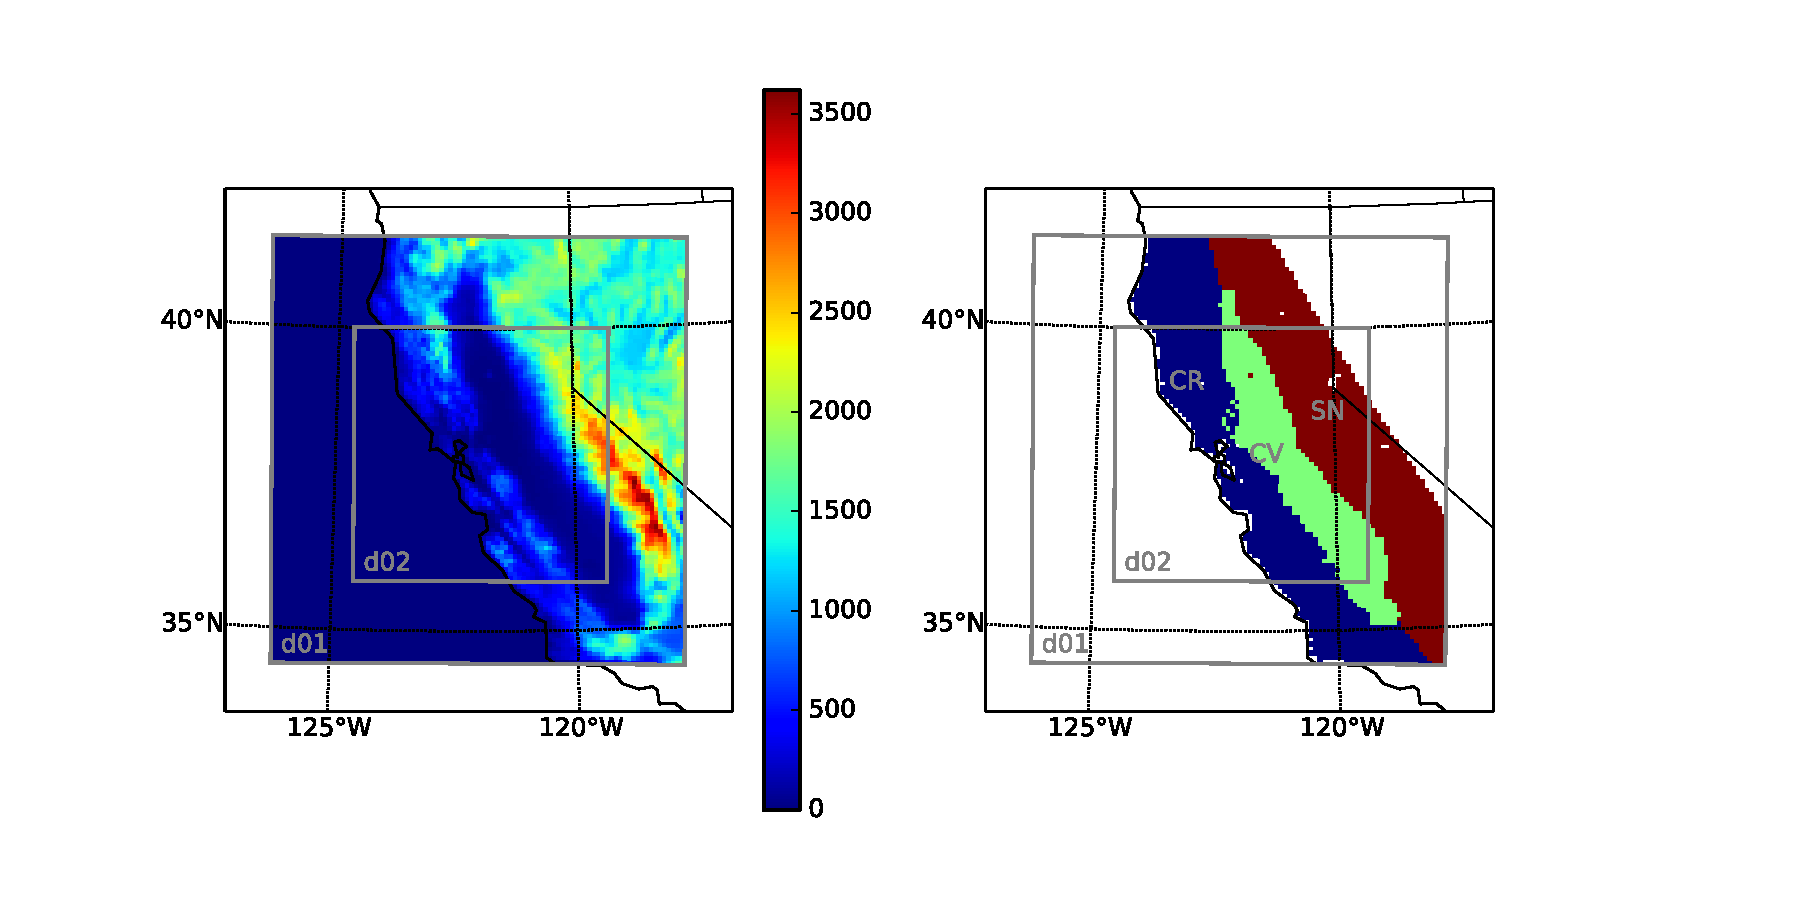
\includegraphics[width=1\textwidth]{ch3-wind/img/domain_map.pdf}
\caption{WRF model domains, showing (a) topographic height in m, and (b) regions used for soil moisture experiments in this study: the Coast Range (CR, blue), Central Valley (CV, green), and Sierra Nevada (SN, red). d01 refers to the outer model domain, and d02 refers to the inner domain.}
\label{fig:windSol_domainmap}
\end{figure}

\begin{table}
\begin{tabular}{ l c c c c c c c }
\hline
Domain & $\Delta x$ (km) & $\Delta y$ (km) & $nx$ & $ny$ & $nz$ & $\Delta t$ (s) & USGS data res \\ \hline
d01 & 8.1 & 8.1 & 96 & 99 & 45 & 45 & 2 min\\
d02 & 2.7 & 2.7 & 175 & 175 & 45 & 15 & 2 min\\
\hline
\end{tabular}
\caption{Model domains. d01 refers to the outer domain, and d02 refers to the inner domain.}
\label{table:windSol_domains}
\end{table}

In WRF, the atmospheric model is coupled to the Noah land surface model with USGS land use and soil classifications [Skamarock \textit{et al.}, 2008].  The observed distributions of land use and soil types are used, as are the default vegetation water-use parameters for each land use type [REFS], in order to simulate as closely as possible the real present day sensitivity of Solano winds to soil moisture.  Uncertainties associated with errors in the model representation of water movement in the subsurface and plant water use are addressed in the Discussion. 

As in Chapter XX, the ACM2 PBL scheme is used, following the recommendations of Marjanovic \textit{et al.} [2014] for a locally forced simple terrain case in California; this PBL scheme includes both local (small-scale turbulent) and nonlocal (large convective plume) vertical transport, and can thus simulate both stable and unstable conditions [Pleim, \textit{2007}] A LITTLE MORE DETAIL ABOUT THE PHYSICS.  The model is forced at the lateral boundaries with NCEP Eta 212 grid (40 km) operational analysis [NCEP, 1998].  Other parameterization schemes and settings are the same as those in Chapter XX Table XX.  Model variables are output every 30 minutes.

All experiments are run for the period 2009-06-26 00:00 UTC to 2009-07-11 00:00 UTC, and the first 32 hours are discarded as model spin-up.  This period was chosen for several reasons: (1) it contains a range of synoptic conditions (weak background wind June 27-July 5, and strong background wind July 6-11), (2) turbine-level wind speeds in this region are highest in the spring and summer [Zhong \textit{et al.}, 2004; Mansbach, 2010], and (3) the sensitivity to soil moisture is expected to be strongest in the warm season when radiation incident to the land surface is greatest, because changes in the relative partitioning between evapotranspiration and sensible heat flux have the largest absolute magnitude then.

\subsection{Soil moisture experiments}

The model experiments are listed in Table \ref{table:windSol_runlist}.  In the first set of experiments, we test the sensitivity of Solano winds to soil moisture in different large-scale regions of California.  In cases dryCR, dryCV, and drySN, the background volumetric soil moisture (model variable SMOIS, m$^3$ water/m$^3$ total volume) is set to 0.25, and the soil moisture of the test region (respectively, the Coast Range, Central Valley, and Sierra Nevada, shown in Figure \ref{fig:windSol_domainmap}b) is set to 0.1.  These test cases are compared with a control case where all land has soil moisture of 0.25.  In cases wetCR, wetCV, and wetSN, the background soil moisture is set to 0.1, and the soil moisture of the test region is set to 0.25.  These test cases are compared with a control case where all land has soil moisture of 0.1.

The next set of experiments tests how the Solano wind response scales with soil moisture in the Central Valley, with a normal-to-wet background in the Coast Range and Sierra Nevada.  In cases CVXX (where XX is a numeric value), the Coast Range and Sierra Nevada regions' soil moisture is set to 0.2, and the Central Valley soil moisture is set to the value specified by XX.  These test cases are compared with a control case where all land has soil moisture of 0.2.
%In cases CVXXdry, the Coast Range and Sierra Nevada regions' soil moisture is set to 0.1, and the Central Valley soil moisture again is specified by XX.

In all cases, the soil moisture is set to the prescribed values at the model start time (2009-06-26 00:00 UTC) and is reset to the prescribed value each day at 08:00 UTC (midnight Pacific Standard Time); the soil moisture evolves according to the land surface model each day between resets.  The change in soil moisture between resets is small (up to 0.02 m$^3$/m$^3$ in the regional average when soils are wet and much less when soils are dry.  Additionally, the synoptic forcing, measured by wind speed at 500 hPa, varies little between the model runs (Figure XX), and synoptic winds are weak on June 27 to July 5 and strong on July 6 to 11.  In all three regions, land surface sensible heat flux is approximately 200 W/m$^2$ greater at midday with wet soil moisture (0.25) than dry soil moisture (0.1).  \textbf{Need to make figure showing these.}

%\begin{figure}[here]
%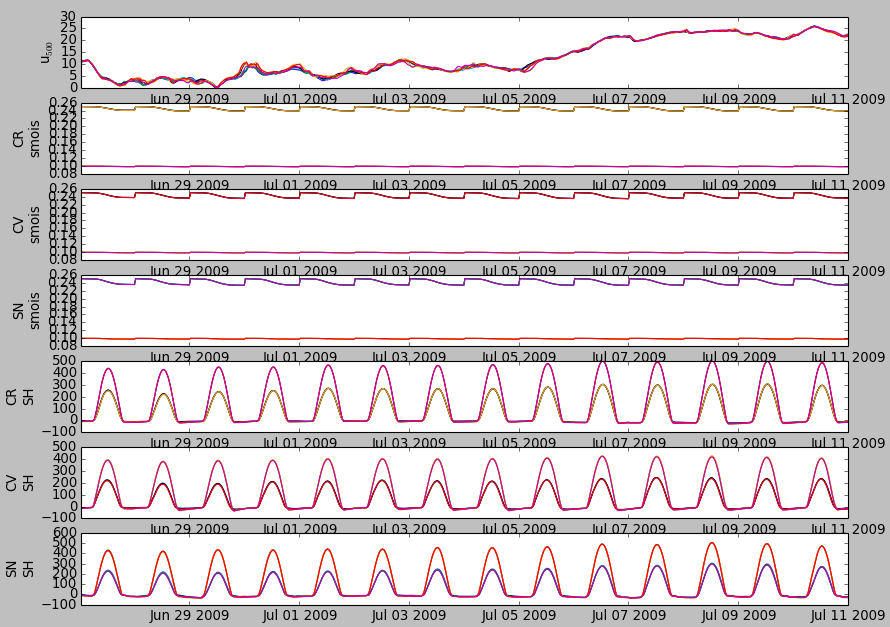
\includegraphics[width=1\textwidth]{ch3-wind/img/forcings_combo_good.png}
%\caption{Model forcing for all of the regional perturbation cases.  \textbf{I NEED ADVICE ON HOW TO DISPLAY THIS INFORMATION MORE CLEARLY AND/OR CONCISELY. Obviously, I need a legend for which color means which run.}  Top panel: wind speed over Solano at 500 hPa.  Panels 2-4: average soil moisture in the top soil layer for the CR region (panel 2), the CV region (panel 3), and the SN region (panel 4).  Panels 5-7: average surface sensible heat flux for the CR region (panel 5), the CV region (panel 6), and the SN region (panel 7).}
%\label{fig:windSol_forcings}
%\end{figure}

\begin{table}
\begin{tabular}{p{2.5cm} l p{3cm} p{3cm} p{3.5cm}}
\hline
Experiment & Run name & Background SMOIS (kg/kg) & Perturbed SMOIS region & Perturbed SMOIS value (kg/kg) \\
\hline
1 & CA-0.1 & 0.1 & none & n/a \\
1 & wetCR & 0.1 & Coast Range & 0.25 \\
1 & wetCV & 0.1 & Central Valley & 0.25 \\
1 & wetSN & 0.1 & Sierra Nevada & 0.25 \\
2 & CA-0.2 & 0.2 & none & n/a \\
2 & dryCR & 0.25 & Coast Range & 0.1 \\
2 & dryCV & 0.25 & Central Valley & 0.1 \\
2 & drySN & 0.25 & Sierra Nevada & 0.1 \\
3 & CA-0.25 & 0.25 & none & n/a \\
3 & CV0.05 & 0.2 & Central Valley & 0.05 \\
3 & CV0.1 & 0.2 & Central Valley & 0.1 \\
3 & CV0.15 & 0.2 & Central Valley & 0.15 \\
3 & CV0.25 & 0.2 & Central Valley & 0.25 \\
3 & CV0.3 & 0.2 & Central Valley & 0.3 \\
3 & CV0.35 & 0.2 & Central Valley & 0.35 \\
%CV0.05dry & 0.1 & Central Valley & 0.05 \\
%CV0.15dry & 0.1 & Central Valley & 0.15 \\
%CV0.2dry & 0.1 & Central Valley & 0.2 \\
%CV0.25dry & 0.1 & Central Valley & 0.25 \\
%CV0.3dry & 0.1 & Central Valley & 0.3 \\
%CV0.35dry & 0.1 & Central Valley & 0.35 \\
\hline
\end{tabular}
\caption{Model experiments: (1) Dry background, wet perturbation region; (2) Wet background, dry perturbation region; (3) Sensitivity to Central Valley soil moisture.}
\label{table:windSol_runlist}
\end{table}

%\end{document}


%\documentclass[12pt]{amsart}
%\usepackage{geometry} % see geometry.pdf on how to lay out the page. There's lots.
%\usepackage{datetime}
%\usepackage{setspace}
%\doublespacing
%\geometry{a4paper} % or letter or a5paper or ... etc
%% \geometry{landscape} % rotated page geometry
%
%% See the ``Article customise'' template for come common customisations
%
%\title{Wind chapter}
%\author{Percy Link}
%\date{\currenttime \ \today} % delete this line to display the current date
%
%%%% BEGIN DOCUMENT
%\begin{document}
%
%\maketitle

\section{Results}

We first characterize the differences in Solano turbine-level wind resulting from the soil moisture tests (Section \ref{subsec:CharWindChanges}).  We then investigate the physical mechanism linking changes in soil moisture to changes in Solano wind timing and magnitude (Section \ref{subsec:PhysMech}).

\subsection{Characterization of Solano wind sensitivity to soil moisture}
\label{subsec:CharWindChanges}

\subsubsection{California low-level wind system}
\label{subsubsec:control_winds}

%Before presenting the Solano winds, we quantify the synoptic and land-surface-heating forcing in each case, and we characterize the control case winds.  The synoptic forcing, measured by wind speed at 500 hPa, varies little between the model runs (Figure \ref{fig:windSol_forcings}), and synoptic winds are weak on June 27 to July 5 and strong on July 6 to 11.  In all three regions, land surface sensible heat flux is approximately 200 W/m$^2$ greater at midday with wet soil moisture (0.25) than dry soil moisture (0.1).

The low-level winds in California follow a strong diurnal cycle, driven by the diurnal cycle of the temperature difference and thus the pressure difference between land and ocean.  Regional low-level winds in the control case are consistent with previous studies of California surface winds (Figure \ref{fig:windSol_WindMapsRg} first column, Zhong \textit{et al.}, 2004; Mansbach, 2010); flow is strong through the Solano pass and splits into northward and southward branches in the Central Valley.  The southward branch is stronger than the northward branch at 06:00 and 14:00, and the northward branch strengthens at 18:00 and 00:00.  The pressure gradient from the San Francisco Bay to the Central Valley remains strong from 14:00 to 00:00 and weakens by 06:00.  \textbf{Note: I need to remake these plots to label the pressure change contours.}

\begin{figure}[here]
\includegraphics[angle=90,origin=c,width=1\textwidth]{ch3-wind/img/wind_map_regions2.eps}
\caption{Wind speed (color shading) and direction (vectors) and pressure (color contours) at 110 m ASL on the d02 domain, averaged by hour over the two-week runs.  (a)-(d) CA-0.25 control case.  (e)-(h) dryCR case, changes in wind and pressure.  (i)-(l) dryCV case, changes in wind and pressure.  (m)-(p) drySN case, changes in wind and pressure.  Top row: average for hour 06:00 for the whole run; second row: average for hour 14:00; third row: average for hour 18:00; bottom row: average for hour 00:00.}
\label{fig:windSol_WindMapsRg}
\end{figure}

\begin{figure}[here]
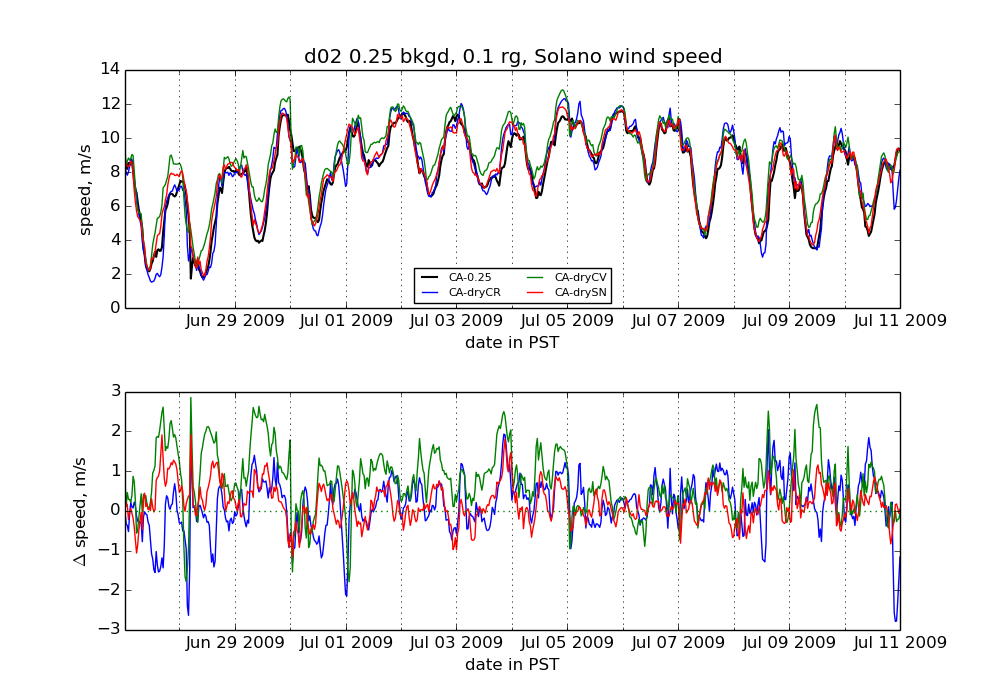
\includegraphics[width=1\textwidth]{ch3-wind/img/solano_wind_wetbkd_dryrg_d02_level0.png}
\caption{Time series of wind speed magnitude at 60 m AGL for the d02 grid point nearest the Solano wind farm, for the wet background and dry perturbation tests.  The model spin-up period is excluded.}
\label{fig:windSol_TseriesDryRg}
\end{figure}

\begin{figure}[here]
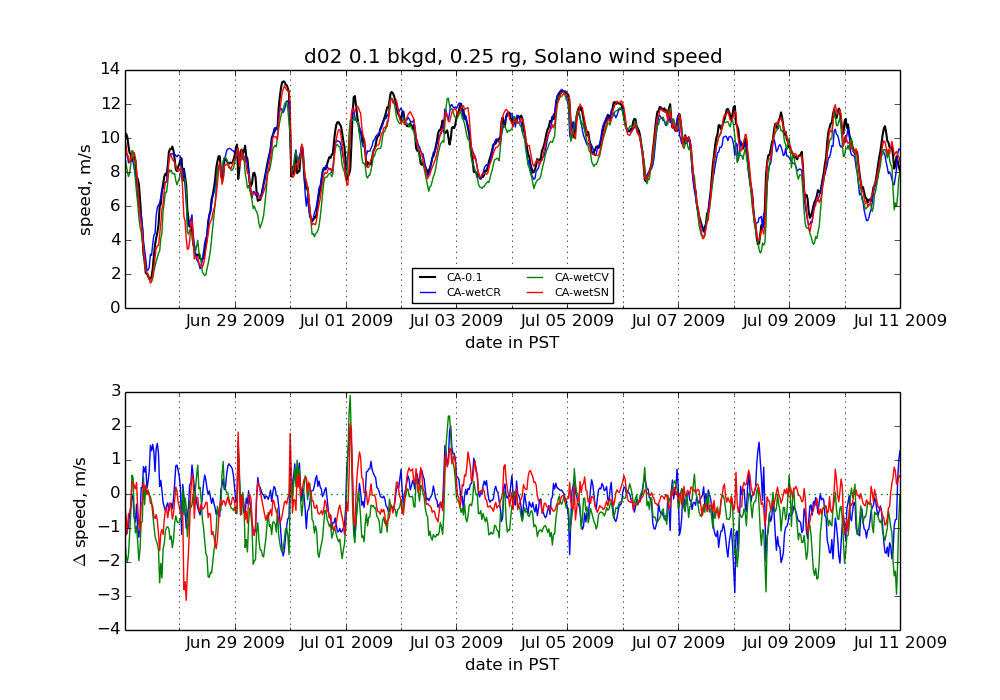
\includegraphics[width=1\textwidth]{ch3-wind/img/solano_wind_drybkd_wetrg_d02_level0.png}
\caption{Time series of wind speed magnitude at 60 m AGL for the d02 grid point nearest the Solano wind farm, for the dry background and wet perturbation tests.  The model spin-up period is excluded.}
\label{fig:windSol_TseriesWetRg}
\end{figure}

Similarly, wind at Solano has a strong diurnal cycle (Figures \ref{fig:windSol_TseriesDryRg}(a) and \ref{fig:windSol_TseriesWetRg}(a)); notably, the surface wind speed does not track the 500 hPa synoptic wind in this period (cf. Figure \ref{fig:windSol_forcings}) but rather is dominated by the diurnal signal.  Solano wind speeds are greatest at night (19:00 to 03:00) and weakest in the morning (08:00 to 13:00; Figure \ref{fig:windSol_DiffDiurnalDryRg}(a) and Figure \ref{fig:windSol_DiffDiurnalWetRg}(a))  There is a pronounced low-level ($\le$300 m) peak in Solano winds that is particularly pronounced at night (Figure \ref{fig:windSol_VertProfileDryRg}(a)).

\begin{figure}[here]
\begin{subfigure}{0.5\textwidth}
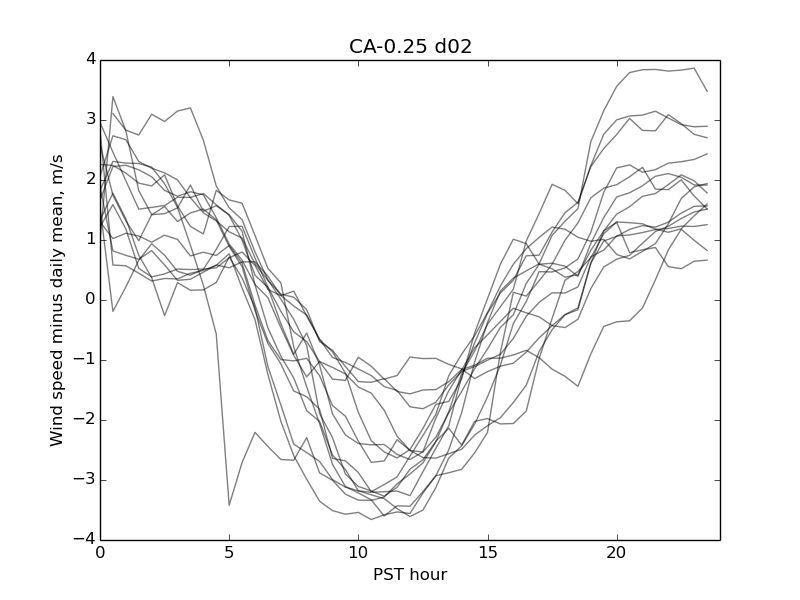
\includegraphics[width=1\textwidth]{ch3-wind/img/solano_controlwind_minusmean_CA0pt25_d02_level0.png}
\caption{}
\end{subfigure}
\begin{subfigure}{0.5\textwidth}
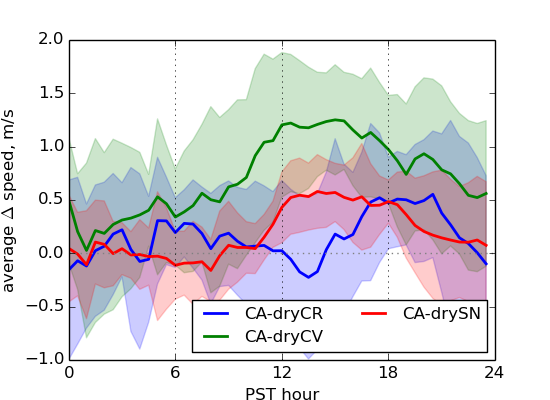
\includegraphics[width=1\textwidth]{ch3-wind/img/solano_diurnalwind_dry_regions_d02_level0.png}
\caption{}
\end{subfigure}
\caption{(a) Overlaid diurnal cycles of wind speed magnitude minus daily mean wind speed, at 60 m AGL for the d02 grid point nearest the Solano wind farm, for the CA-0.25 control case.  (b) Diurnally averaged differences in wind speed, at 60 m AGL for the d02 grid point nearest the Solano wind farm, for the wet background/dry perturbation cases.  Shading represents one standard deviation.}
\label{fig:windSol_DiffDiurnalDryRg}
\end{figure}

\begin{figure}[here]
\begin{subfigure}{0.5\textwidth}
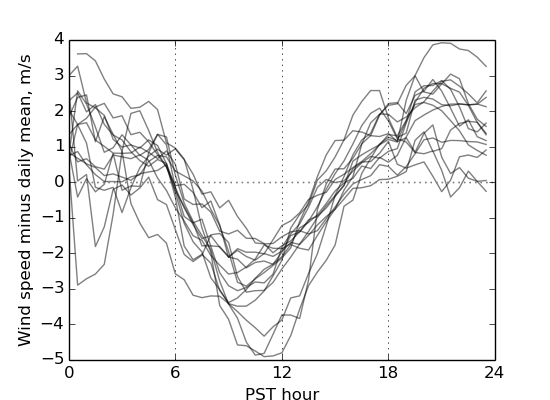
\includegraphics[width=1\textwidth]{ch3-wind/img/solano_controlwind_minusmean_CA0pt1_d02_level0.png}
\caption{}
\end{subfigure}
\begin{subfigure}{0.5\textwidth}
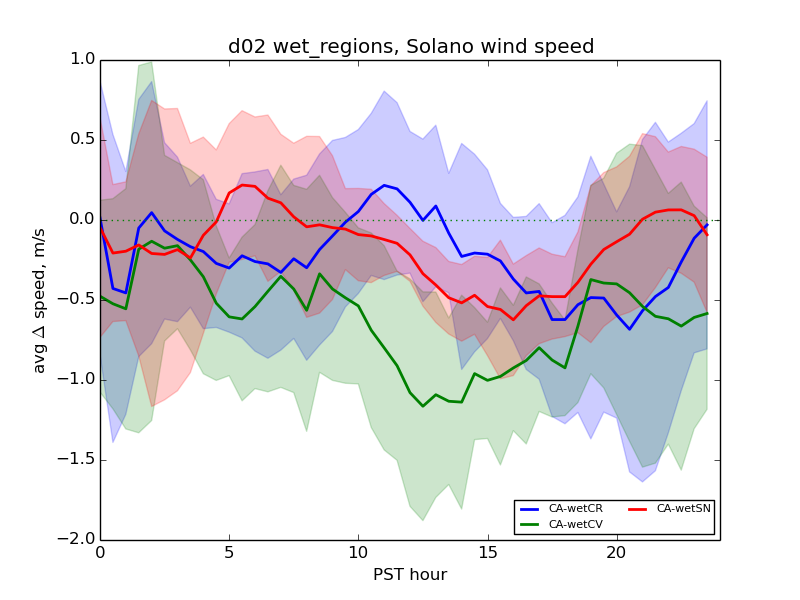
\includegraphics[width=1\textwidth]{ch3-wind/img/solano_diurnalwind_wet_regions_d02_level0.png}
\caption{}
\end{subfigure}
\caption{(a) Overlaid diurnal cycles of wind speed magnitude minus daily mean wind speed, at 60 m AGL for the d02 grid point nearest the Solano wind farm, for the CA-0.1 control case.  (b) Diurnally averaged differences in wind speed, at 60 m AGL for the d02 grid point nearest the Solano wind farm, for the dry background/wet perturbation cases.  Shading represents one standard deviation.}
\label{fig:windSol_DiffDiurnalWetRg}
\end{figure}

\begin{figure}[here]
\begin{subfigure}{0.49\textwidth}
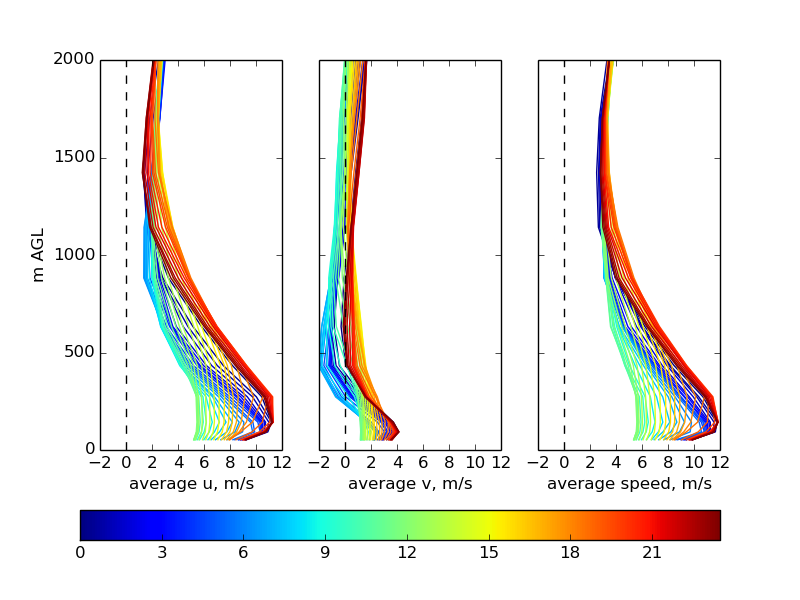
\includegraphics[width=\textwidth]{ch3-wind/img/windprof_hr_avg_CA0pt25.png}
\caption{}
\end{subfigure}
\begin{subfigure}{0.49\textwidth}
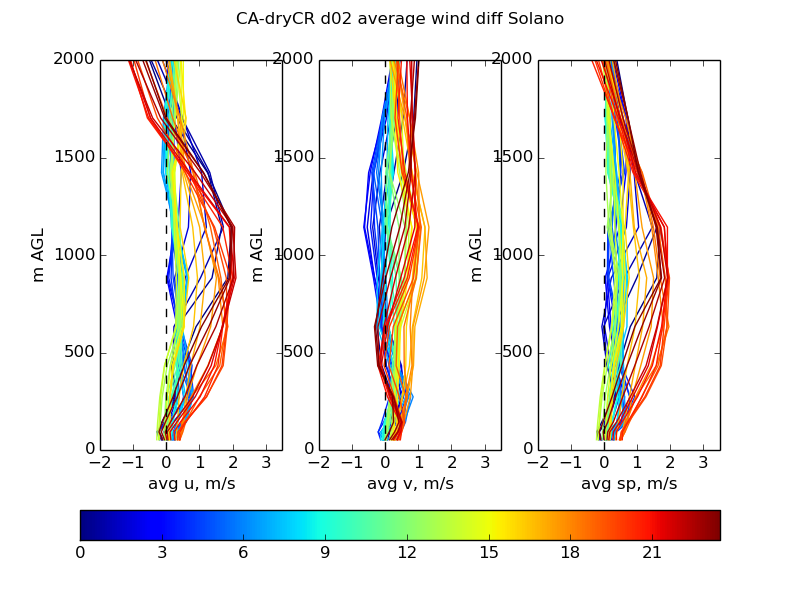
\includegraphics[width=\textwidth]{ch3-wind/img/windprof_diff_hr_avg_dryCR.png}
\caption{}
\end{subfigure}
\begin{subfigure}{0.49\textwidth}
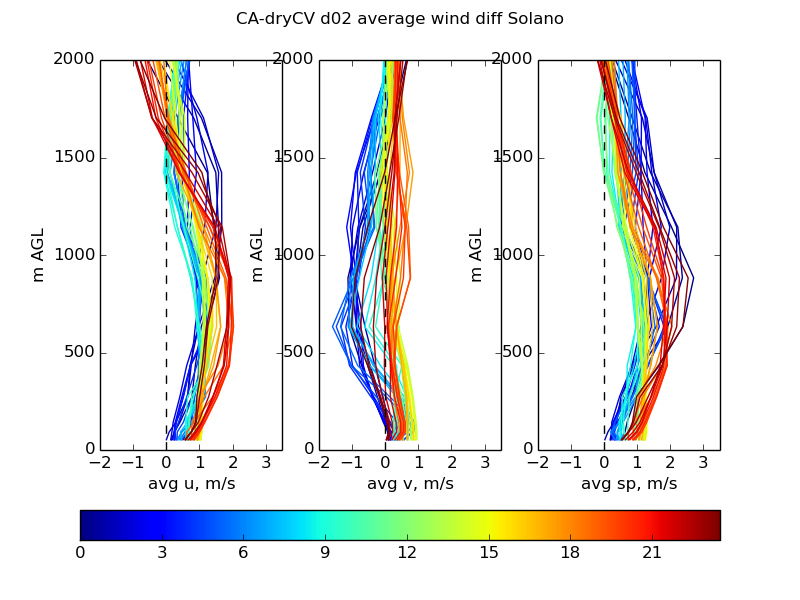
\includegraphics[width=\textwidth]{ch3-wind/img/windprof_diff_hr_avg_dryCV.png}
\caption{}
\end{subfigure}
\begin{subfigure}{0.49\textwidth}
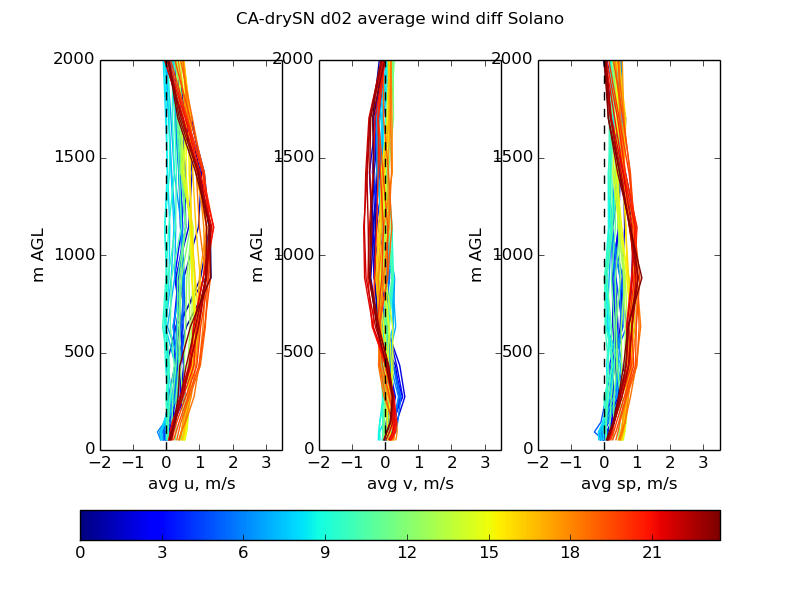
\includegraphics[width=\textwidth]{ch3-wind/img/windprof_diff_hr_avg_drySN.png}
\caption{}
\end{subfigure}
\caption{Vertical profiles of $u$, $v$, and $|u|$, averaged by time of day over the whole simulation (colorbar indicates hour of day in local time), for (a) CA-0.25 control run, and averaged differences from control run for the dry regional test cases: (b) dryCR, (c) dryCV, (d) drySN.}
\label{fig:windSol_VertProfileDryRg}
\end{figure}

\subsubsection{Regional sensitivity}

The Solano wind changes occur in the context of larger regional wind and pressure changes (Figure \ref{fig:windSol_WindMapsRg}).  In all dry regional tests, the pressure gradient and wind increase throughout the Central Valley, most strongly in the afternoon (second and third rows in Figure \ref{fig:windSol_WindMapsRg}).  In the dry Coast Range test (Figure \ref{fig:windSol_WindMapsRg} (e)-(h)), the pressure in the northern Central Valley decreases and wind in the northern Central Valley strengthens as cyclonic flow develops around the northern Coast Range.  In the dry Central Valley test (Figure \ref{fig:windSol_WindMapsRg} (i)-(l)), the pressure gradient from the San Francisco Bay to the Central Valley increases dramatically at 14:00, and these increases persist at 18:00 and to a lesser degree at 00:00. However, at 18:00, the zone of steepest pressure change has been pushed further eastward, and the strongest wind increases track this band of largest pressure gradient.  The pattern of wind increases at 00:00 is disorganized, and wind speeds decrease in the southern Central Valley at 06:00.  In the dry Sierra Nevada case (Figure \ref{fig:windSol_WindMapsRg} (m)-(p)), the pressure gradient strengthens moderately at 14:00 and 18:00, but pressure changes are minimal by 00:00 and 06:00.  Wind speeds increase through the Solano pass and the middle Central Valley in the afternoon (14:00 and 18:00), and by 18:00, the bands of largest wind increases have moved outward along Central Valley, again following zones of greatest pressure gradient increase.  Wind changes at night (00:00 and 06:00) are small and disorganized.

%The Solano wind in the regional test cases differs from the control case by as much as 2 m/s, and the largest changes occur when Central Valley soil moisture is perturbed (dryCV and wetCV).  

For all regional test cases, drier soils on a wet background increase Solano winds in the afternoon and evening relative to the all-wet control (Figure \ref{fig:windSol_DiffDiurnalDryRg}(b)); this increase is largest in the dryCV case.  The increases in both the dryCV and drySN cases are greatest between 11:00 and 18:00 (0.8-1.8 m/s for dryCV and 0.25-0.8 m/s for drySN), while the increase in the dryCR case happens later, between 17:00 and 22:00 (0.25-1 m/s).  Importantly, increases in the afternoon cause the daily wind speed ramp-up to shift earlier, because the increases occur at the same time as the control ramp-up (Figure \ref{fig:windSol_DiffDiurnalDryRg}(a)).  Because there are no corresponding decreases at the hour of ramp-down, this means that the duration of the high-wind period also increases.  Also, drier soils (especially in the Central Valley) increase the minimum wind (08:00 to 13:00) on many individual days (Figure \ref{fig:windSol_TseriesDryRg}), but the average increases in the minimum wind are not more than one standard deviation greater than zero in the two-week average diurnal cycle (Figure \ref{fig:windSol_DiffDiurnalDryRg}(b)).

Wetter soils on a dry background cause winds to decrease relative to the all-dry control case, and the magnitudes of the decreases are similar to the magnitudes of the increases in the dry regional tests (Figure \ref{fig:windSol_DiffDiurnalWetRg}(b)).  Again, the decrease is largest in when Central Valley soil moisture is perturbed.  Both the wetCV and wetSN cases have wind decreases during 10:00-18:00 that are more than one standard deviation from zero (0.5-1.8 m/s for wetCV and 0.25-0.8 m/s for wetSN); for the wetCR case, there are no times of day with wind changes more than one standard deviation from zero, although there are weak decreases in the late afternoon and evening.

In summary, the Central Valley soil moisture influences the Solano turbine-level winds more strongly than does the Coast Range or Sierra Nevada soil moisture.  Drier soils in all regions, but especially in the Central Valley, increase Solano wind speeds during ramp-up and peak hours (afternoon and evening); drier soils in the Central Valley, especially, shift the daily wind ramp-up earlier.  Conversely, wetter Central Valley soils cause Solano winds to decrease during ramp-up and peak times.

\subsubsection{Scaling of wind changes with Central Valley soil moisture}

\begin{figure}[here]
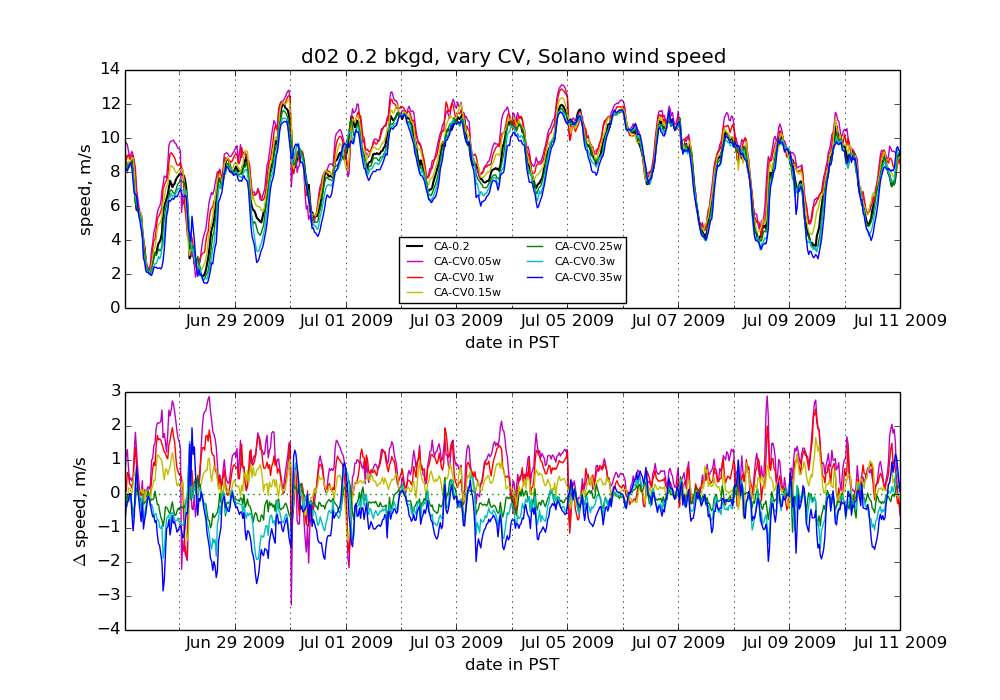
\includegraphics[width=1\textwidth]{ch3-wind/img/solano_wind_CV0pt2_d02_level0.png}
\caption{Time series of wind speed magnitude at 60 m AGL for the d02 grid point nearest the Solano wind farm, for a range of Central Valley soil moisture values, with soil moisture = 0.2 in the Coast Range and Sierra Nevada.  (a) Wind speed time series, (b) time series of differences between test cases and control (CA-0.2).  The model spin-up period is excluded.}
\label{fig:windSol_TseriesWindCV}
\end{figure}

\begin{figure}[here]
\begin{subfigure}{0.6\textwidth}
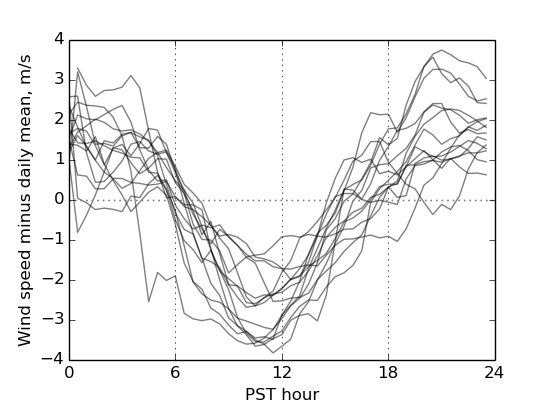
\includegraphics[width=1\textwidth]{ch3-wind/img/solano_controlwind_minusmean_CA0pt2_d02_level0.png}
\caption{}
\end{subfigure}
\begin{subfigure}{0.6\textwidth}
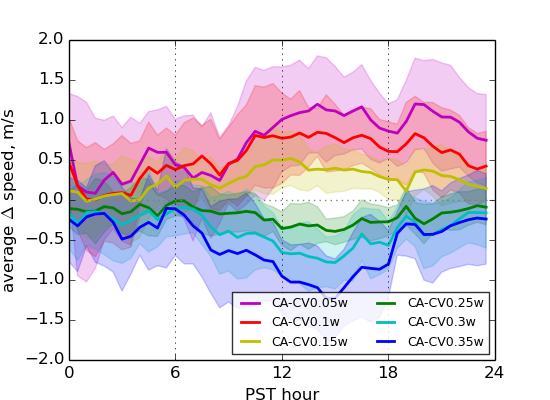
\includegraphics[width=1\textwidth]{ch3-wind/img/solano_diurnalwind_CV_0pt2_d02_level0.png}
\caption{}
\end{subfigure}
\caption{(a) Overlaid diurnal cycles of wind speed magnitude minus daily mean wind speed, at 60 m AGL for the d02 grid point nearest the Solano wind farm, for the CA-0.2 control case.  (b) Diurnally averaged differences in wind speed, at 60 m AGL for the d02 grid point nearest the Solano wind farm, for a range of Central Valley soil moisture values.  Shading represents one standard deviation.}
\label{fig:windSol_DiffDiurnalCV0pt2}
\end{figure}

\begin{figure}[here]
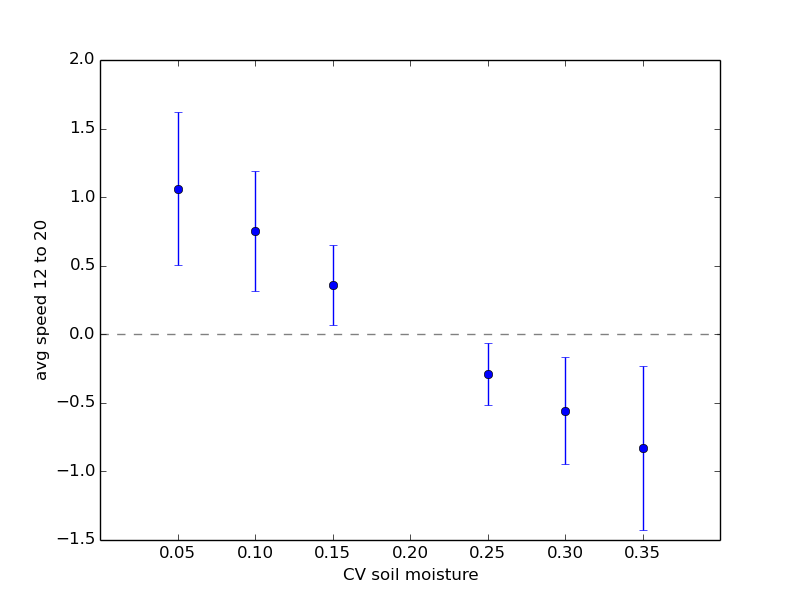
\includegraphics[width=1\textwidth]{ch3-wind/img/shifts_CVsmois_12-20_d02.png}
\caption{Average changes in wind speed between hours 12:00 and 20:00, for different values of CV soil moisture with CR and SN soil moisture set to 0.2 m$^3$/m$^3$.  Changes are relative to the CA-0.2 control case.  Error bars represent one standard deviation.}
\label{fig:windSol_ShiftsMaxCV}
\end{figure}

Drier Central Valley soils increase Solano winds, while wetter Central Valley soils decrease Solano winds, relative to the moderately wet control of soil moisture = 0.2 (Figure \ref{fig:windSol_TseriesWindCV}.)  These changes can be up to 3 m/s, and they occur most consistently in the hours of 12:00 to 22:00 (Figure \ref{fig:windSol_DiffDiurnalCV0pt2}(b)), when they are 0.8-1.7 m/s on average in the driest Central Valley case (CV0.05).  The average changes during hours 12:00 to 22:00 scale slightly nonlinearly with CV soil moisture (Figure \ref{fig:windSol_ShiftsMaxCV}), with larger increases in wind per unit soil moisture decrease when the Central Valley soil is drier than 0.2 m$^3$/m$^3$.  The greater sensitivity of wind to soil moisture when soils are drier may be due to a greater sensitivity of surface heating to soil moisture when soils are drier, because of rapid declines in soil hydraulic conductivity and plant stomatal conductance in the moderate-to-dry soil moisture range (\textbf{cite something � Bonan? Sap flow paper? Transitional soil moisture regime paper of some kind?}).

\clearpage

\subsection{Physical mechanism}
\label{subsec:PhysMech}

Next we investigate the physical mechanism by which changes in soil moisture, especially in the Central Valley, influence near-surface winds at Solano.  

The strong diurnal component of the Solano wind (Figures \ref{fig:windSol_TseriesDryRg} and \ref{fig:windSol_TseriesWetRg}) and the wind speed peak at low levels (Figure \ref{fig:windSol_VertProfileDryRg}) suggest significant forcing by land surface heating (consistent with Zhong \textit{et al.} [2004] and Mansbach [2010]).  In order to explore the influence of land surface forcing on terms in the momentum budget, we model the topographically channeled wind at Solano as simple one-dimensional flow through the pass governed by a one-dimensional momentum equation,

\begin{equation}
\frac{\partial u}{\partial t} = -u\frac{\partial u}{\partial x} -\frac{1}{\rho} \frac{\partial p}{\partial x} - F\left(\frac{\partial u}{\partial z}, N\right),
\label{eqn:windSol_momentum}
\end{equation}
neglecting the Coriolis term because of the topographic constraint on wind direction.  The first term on the right hand side is the advection of momentum, the second term is the pressure gradient force, and the third term is frictional dissipation as an unspecified function of vertical wind shear and stability (quantified by $N$, the Brunt-V\"ais\"al\"a frequency).  We are interested in the importance of each of these terms through the diurnal cycle and in the influence of soil moisture changes on each of these terms.

\subsubsection{Driving pressure gradient}

\begin{figure}[here]
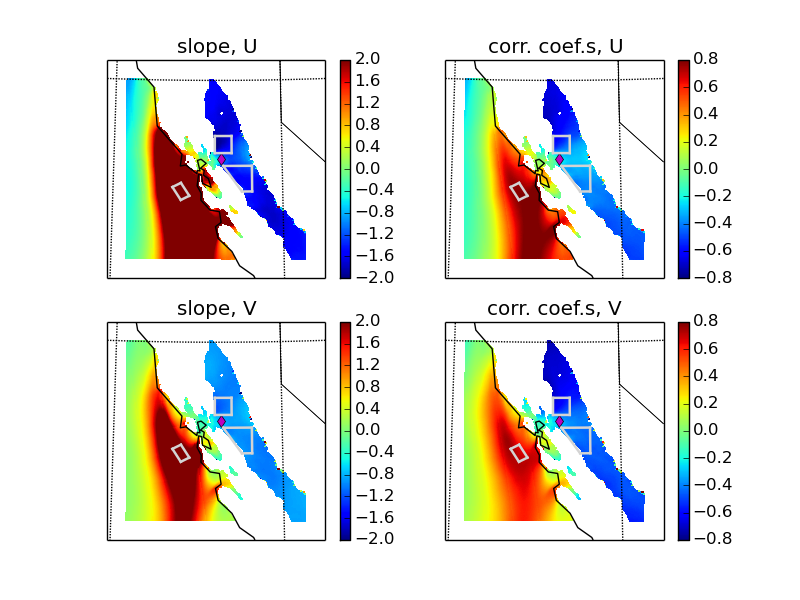
\includegraphics[width=1\textwidth]{ch3-wind/img/corr_wind_panom_lev110_lag12_CA0pt25.png}
\caption{CA-0.25 case: Solano 60 m AGL (110 m ASL) wind linearly regressed against horizontal pressure anomaly at 110 m ASL, with wind lagging pressure by 6 hours.  Top row: $u$-component of wind; bottom row: $v$-component of wind.  Left column: linear regression slope; right column: correlation coefficient.  Gray boxes outline areas used to calculate pressure gradients; ocean box is ``OCN", northern box in the Central valley is ``NCV", and southern box in Central Valley is ``SCV".}
\label{fig:windSol_CorrMap0pt25}
\end{figure}

\begin{figure}[here]
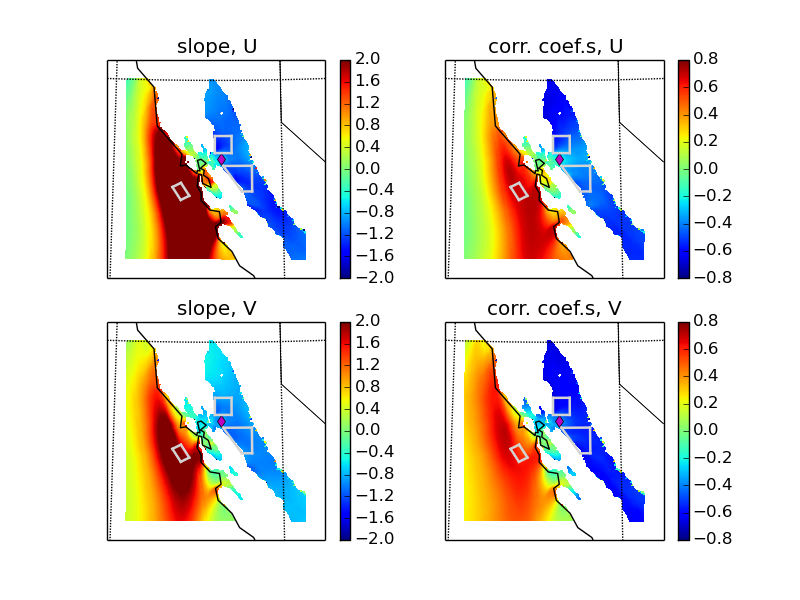
\includegraphics[width=1\textwidth]{ch3-wind/img/corr_wind_panom_lev110_lag12_CA0pt1.png}
\caption{CA-0.1 case: Solano 60 m AGL (110 m ASL) wind linearly regressed against horizontal pressure anomaly at 110 m ASL, with wind lagging pressure by 6 hours.  Top row: $u$-component of wind; bottom row: $v$-component of wind.  Left column: linear regression slope; right column: correlation coefficient.}
\label{fig:windSol_CorrMap0pt1}
\end{figure}

In order to identify the pressure gradient most relevant to Solano winds, we linearly regress the horizontal pressure anomaly, calculated at each output time step, against Solano turbine-level wind.  The regression is repeated for pressure at a range of heights and for a range of lag times, with wind lagging pressure.  The regression slopes and correlation coefficients for the control cases (CA-0.25, Figure \ref{fig:windSol_CorrMap0pt25}, and CA-0.1, Figure \ref{fig:windSol_CorrMap0pt1}) show a consistent pattern of positive slopes and correlation coefficients over the ocean near the central coast (meaning higher pressure in those regions corresponds to faster wind), and negative slopes and correlation coefficients throughout the Central Valley, especially just north and south of the Solano pass (meaning lower pressure in those regions corresponds to faster wind).

\begin{figure}[here]
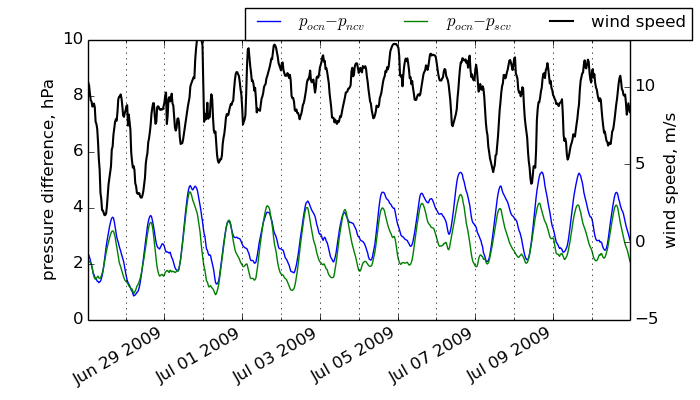
\includegraphics[width=1\textwidth]{ch3-wind/img/pgrad_wind_CA0pt1_level110.png}
\caption{CA-0.1 control case: Solano 60 m AGL (110 m ASL) wind (black) and average pressure difference OCN box minus NCV box (blue) and OCN box minus SCV box (green) at 110 m ASL.  The sign of the pressure difference is chosen to correspond with the $\frac{-1}{\rho} \frac{\partial p}{\partial x}$ term in the momentum budget.}
\label{fig:windSol_PgradWind}
\end{figure}

\begin{figure}[here]
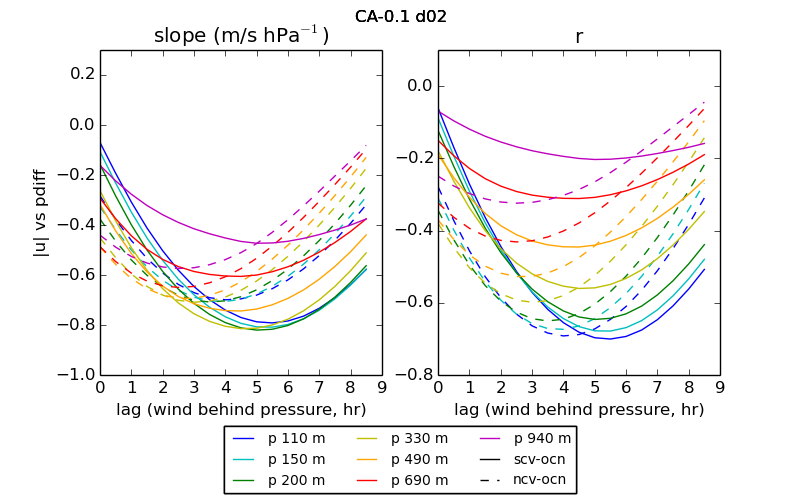
\includegraphics[width=1\textwidth]{ch3-wind/img/lag_corr_pdiff_combo_ncv_scv_d02_CA0pt1.png}
\caption{CA-0.1 control case: lagged linear regression of Solano 60 m AGL (110 m ASL) wind against average pressure difference NCV box minus OCN box (dashed) and SCV box minus OCN box (solid).  Correlations are only shown for speed, because u and v velocity component results are very similar.}
\label{fig:windSol_LagCorrCtrl}
\end{figure}

Based on this finding, we choose three boxes, shown in gray in Figures \ref{fig:windSol_CorrMap0pt25} to \ref{fig:windSol_CorrMap0pt1}, to represent the pressure gradient driving Solano winds.  The lag of wind speed behind pressure gradient is evident in the time series of Solano wind and pressure difference between the boxes (Figure \ref{fig:windSol_PgradWind}).  Not only does the pressure difference peak 5-6 hours before the Solano wind speed, but the peak pressure difference rapidly dissipates (beginning to decline after 1-2 hours), while the peak wind speed persists for 6-8 hours.  Using the pressure difference between the three boxes, we confirm that the peak sensitivity (as measured by the regression slope) and correlation occur with pressure at 110 m ASL (although the metrics are high at all levels below $\sim$300 m) with a lag of $\sim$4-5 hr for NCV-OCN pressure and $\sim$5-6.5 hr for SCV-OCN pressure (Figure \ref{fig:windSol_LagCorrCtrl}).

\begin{figure}[here]
\begin{subfigure}{0.6\textwidth}
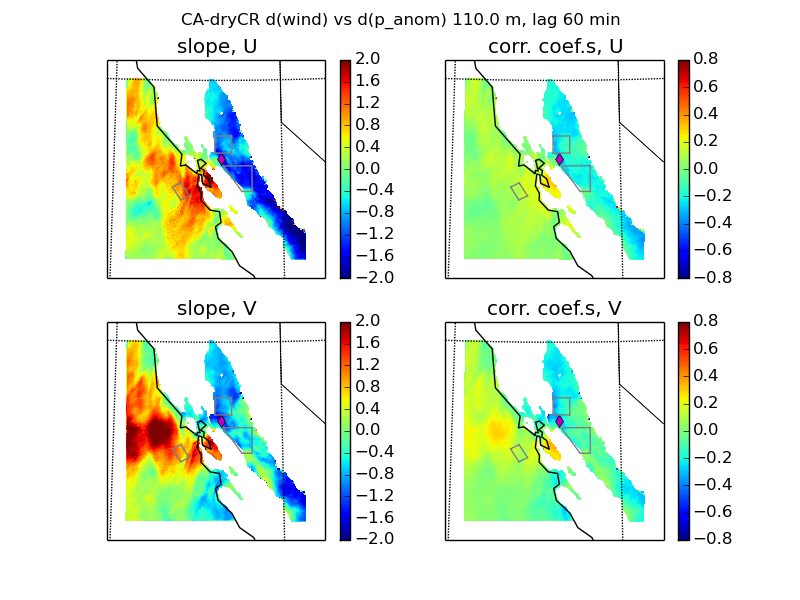
\includegraphics[width=\textwidth]{ch3-wind/img/corr_dwind_dpanom_lev110_lag2_dryCR.png}
\caption{}
\end{subfigure}
\begin{subfigure}{0.6\textwidth}
\includegraphics[width=\textwidth]{ch3-wind/img/corr_dwind_dpanom_lev110_lag2_dryCV.png}
\caption{}
\end{subfigure}
\begin{subfigure}{0.6\textwidth}
\includegraphics[width=\textwidth]{ch3-wind/img/corr_dwind_dpanom_lev110_lag2_drySN.png}
\caption{}
\end{subfigure}
\caption{Correlation between Solano wind changes at 60 m AGL and horizontal pressure anomaly of change in 110 m ASL pressure, with a lag of 60 min, for the dry regional test cases minus control: (a) dryCR, (b) dryCV, (c) drySN.  The order of panels is as in Figure \ref{fig:windSol_CorrMap0pt25}.}
\label{fig:windSol_CorrMapDryRg}
\end{figure}

\begin{figure}[here]
\begin{subfigure}{0.6\textwidth}
\includegraphics[width=\textwidth]{ch3-wind/img/corr_dwind_dpanom_lev110_lag2_wetCR.png}
\caption{}
\end{subfigure}
\begin{subfigure}{0.6\textwidth}
\includegraphics[width=\textwidth]{ch3-wind/img/corr_dwind_dpanom_lev110_lag2_wetCV.png}
\caption{}
\end{subfigure}
\begin{subfigure}{0.6\textwidth}
\includegraphics[width=\textwidth]{ch3-wind/img/corr_dwind_dpanom_lev110_lag2_wetSN.png}
\caption{}
\end{subfigure}
\caption{Correlation between Solano wind changes at 60 m AGL and horizontal pressure anomaly of change in 110 m ASL pressure, with a lag of 60 min, for the wet regional test cases minus control: (a) wetCR, (b) wetCV, (c) wetSN.  The order of panels is as in Figure \ref{fig:windSol_CorrMap0pt25}.}
\label{fig:windSol_CorrMapWetRg}
\end{figure}

\begin{figure}[here]
\includegraphics[width=1\textwidth]{ch3-wind/img/lag_corr_dpdiff_combo_ncv_scv_d02_testminusctrl.png}
\caption{Dry regional perturbation cases: lagged linear regression of test-minus-control Solano 60 m AGL (110 m ASL) wind against test-minus-control average pressure difference NCV box minus OCN box (dashed) and SCV box minus OCN box (solid).  Top row: dryCR; middle row: dryCV; bottom row: drySN.}
\label{fig:windSol_LagCorrTest}
\end{figure}

Repeating the regression analysis using test-minus-control changes in pressure and Solano wind, a similar spatial pattern of sensitivity emerges (positive correlation between Solano wind changes and pressure changes in the central coastal ocean, and negative correlation between Solano wind changes and pressure changes in the Central Valley), albeit with weaker correlation (Figures \ref{fig:windSol_CorrMapDryRg} and \ref{fig:windSol_CorrMapWetRg}).  Again, the changes in wind speed correlate maximally with the changes in pressure at the lowest altitudes ($\le$ 200 m, Figure \ref{fig:windSol_LagCorrTest}).  In contrast to the control cases which have a 5-6 hour lag, the test-minus-control changes correlate maximally at a lag of $\le$ 1 hour (Figure \ref{fig:windSol_LagCorrTest}).

\subsubsection{Temperature controls on pressure}

\begin{figure}[here]
\includegraphics[width=0.9\textwidth]{ch3-wind/img/timeheight_T_pdiff_ocnbox_ncvbox_0pt25.png}
\caption{CA-0.25 control case: Temporal evolution of the vertical profile of temperature for the OCN box (top panel), the NCV box (second panel), NCV minus OCN (third panel); and time series of the NCV minus OCN pressure at 110 m ASL (bottom panel).  White areas indicate times when the lowest $\sigma$ model level was higher than 30 m ASL for the NCV box.}
\label{fig:windSol_TimeHeightCtrl}
\end{figure}

The diurnal variations in low-level pressure correspond to diurnal variations in boundary layer temperature, because pressure is the vertical integral of the weight of the air column above a point, and changes in temperature change the density and thus the weight of the air column.  Diurnal temperature variations are larger in the Central Valley than over the ocean (Figure \ref{fig:windSol_TimeHeightCtrl}).  In the NCV box, the temperature near the surface (\textless 100 m ASL) declines quickly after sunset, but the temperature aloft in the boundary layer (particularly 300-700 m) remains elevated until at least midnight (Figure \ref{fig:windSol_TimeHeightCtrl}, panel 2).  Both the NCV temperature and the NCV-OCN temperature difference peak around 17:00.  The temperature difference at low levels (\textless 110 m) drops after sunset and approaches zero in the early morning some days, but the temperature difference remains positive at 110-490 m on most days, with NCV warmer than OCN by up to 12 deg C even in the early morning.  The near-surface cooling in the Central Valley is due to a combination of radiative cooling of the land surface and advection of cooler marine air by the low-level wind maximum.  The pressure difference is most negative (strongest gradient) at the same time as the maximum temperature difference, around 17:00, and is smallest in magnitude (weakest gradient) just before sunrise, around 06:00, when the NCV boundary layer is coolest.  

\begin{figure}[here]
\includegraphics[width=0.9\textwidth]{ch3-wind/img/timeheight_T_pdiff_ocnbox_ncvbox_diff_dryCV.png}
\caption{dryCV case: Temporal evolution of the vertical profile of test-minus-control temperature changes for the OCN box (top panel), the NCV box (second panel), NCV minus OCN (third panel); and time series of test-minus-control changes in the NCV minus OCN pressure at 110 m ASL (bottom panel).  White areas indicate times when the lowest $\sigma$ model level was higher than 30 m ASL for the NCV box.}
\label{fig:windSol_TimeHeightDryCV}
\end{figure}

Changes in soil moisture affect the pressure gradient by changing surface heat fluxes and thus air temperature.  Temperature changes in the lower 1000 m of the NCV box are much larger in the dryCV case than in the dryCR or drySN cases; as such, only the dryCV case is shown (Figure \ref{fig:windSol_TimeHeightDryCV}).  We note that in the dryCR and drySN cases, temperature and pressure changes are much smaller (+/- 1 degree C and -0.4 hPa), and the pressure gradient strengthens in the late afternoon, largely corresponding to warming at boundary layer levels above the surface (150 m to 1200 m).

In the dryCV case, the NCV experiences strong low-level heating beginning in the morning, increasing in altitude as the boundary layer grows; temperature increases during day are well-mixed in the boundary layer.  There is mild cooling over the OCN box at 200-330 m in the first week of the simulation.  The strongest increase in temperature difference (warming of NCV relative to OCN) occurs late morning to late afternoon, at all levels below 690 m.  At night, there is a small decrease in the low-level (\textless 330 m) temperature difference.  The corresponding strengthening of the pressure difference is also greatest from late morning to late afternoon.  The mild strengthening of the pressure gradient on some nights (e.g. early morning of June 28, June 29, July 3, July 8) appears related to longer nocturnal persistence of warming at NCV relative to OCN in the residual boundary layer (150 m - 690 m, although the elevation of warming differs among individual days).

\subsubsection{Momentum budget timing and changes}

\begin{figure}[here]
\includegraphics[width=0.9\textwidth]{ch3-wind/img/momentum_terms_diurnal_0pt25.png}
\caption{CA-0.25 control case: Diurnal average of terms of the momentum balance.  Pressure gradient is calculated between the NCV and OCN boxes, and using density calculated at Solano 60 m AGL.  Advection is calculated as $u_{solano}\frac{\partial u}{\partial x}$ with $\frac{\partial u}{\partial x}$ estimated with the gradient in wind between Solano and San Pablo Bay (the northern part of the San Francisco Bay).  $\frac{\partial u}{\partial t}$ is calculated using Solano 60 m AGL wind speed.  Friction (cyan) is calculated as the residual of the other three terms, following Equation \ref{eqn:windSol_momentum}.  Shading represents one standard deviation.}
\label{fig:windSol_MomTermsDiurn}
\end{figure}

The momentum advection, pressure gradient, and $u$ time tendency terms in Equation \ref{eqn:windSol_momentum} are estimated from model output for the CA-0.25 control (Figure \ref{fig:windSol_MomTermsDiurn}).  Using these three model-derived terms, we calculate the friction term as the residual (Figure \ref{fig:windSol_MomTermsDiurn}, cyan line).  The friction term has to vary diurnally in order to reproduce the observed wind diurnal cycle.  The time tendency ($\frac{\partial u}{\partial t}$) term is much smaller than pressure gradient term, even in afternoon when the pressure gradient is largest and advection is small.  If friction were not also large at this time, the wind would accelerate much faster.  Conversely, high wind speeds persist even after the pressure gradient declines between 22:00 and 04:00 and despite the strong advection of lower momentum air.  If friction during the night remained at its high afternoon values, the winds would decelerate at night.  The decline in the friction term at night is necessary in order to explain the observed high winds at night.  [\textbf{cite LLJ paper of some sort - not the first time this is being said.}]  Moreover, this residual has the expected diurnal shape of friction, with high values in the daytime when convective turbulence creates a uniform boundary layer and high momentum flux to the ground, and low values at night when the residual upper boundary layer decouples from the shallow stable nocturnal boundary layer and is buffered from friction with the surface.
% Indeed, the diurnal course of modeled $u*$ at Solano has the same timing as the $F(\frac{\partial u}{\partial z}, N)$ term calculated from the residual (ustar figure).

\begin{figure}[here]
\includegraphics[width=0.9\textwidth]{ch3-wind/img/momentum_terms_diurnal_diff_dryCV.png}
\caption{dryCV case: Diurnal average of test-minus-control change in terms of the momentum balance, calculated as in Figure \ref{fig:windSol_MomTermsDiurn}.  Shading represents one standard deviation.}
\label{fig:windSol_MomTermsDiurnDiff}
\end{figure}

In the dryCV case, the pressure gradient term increases at all hours but especially between 10:00 and 18:00 (Figure \ref{fig:windSol_MomTermsDiurnDiff}), when it increases by 20\% to 30\% (cf. Figure \ref{fig:windSol_MomTermsDiurn}).  The advection term becomes more negative at those same hours, as faster Solano wind transports lower momentum air more effectively.  The friction term also becomes more negative in the daytime, probably due to greater instability and convection from the hotter Central Valley land surface.  The changes in the dryCR and drySN cases were much smaller, with the pressure gradient term increasing by a maximum of 0.0001 to 0.0002 m/s$^2$ in the late afternoon.

\subsubsection{Summary of mechanism}
Solano wind responds to the near-surface pressure gradient between the Central Valley near the Solano pass and the central coast ocean.  Changes in boundary layer temperature at either of these locations influences this driving pressure gradient.  Soil moisture strongly influences land surface heating, and changes to soil moisture in the Central Valley strongly affect boundary layer temperature and thus near-surface pressure in the regions relevant to the Solano wind.  When Central Valley soils are dry, the atmospheric boundary layer warms from late morning to late afternoon, strengthening the pressure gradient at those hours.  At the same time, friction and advection of lower momentum air increase, due respectively to increased convection and faster lateral transport.  These negative terms limit the increase of Solano winds to $\sim$1.5 m/s on average in the late afternoon.

%\end{document}

%% WIND CHAPTER DISCUSSION

\section{Discussion and Conclusions}

Wind speed at the Solano Wind Project wind farm is sensitive to regional soil moisture, especially in the Central Valley.  Drier Central Valley soil moisture increases Solano turbine-level wind by up to 3 m/s, and wetter Central Valley soil decreases Solano turbine-level wind by a similar amount.  Such changes in speed translate to large changes in power: a moderate speed increase of 1 m/s from 6 m/s to 7 m/s (in the most sensitive range of the wind-power curve) equates to an increase from 15\% of a turbine's maximum power at 6 m/s to 30\% of maximum power at 7 m/s. A larger speed increase of 3 m/s, from 6 m/s to 9 m/s, equates to a power increase from 15\% of maximum to 55\% of maximum.  The changes are largest in the late morning to late afternoon, with average increases of $\sim$1.5 m/s in the late afternoon when Central Valley soil moisture is reduced from 0.25 m$^3$/m$^3$ to 0.1 m$^3$/m$^3$.  Notably, these midday changes in wind speed coincide with the approximate timing of the daily wind ramp-up; thus, wind changes due to soil moisture errors are likely to shift the predicted timing of the ramp-up.

Understanding the mechanism behind the soil moisture effect lends credence to the reality of this influence in the real world, not just in the model, and helps us anticipate other wind farm locations that might be similarly influenced by soil moisture.  Soil moisture affects Solano wind by controlling land surface heating and thus influencing air temperature through the boundary layer.  Changes in air temperature affect the near-surface pressure gradient that drives the Solano wind.  Solano wind is most sensitive to pressure over the central coastal ocean and in the Central Valley.  Soil moisture in the Central Valley influences Solano wind more strongly than does soil moisture in the Coast Range or in the Sierra Nevada because the Central Valley soil moisture more directly controls the air temperature in the Central Valley regions relevant to the driving pressure gradient.  The changes in pressure gradient and wind are concentrated in the late morning to late afternoon because the changes in land-surface heating and boundary layer air temperature are greatest at these times.  Nevertheless, in the case of a dry Central Valley, the air temperature, pressure gradient, and wind speeds remain slightly elevated even at night.  The marked increases in the pressure gradient are partially offset by negative changes in momentum advection (due to faster transport of lower-momentum air) and friction (due to increased convection), which limit the acceleration of the winds.

This study is a prototype, and several caveats and uncertainties bear mentioning.  First, a more complete analysis should run the model for a longer time period covering more synoptic, and ideally more seasonal, conditions.  Also, running ensembles with perturbed forcing, to characterize uncertainty due to lateral forcing and model advection, would test the robustness of the results.  The specific results are probably sensitive to PBL scheme and model resolution to some degree.  However, the differences due to the PBL scheme are probably a matter of degree rather than of the sign of the changes, since PBL schemes most directly affect vertical mixing and only indirectly affect lateral transport, which is most relevant to the horizontal pressure gradients controlling wind changes here.  Additionally, we have followed guidelines from previous literature regarding PBL schemes and grid resolution that give good simulation accuracy [Marjanovic \textit{et al.}, 2014; XX].  However, these model parameters and others would need to be chosen carefully to give best performance at a specific site [Wharton \textit{et al.} 2011].

There are also uncertainties related to the model representation of land surface heat and moisture fluxes.  We expect the effect of letting soil moisture evolve over the day, rather than holding it fixed at every timestep, to be small, because the changes in soil moisture are small (Figure \ref{fig:windSol_forcings}); moreover, allowing soil moisture to evolve dynamically is comparable to initializing a day-ahead forecast with erroneous soil moisture, in which case soil moisture would also evolve over the day.  The results probably depend strongly on model land use and land cover, which determine albedo, plant transpiration dynamics, and roughness; the results would have been different if we had modified the land use distribution.  Similarly, the results depend on the accuracy of the Noah LSM land cover and soil hydrology parameterizations; Chapter \ref{c.sapflow} of this dissertation illustrates that the different stomatal dynamics of different plant species can change boundary layer air temperature, which the present chapter shows is an important control on the pressure gradients driving near-surface winds.

The model is an imperfect representation of the world; it captures many of the important processes, but we do not contend that it represents land surface fluxes perfectly.  In this study, we have sought both to investigate the real-world physical sensitivity of the winds to soil moisture, to the degree possible given the model errors, and also to characterize the sensitivity within the model itself.  Even if the internal model sensitivity is not fully realistic, this tool is in common usage in wind energy forecasting, and thus it is important to understand the sensitivity of the tool to the inputs.

Soil moisture in California varies both because of interannual variability in precipitation, causing anomalously wet or dry soils in the unmanaged mountain regions, and because of large-scale irrigation in the Central Valley.  The area represented by the ``CV'' region in this study is certainly larger than the irrigated agricultural land area, and as such, the sensitivity of Solano winds to actual irrigation will be lower.  However, these results show that correct estimation of soil moisture in both the agricultural and non-agricultural areas of the Central Valley is important for accurate Solano wind forecasts.  More broadly, these results illustrate the sensitivity of winds in this NWP model, WRF, to soil moisture; because NWP models are widely used in wind energy forecasting, the accuracy of soil moisture input information is necessary for accurate energy resource forecasts, at least at sites like Solano.  The effect of soil moisture is expected to be strongest when local and regional land surface heating drives winds, i.e. during the warm season with weak to moderate synoptic winds.  In California, these conditions overlap with the season of greatest wind energy production, making soil moisture an important variable in wind energy forecasts.  We also note that, while Solano winds are not strongly sensitive to Coast Range or Sierra Nevada soil moisture, other potential wind farm locations are strongly affected, including the northern and southern Central Valley (cf. Figure \ref{fig:windSol_WindMapsRg}); future development of wind farms in these locations would benefit from measurements to constrain land surface energy fluxes in the Coast Range and Sierra Nevada.

Studies of wind energy sensitivity to regional soil moisture can help constrain which measurements might improve wind energy forecasts.  Soil moisture itself is difficult to measure at large scales and at the necessary depth [Seneviratne \textit{et al.}, 2010], and small-scale heterogeneity complicates the scaling-up of point measurements.  As such, it may be more feasible and productive to measure a related observable variable, such as land surface temperature (detected remotely from towers or aircraft using thermal imaging) or even the near-surface air pressure difference between the NCV region and the central coast, as proxies for soil moisture and the related land-surface heating.  These measurements could be assimilated into NWP models using land data assimilation frameworks [e.g. Rodell \textit{et al.}, 2004; Drusch, 2007], or they could be integrated into statistical or machine-learning post-processing of NWP model output.  Conducting model sensitivity studies such as this one could help constrain the regions to which the wind forecast at a given site is most sensitive and thus the regions with the greatest potential return on investment in measurement efforts.

%\textit{Close with something here: refer back to motivation of wind variability and utility-scale integration.  Better day-ahead to hour-ahead forecasts could reduce costs, and at many wind farm locations with a land-surface-heating component to driving the wind, improvements in soil moisture input information could help increase the accuracy of those forecasts.  Help utilities manage the variability of wind energy cost-effectively and decrease the cost of wind energy.}

\section{References}
%\begin{thebibliography}{1}

%\bibitem{avissar} Avissar, R., and T. Schmidt (1998), An evaluation of the scale at which ground-surface heat flux patchiness affects the convective boundary layer using large-eddy simulations, \textit{Journal of the Atmospheric Sciences}, 55(16), 2666--2689.

%\bibitem{bedard}
%B\'edard, J., W. Yu, Y. Gagnon, and C. Masson (2013), Development of a geophysic model output statistics module for improving short-term numerical wind predictions over complex sites, \textit{Wind Energy}, 16(8), 1131--1147.
%
%\bibitem{carc}
%Carcangiu 2014
%
%\bibitem{carv}
%Carvalho 2012
%
%\bibitem{chen}
%Chen and Avissar 1994
%
%\bibitem{deppe}
%Deppe 2013
%
%\bibitem{draxl}
%Draxl 2014
%
%\bibitem{drusch}
%Drusch 2007
%
%\bibitem{eid}
%Eidenshink, J. C., and J. L. Faundeen (1994). The 1 km AVHRR global land data set: first stages in implementation. \textit{International Journal of Remote Sensing}, 15(17), 3443-3462.
%
%\bibitem{ellis}
%Ellis 2014
%
%\bibitem{fab}
%Fabbri 2005
%
%\bibitem{foley}
%Foley 2012
%
%\bibitem{ge}
%GE Energy, Western wind and solar integration study, May 2010.
%
%\bibitem{ipcc}
%IPCC, 2013: Climate Change 2013: The Physical Science Basis. Contribution of Working Group I to the Fifth Assessment Report of the Intergovernmental Panel on Climate Change [Stocker, T.F., D. Qin, G.-K. Plattner, M. Tignor, S.K. Allen, J. Boschung, A. Nauels, Y. Xia, V. Bex and P.M. Midgley (eds.)]. Cambridge University Press, Cambridge, United Kingdom and New York, NY, USA, 1535 pp.
%
%\bibitem{jac}
%Jacobson, M. Z., and M. A. Delucchi (2011), Providing all global energy with wind, water, and solar power, Part I: Technologies, energy resources, quantities and areas of infrastructure, and materials, \textit{Energy Policy}, 39(3), 1154--1169.
%
%\bibitem{kusiac}
%Kusiac 2009
%
%\bibitem{mans}
%Mansbach 2010
%
%\bibitem{marj}
%Marjanovic 2014
%
%\bibitem{miller}
%Miller 2003
%
%\bibitem{millerwhite}
%Miller and White 1998
%
%\bibitem{mont}
%Monteiro 2009
%
%\bibitem{ncep}
%National Centers for Environmental Prediction/National Weather Service/NOAA/U.S. Department of Commerce (1998), GCIP NCEP Eta model output, http://rda.ucar.edu/datasets/ds609.2/, Research Data Archive at the National Center for Atmospheric Research, Computational and Information Systems Laboratory, Boulder, Colo. (Updated monthly.) Accessed 9 Aug 2014.
%
%\bibitem{ortiz}
%Ortiz-Garcia 2011
%
%\bibitem{phys}
%Physick 1980
%
%\bibitem{pinson}
%Pinson and Madsen 2009
%
%\bibitem{pleim}
%Pleim 2007
%
%\bibitem{porter}
%Porter and Rogers 2010
%
%\bibitem{ran}
%Ranaboldo 2013
%
%\bibitem{rodell}
%Rodell 2004
%
%\bibitem{skam}
%Skamarock 2008
%
%\bibitem{eia}
%U.S. Energy Information Administration (2014), Electric Power Monthly with Data for July 2014, \url{http://www.eia.gov/electricity/monthly/current_year/september2014.pdf}
%
%\bibitem{whart}
%Wharton 2011
%
%\bibitem{zhong}
%Zhong 2014

%\end{thebibliography}


%\end{document}

\bibliography{thesis}{}
\end{document}
